\documentclass[11pt]{book}
\usepackage{graphicx}
\usepackage{amssymb}
\usepackage[utf8]{inputenc}
\DeclareUnicodeCharacter{00A0}{ }	%Gesperrte Leerzeichen aus Word werden erkannt
\usepackage[T3,T1]{fontenc}
\usepackage[ngerman]{babel}
\usepackage[safe]{tipa}         % Phonetische Umschrift
\usepackage{pdfpages}
\usepackage{subfigure}
\usepackage{amsmath}
\usepackage{graphics}
\usepackage[all,2cell]{xy}
\usepackage[]{todonotes}
\usepackage{hyperref}
\usepackage{setspace}
\usepackage{rotating}
\usepackage{tabularx}
%\usepackage{fancyhdr} Kann bei Bedarf verwendet werden. \pagestyle{plain} dann evtl. auskommentieren

\setlength{\textwidth}{15cm}
\setlength{\textheight}{22cm}
\setlength{\oddsidemargin}{0.5cm}
\setlength{\evensidemargin}{0.5cm}
\setlength{\parindent}{0cm}
\setlength{\parskip}{1.5ex plus 0.5ex minus 0.5ex}

% Abstände
%\renewcommand*\chapterheadstartvskip{\vspace*{5\baselineskip}} Funktioniert noch nicht
\setlength{\parsep}{5cm}
\setlength{\itemsep}{2cm}
\newcommand{\vsph}{\vspace*{0.5cm}}
\newcommand{\vspe}{\vspace*{1cm}}
\newcommand{\vsmh}{\vspace*{-0.5cm}}
\newcommand{\vsme}{\vspace*{-1cm}}
\newcommand{\vsmz}{\vspace*{-2cm}}
\newcommand{\vsmd}{\vspace*{-3cm}}
\newcommand{\vsmv}{\vspace*{-4cm}}

% Aufzählung
\newcommand{\begi}{\begin{itemize} \setlength{\itemsep}{0.2cm}}
\newcommand{\majit}[1]{\item \textbf{#1}}
\newcommand{\ndit}{\end{itemize}}
\newcommand{\begn}{\begin{enumerate} \setlength{\itemsep}{0.2cm}}
\newcommand{\ndn}{\end{enumerate}}
\newcommand{\itemsp}[1]{\item #1 \vspace{0.5cm}}

%Tabellen
\usepackage{rotating}
\renewcommand{\arraystretch}{2.5}

% Logo
%\newcommand{\mylg}[1]{\MyLogo{#1}}

% Farblich hervorgehobene Schrift (grü>n, rot)
\newcommand{\bfgc}[1]{\textcolor[rgb]{0.12,0.66,0}{\textbf{#1}}}
\newcommand{\bfrc}[1]{\textcolor[rgb]{1,0,0}{\textbf{#1}}}

\sloppy %Schaltet auf eine großzügige Formatierungsweise um, die relativ wenige Worttrennungen am Zeilenende erzeugt, dafür aber auch etwas größere Wortabstände innerhalb der Zeilen zuläßt.
\parskip = 0.2in
\parindent = 0.0in


\pagestyle{plain}	%Seitenzahl unten, zentriert






\begin{document}

\begin{titlepage}
\begin{center}
% Oberer Teil der Titelseite:
\begin {figure}[t]
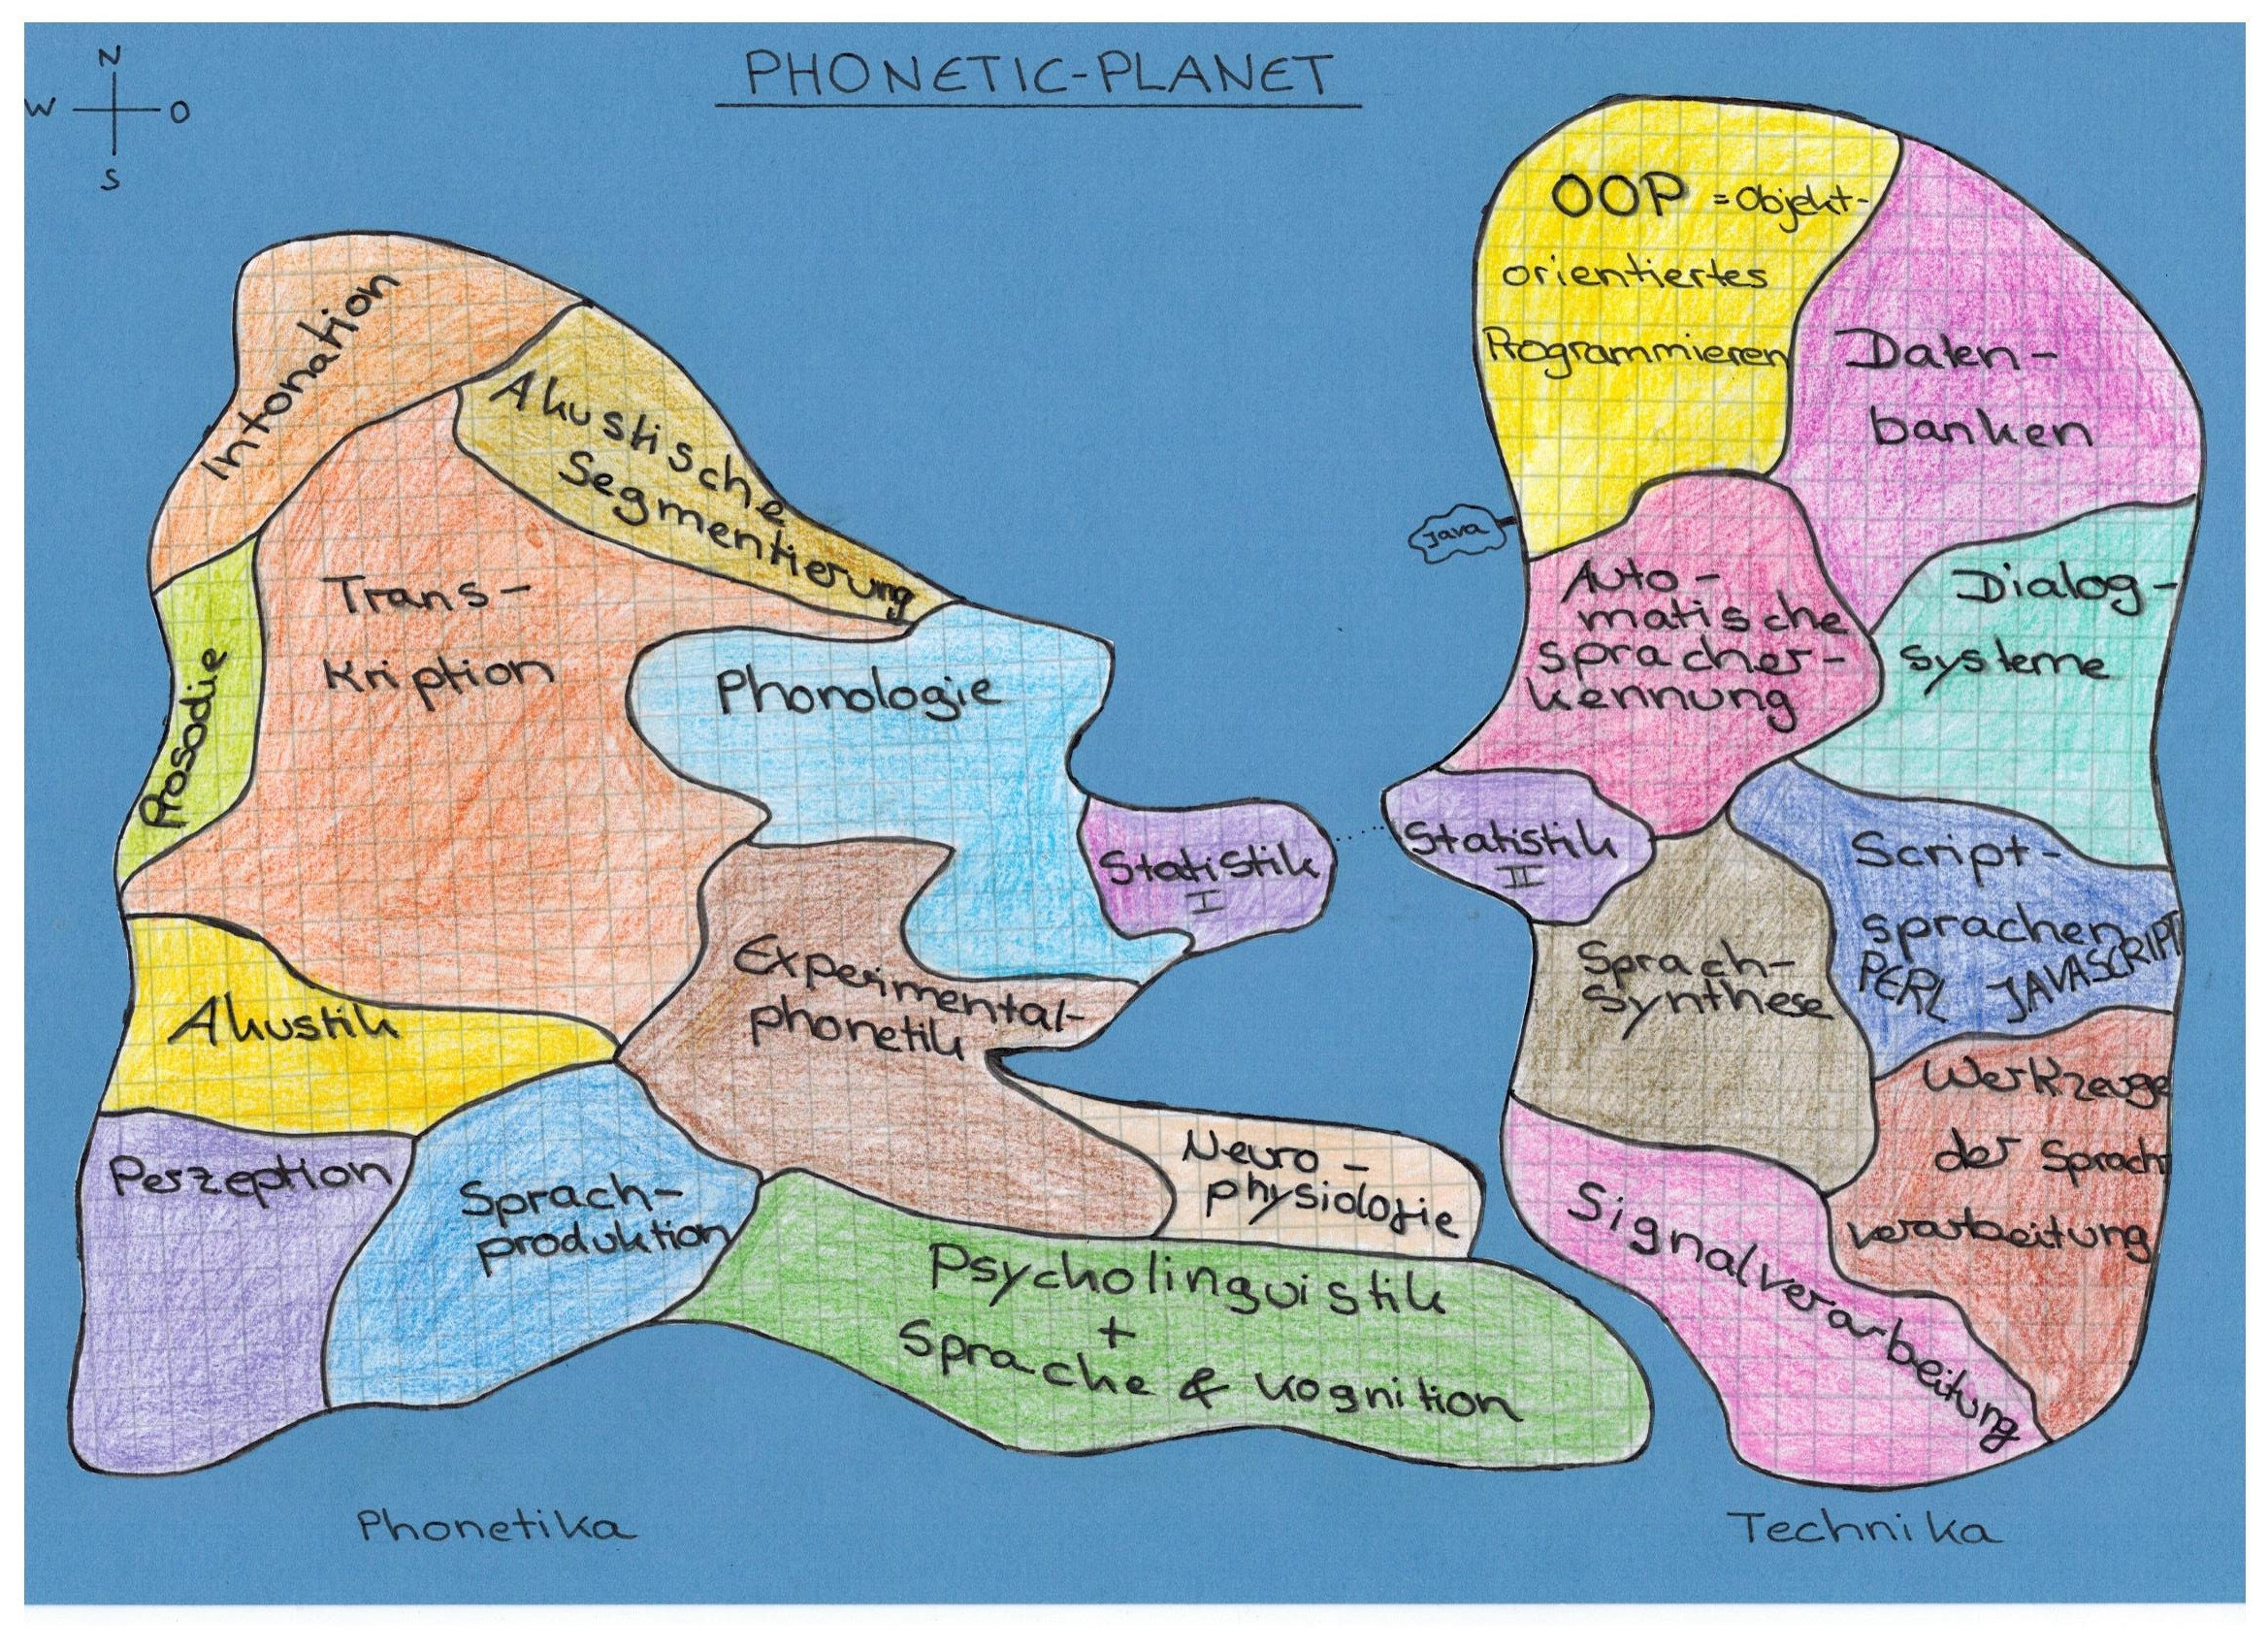
\includegraphics[width=1.0\textwidth] {grafiken/titel/landkarte.jpg} \\
\end{figure} 

% Title
\newcommand{\HRule}{\rule{\linewidth}{0.5mm}}
\HRule \\[0.3cm]
{ \huge \bfseries Logbuch Phonetik und Sprachverarbeitung}\\
{\bfseries P1.3 Deskriptive Phonetik 2018/19}
\\[0.4cm]
\HRule \\[0.5cm]

% Author and supervisor
\begin{minipage}{0.4\textwidth}
%\begin{flushleft} 
\large
%Autoren:\\
Felicitas Kleber, Florian Schiel, Raphael Winkelmann, Christoph Draxler, Anke Werani 

%\end{flushleft}
\end{minipage}
%\fill

% Unterer Teil der Seite
{\large \today}\vspace {1cm}

\begin{minipage}[cb]{0.1\textwidth}

\includegraphics[width=\textwidth]{grafiken/titel/bmbf.jpg}
\end{minipage}
\begin{minipage}[cb]{0.1\textwidth}
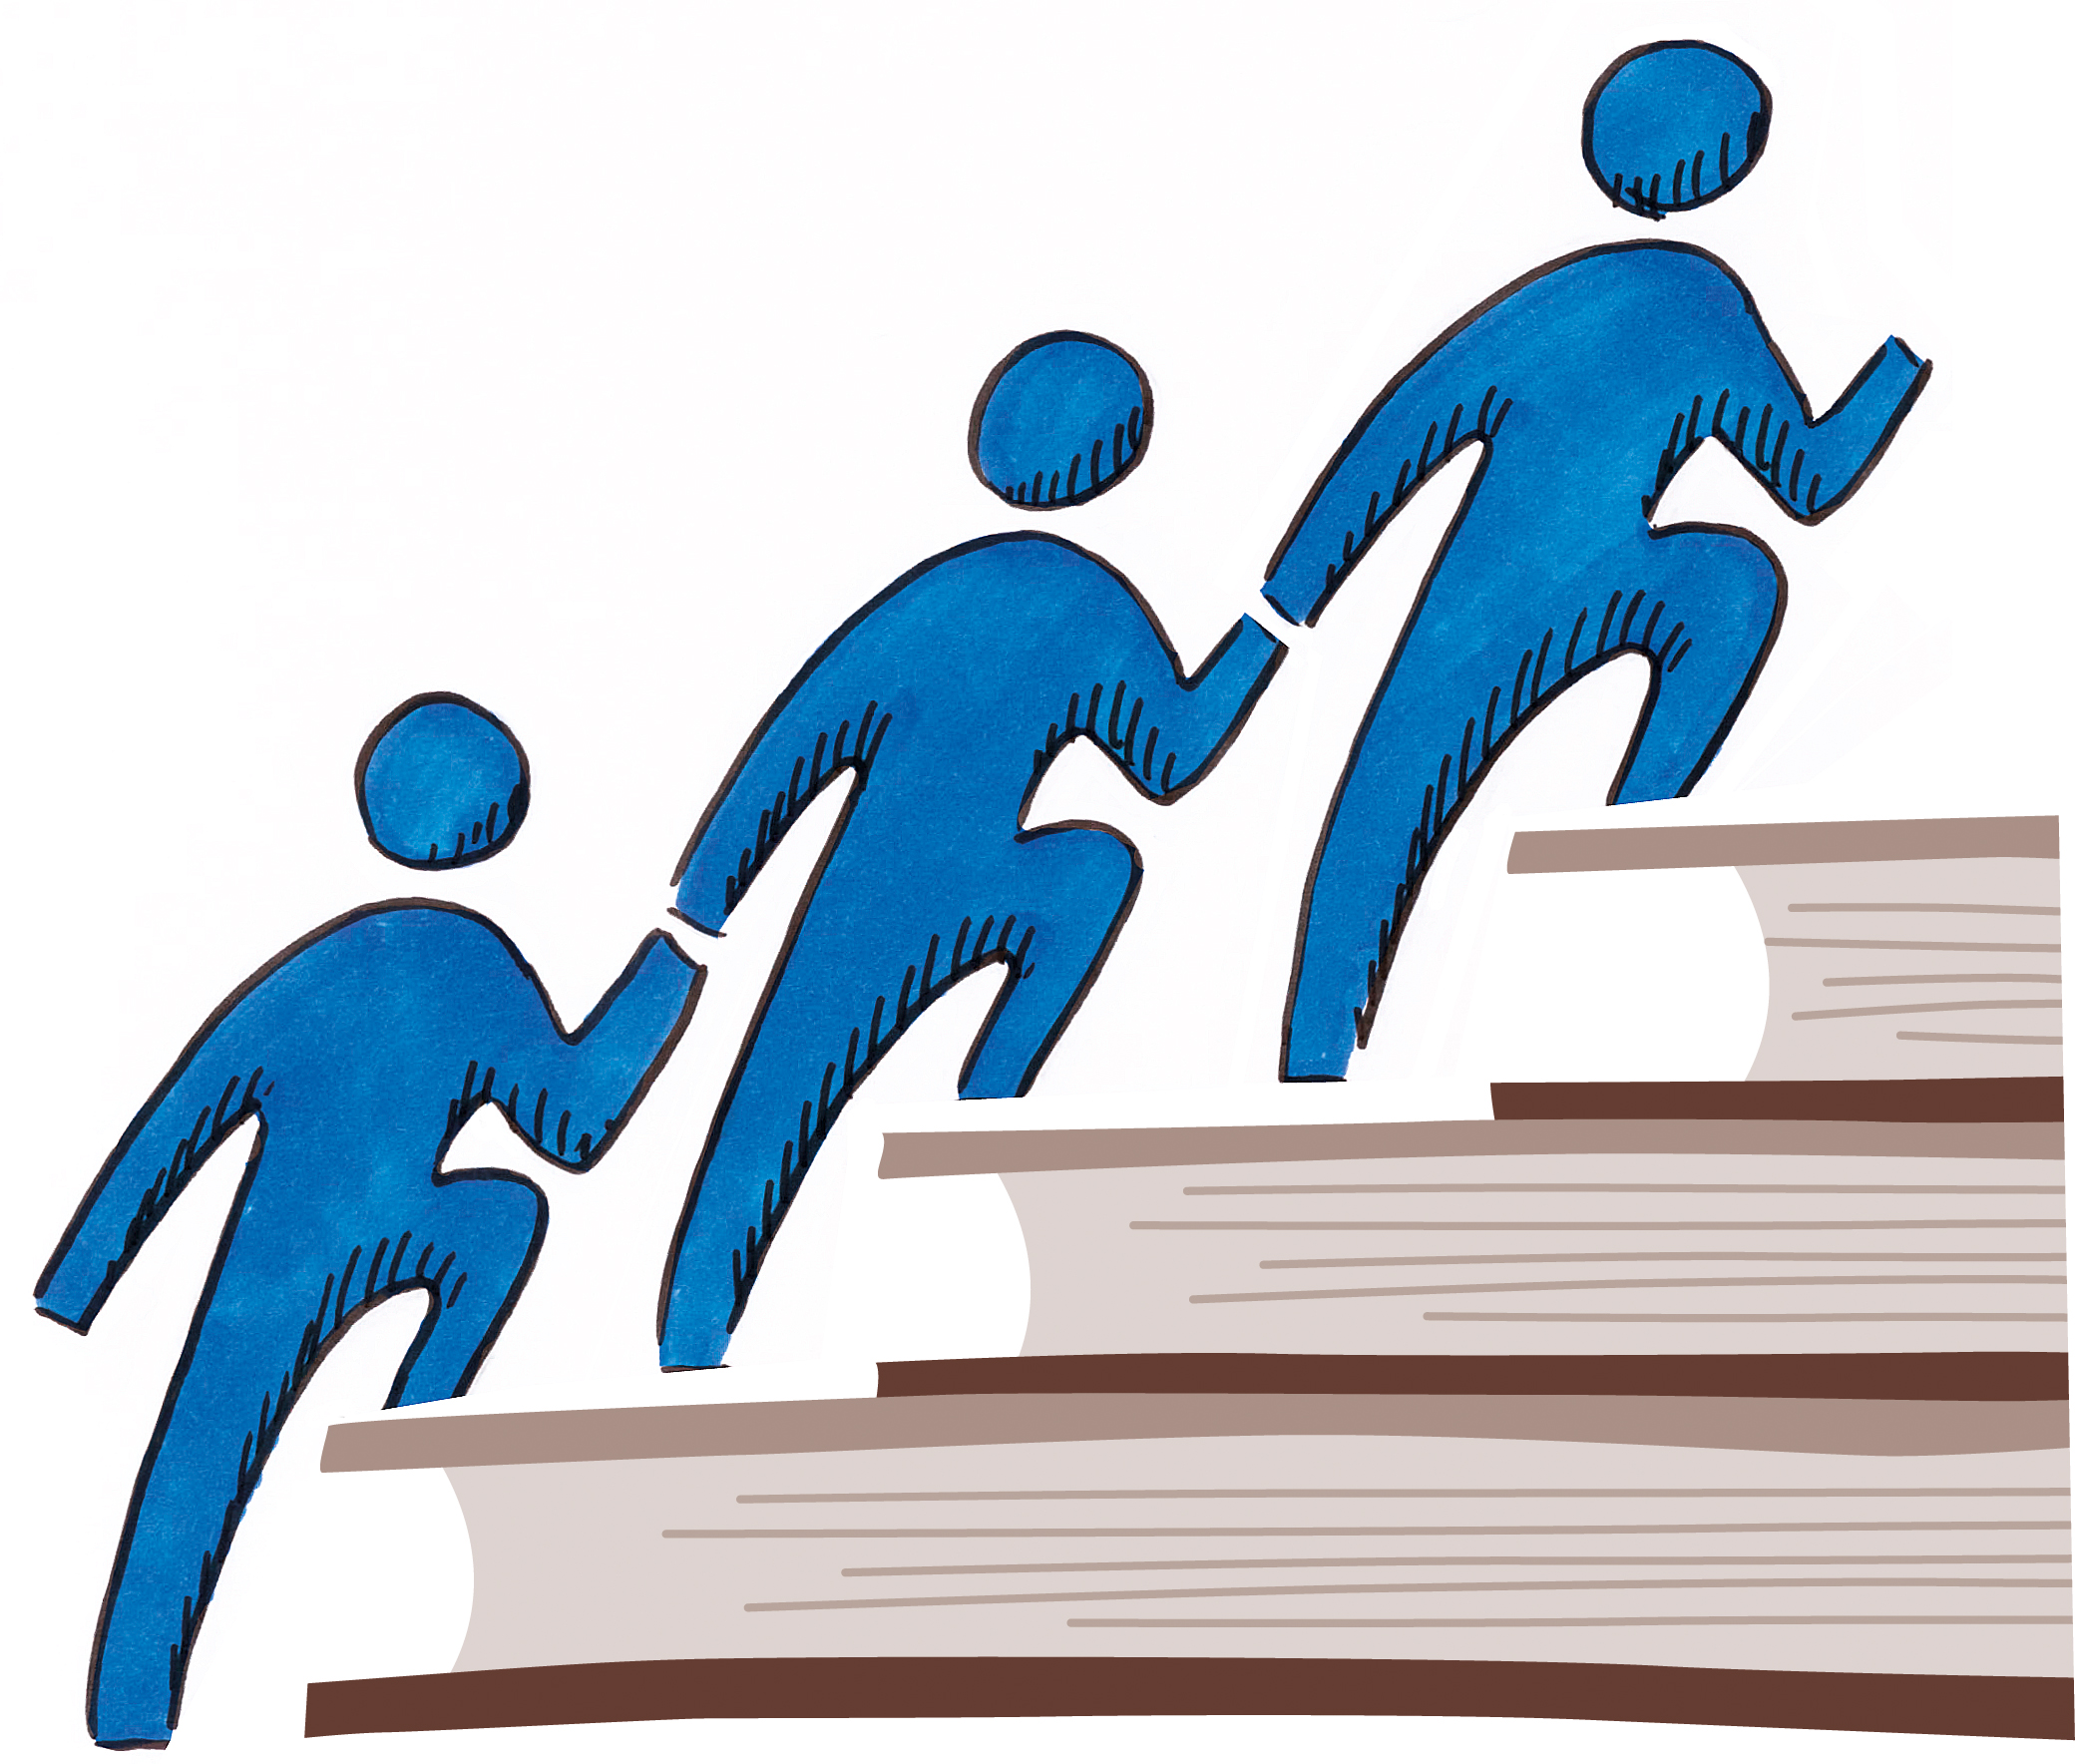
\includegraphics[width=\textwidth]{grafiken/titel/center.jpg}
\end{minipage}
\begin{minipage}[cb]{0.1\textwidth}

\includegraphics[width=\textwidth]{grafiken/titel/lehreatlmu.jpg}
\end{minipage}
\begin{minipage}[cb] {0.1\textwidth}

\includegraphics[width=\textwidth]{grafiken/titel/ips.png}
\end{minipage}


\begin{spacing}{0.2}
\tiny Dieses Teilprojekt wird im Rahmen des Multiplikatoren-Projekts durch den Qualitätspakt Lehre (Lehre@LMU) gefördert. Das Multiplikatoren-Projekt ist an das LMU Center for Leadership and People Management angegliedert. Der Qualitätspakt Lehre wird aus Mitteln des Bundesministeriums für Bildung und Forschung unter dem Förderkennzeichen 01PL12016 gefördert. Die Verantwortung für den Inhalt dieser Veröffentlichung liegt beim Autor \normalsize
\end{spacing}


\newpage

\textbf {Nicht vergessen:\\Erster Stammtisch des Semesters am\\Donnerstag, den 25.10.2018 um 18 Uhr in der Phonetik-Bibliothek!}
%\vspace*{3cm}
%\includegraphics [width=\textwidth]{Abb/Notizzettel.jpg}

\end{center}
\end{titlepage}
\thispagestyle{empty}
\tableofcontents

\chapter{Vorwort}
\textipa {["hE@tslI\c{c}vIl"kOm@n]} am Institut für Phonetik und Sprachverarbeitung (IPS) an der LMU München!
Sie halten hier ein für Sie frisch gedrucktes Logbuch in Händen, und wir hoffen, dass es Sie darin unterstützt, einen Überblick über das Fach \emph{Phonetik und Sprachverarbeitung} zu bekommen.\\
\\
Das Logbuch wurde im Rahmen des Multiplikatoren-Projektes erstellt, einem Teil des Qualitätspakts \emph{Lehre@LMU} der Ludwig-Maximilians-Universität München. Unter dem Motto „Für Lehre begeistern. Kompetent lehren.“ wird mit einem interdisziplinären Projekt versucht die wissenschaftliche Vielfalt im Fach Phonetik und Sprachverarbeitung für Studierende deutlicher zu machen. An dieser Stelle gilt unser herzlicher Dank unseren engagierten studentischen Hilfskräften Katharina Juhl, Daniela Pilz und Korbinian Slavik, die durch rege Diskussion den Aufbau mitgestaltet und schlussendlich die gut lesbare Form ermöglicht (ge\TeX{}t ;-)) haben.\\
\\
Das Logbuch ermöglicht Ihnen zweierlei: zum einen erhalten Sie einen Überblick über das Fach Phonetik und Sprachverarbeitung – zum anderen ermöglicht Ihnen das Logbuch, eine wissenschaftliche Arbeitstechnik kennenzulernen. Das wissenschaftliche Logbuch dient (gleichwohl dem der Seefahrt) zur Positionsbestimmung, d.\,h. Sie bestimmen kontinuierlich Ihre wissenschaftlichen Positionen, dokumentieren damit Ihre wissenschaftliche Entwicklung. Zudem erleichtert es das wissenschaftliche Schreiben, indem Sie üben aufzuschreiben, worüber Sie nachdenken, was Sie mit KommilitonInnen diskutiert haben oder was Sie allgemein für wichtig halten.\\
\\
Da Sie das Modul \textit{P1 Grundlagen} sowohl in die Phonetik als \textit{Disziplin} als auch in das \textit{Fach} Phonetik und Sprachverarbeitung einführen soll, ist der Titel dieser Lehrveranstaltung \emph{Deskriptive Phonetik} etwas weiter zu fassen. Zur Erläuterung hierzu eine kleine Anmerkung: Das IPS wurde 1972 gegründet und bestand zunächst aus den Fächern Phonetik und Sprechwissenschaft (Psycholinguistik). 1995 wurde das Bayerische Archiv für Sprachsignale (BAS) als öffentliche Einrichtung der LMU gegründet und befindet sich seitdem am IPS. Die Mitarbeiter des BAS forschen v.\,a. im sprachtechnologischen Bereich. Historisch gewachsen finden sich damit an unserem Institut die Disziplinen Phonetik, Psycholinguistik und Sprachtechnologie.  Die drei Disziplinen und Teile ihrer Inhalte wurden im Zuge des Bologna-Prozesses 2009 in Module des Faches Phonetik und Sprachverarbeitung umgesetzt. Daher werden Sie in diesem Seminar nicht ausschließlich mit Inhalte der Deskriptiven Phonetik, sondern in kompakter Form mit einem Gesamtüberblick über das Fach konfrontiert. Unser Institut ist in Deutschland das einzige, an dem man Phonetik im Hauptfach studieren kann, und es zählt zu den weltweit innovativsten Forschungslabors. Es bietet Ihnen damit eine einmalig breite und gründliche Ausbildung – nutzen Sie diese Chance!\\

Im Aufbau des Logbuchs lassen sich zwei Teile erkennen:
\begin{itemize}
      \item Der Teil Deskriptive Phonetik ist vor allem durch Übungen gekennzeichnet. Die zentralen Inhalte der Deskriptiven Phonetik hören Sie in der Vorlesung. Da die Vorlesung mit diesem Seminar abgestimmt ist, profitieren Sie am meisten von diesem Seminar, wenn Sie die Inhalte der Vorlesung gehört und vertieft haben.
      
      \item Der Teil, der die Disziplinen Sprachtechnologie und Psycholinguistik repräsentiert, enthält zentrale Inhalte der Kurzvorträge (daher mehr Text) und ebenfalls Übungen, die sie mit den Inhalten vertraut machen sollen.
   \end{itemize}

In allen Kapiteln finden Sie zu Beginn  Cartoons, die helfen sollen, die Inhalte grafisch zu fassen und in Beziehung zu setzen. Wir sind noch auf der Suche nach einer einheitlichen \textit{Topographie}, die alle Inhalte und deren Zusammenhänge grafisch verdeutlicht. Hier sind wir noch im Prozess und freuen uns über Rückmeldungen, wie Sie für sich eine Topographie, eine grafische Verortung des Faches, vornehmen würden. Insofern verstehen Sie dieses Logbuch tatsächlich als Arbeitsbuch. Ihre Anregungen, Kommentare, Korrekturen sind uns gerne willkommen.\\
\\
So, nun sind wir gespannt, ob dieses Logbuch einen Beitrag dazu leisten kann, unserem Ziel näher zu kommen, Ihnen eine Einführung und einen Überblick über das Fach Phonetik und Sprachverarbeitung zu ermöglichen und bereits erste Zusammenhänge zwischen den einzelnen Disziplinen aufzudecken.\\
\\
Einen guten Start für Ihre wissenschaftliche Reise!
\begin {flushright} 
Oktober 2017
\end{flushright}
Christoph Draxler, Felicitas Kleber, Florian Schiel, Anke Werani, Raphael Winkelmann





\chapter{Allgemeine Einführung}

Im weitesten Sinne kann man die Phonetik als die Wissenschaft der gesprochenen Sprache beschreiben. In der ersten Sitzung der Grundlagen-Vorlesung „Phonetik“ wurde eine Reihe differenzierter Definitionen präsentiert, bei denen vor allem die Sprachproduktion (\textit{Artikulation}), Transmission (\textit{Akustik}) und \textit{Perzeption} im Vordergrund stehen. Bei der Erforschung gesprochener Sprache kommen \textit{signalphonetische} und \textit{symbolphonetische} Untersuchungsansätze zur Anwendung. $\rightarrow$ {\tt L1\underline{\ }Einführung.pdf} 

Die \textit{Sprachkette} und das \textit{signalphonetische} Band stellen die oben genannten Bereiche der Phonetik graphisch dar. Des Weiteren können in ihr die Neurophonetik, die sich mit der Sprechplanung und Sprachverarbeitung im Gehirn beschäftigt, sowie die Psycholinguistik, die unter anderem die menschliche Sprachfähigkeit untersucht, verortet werden.  Um den Bereich der Sprachtechnologie in der Sprachkette abzubilden müssen entweder der Sprecher (Sprachsynthese) und/oder der Hörer durch Computer   ausgetauscht werden. Das Prinzip der Sprachkette bleibt bestehen, aber die Komponenten müssen geändert bzw. ergänzt werden und Untersuchungsgegenstände ändern sich teilweise.

Während die Vorlesung vorrangig Artikulation, Akustik und Perzeption und darüber hinaus die Phonologie, d.\thinspace h. die Lehre von den Funktionen von Lauten in einer Sprache,  behandelt, werden in dieser Übung auch die anderen oben genannten Aspekte der Sprachkette beleuchtet und in einen phonetischen Gesamtrahmen eingebettet. Das Kapitel „Deskriptive Phonetik und Phonologie“ greift die Themen der Vorlesung auf und bietet Begleitübungen und Diskussionsgrundlagen. Eigene Sprachaufnahmen und ein erstes Kennenlernen phonetischer Werkzeuge dienen dem Einstieg in das wissenschaftliche Arbeiten.


\begin{figure}[htbp]
\begin{center}
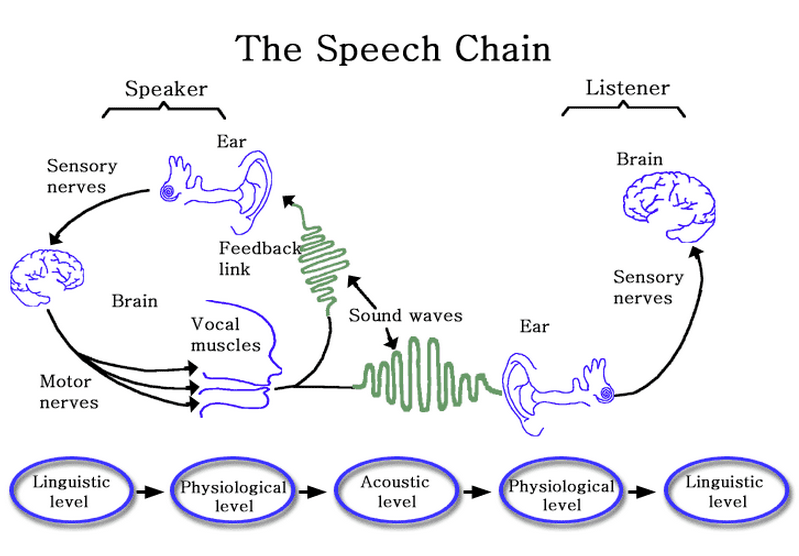
\includegraphics[width=\textwidth]{grafiken/allgemeine-einfuehrung/speech-chain}
\caption{nach Denes, P. B.; Pinson, E. N. (2012). The Speech Chain. The Physics And Biology Of Spoken Language.}
\label{fig1}
\end{center}
\end{figure}

\section{Stichworte zur ersten Stunde der Vorlesung} 

ABC-Prosodie,  Symbol- vs. Signalphonetik, Signalphonetisches Band, Sprachkette, Sprachlaut... $\rightarrow$ {\tt L1\underline{\ }Einführung.pdf} 


\section{Literatur}

Borden, G. J.; Harris, K. S., Raphael, L. J. (2011). Speech science primer. Physiology, acoustics, and perception of speech. 6. Aufl. Baltimore: Lippincott Williams \& Wilkins. \newline\\
Bußmann, H. (2008). Lexikon der Sprachwissenschaft. 4. Aufl. Stuttgart: Kröner. \newline\\
Clark, J. \& Yallop, C. (2007). An introduction to phonetics and phonology. Malden u.\,a.:  Basil Blackwell.\newline\\
Gussenhoven, C. \& Jacobs, H. (2011). Understanding Phonology. London  u.\,a.: Hodder.\newline\\
Hall, T. A. (2011). Phonologie: Eine Einführung. 2. Aufl. Berlin: Walter de Gruyter. \newline\\
International Phonetic Association (Hrsg.)(1999). \textit{Handbook of the International Phonetic Association}. Cambridge: Cambridge University Press. \newline\\
Kohler, K. J.(1995). Einführung in die Phonetik des Deutschen. Berlin: Erich Schmidt. \newline\\
Ladefoged, P.; Johnson, K.  (2014). A course in phonetics. 7.\,Aufl. Stamford u.\,a.: Cengage Learning. \newline\\
Ladefoged, P. \& Ferrari, S. (2012). Vowels and consonants. An introduction to the sounds of language. 3.\,Aufl. Chichester: Wiley-Blackwell. \newline\\
Pompino-Marschall, B. (2009). Einführung in die Phonetik. 3. Aufl. Berlin/New York: de Gruyter.  \newline\\
Reetz, H. (2003). Artikulatorische und akustische Phonetik. 2.\,Aufl. Trier: Wissenschaftlicher Verlag.  \newline\\
Spencer, A. (1996). Phonology. Oxford: Blackwell.\newline\\
Tillmann, H. G. \& Mansell, P. (1980). Phonetik: Lautsprachliche Zeichen, Sprachsignale und lautsprachlicher Kommunikationsprozeß. Stuttgart: Klett-Cotta. \newline\\

\section{Interaktives Glossar}

Im Laufe des Semesters werden Ihnen einige Begriffe begegnen, über die Sie mehr wissen wollen oder mit denen Sie noch nicht soviel anfangen können. Hier haben Sie die Möglichkeit sich diese Wörter zu notieren und selbstständig, bzw. mit unserer Hilfe, Erklärungen zu finden. Glossare, Indexe oder Register finden sich in vielen der oben genannten Bücher; z.\,B. in Pompino-Marschall\,(2009), Reetz\,(2003), Draxler\,(2008) oder in Ladefoged \& Ferrari\,(2012). Bei Fragen stehen wir ihnen gerne zur Verfügung.  





\chapter{Sprechen}

\section{Stichworte zur Vorlesung \em{Artikulatorische Phonetik}} 

Sprechen als aerodynamischer Prozess, Kehlkopf/Larynx, Stimmlippen(schwingung), Phonation, Vokaltrakt... $\rightarrow$ {\tt L2\underline{\ }Artikulation.pdf}

\begin{figure}[htbp]
\begin{center}
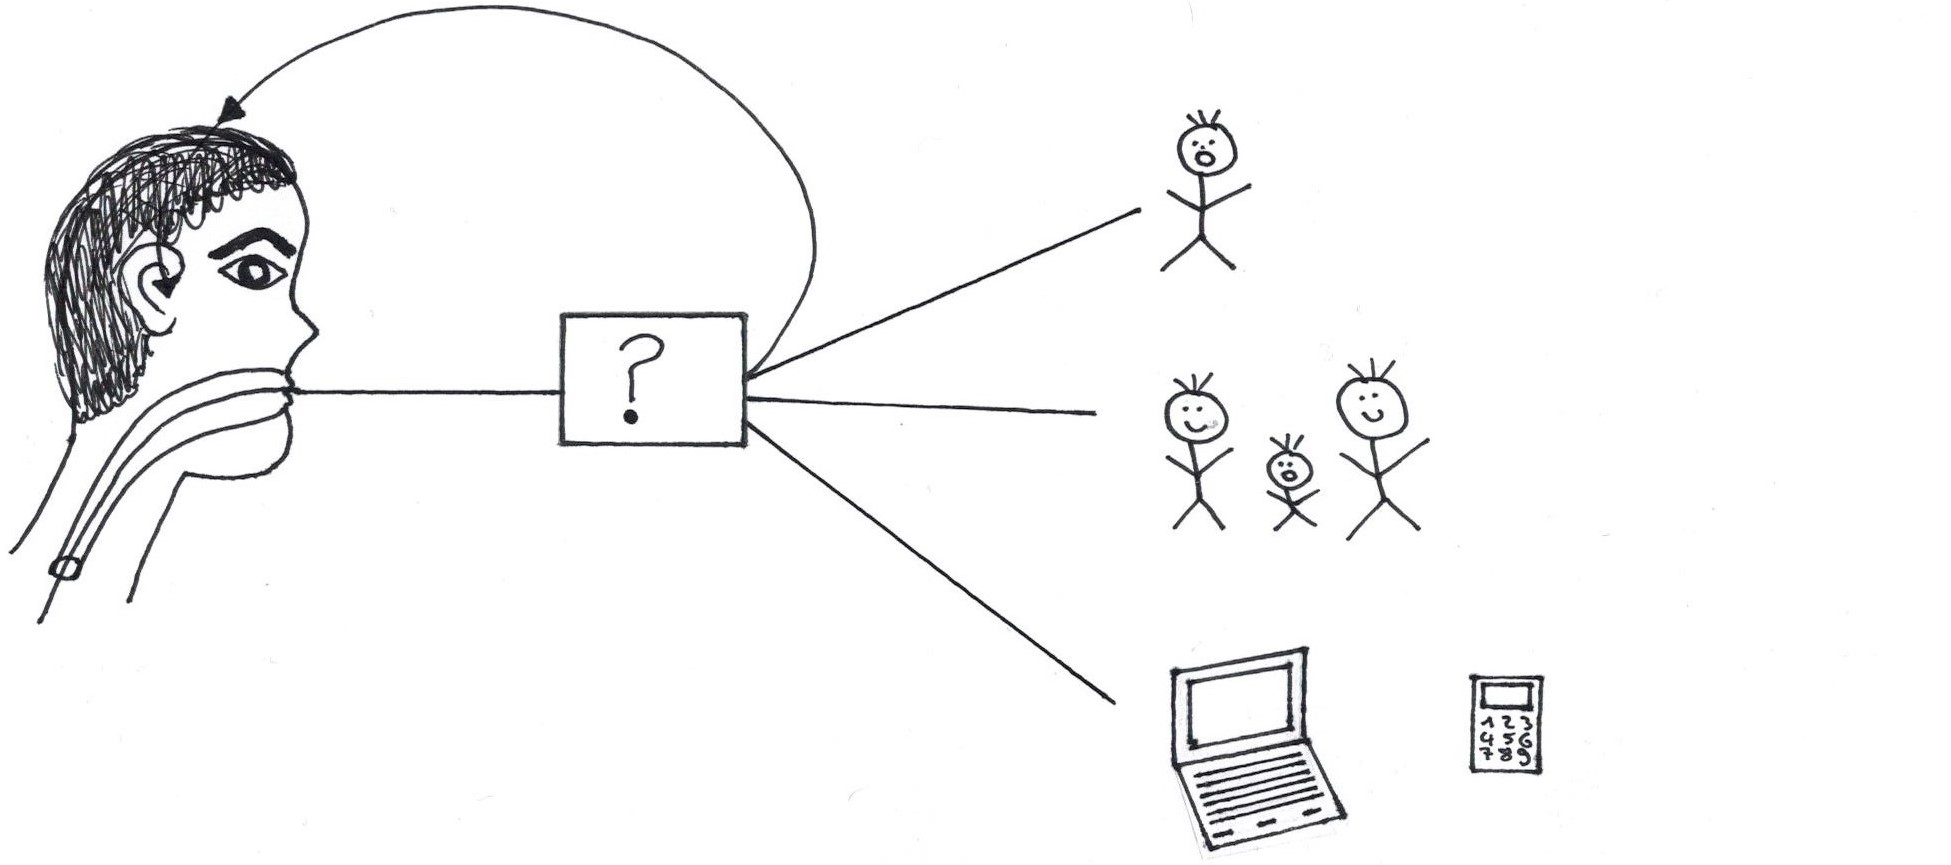
\includegraphics[width=\textwidth]{grafiken/sprechen/sprechen}
\label{t1}
\end{center}
\end{figure}



\section{Aufgabenstellungen}

1.	Wie viele Sprachlaute gibt es ihrer Meinung nach im Deutschen? Listen Sie sie auf und notieren Sie Beispielwörter, in denen diese vorkommen.
\vspace*{7cm}


2. Beschriften Sie bitte die nachfolgende Abbildung.
\begin{figure}[htbp]
\begin{center}
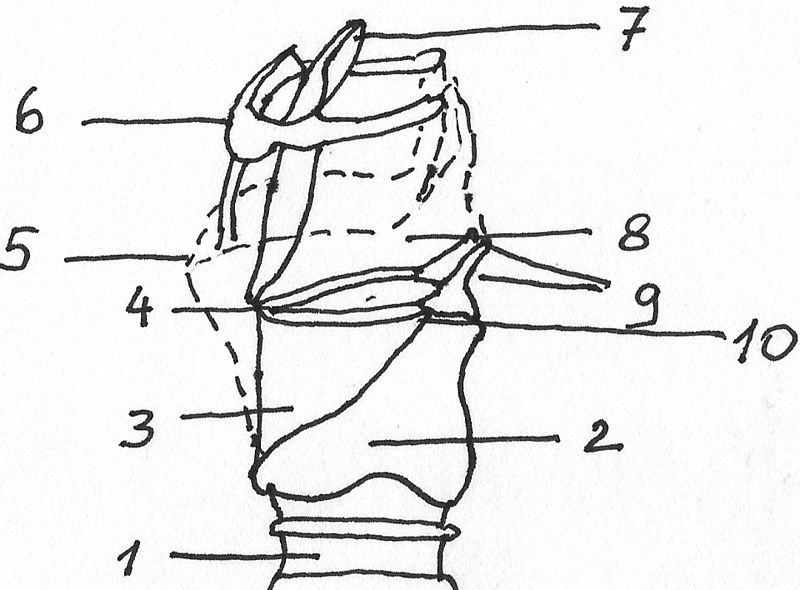
\includegraphics[scale=3]{grafiken/sprechen/kehlkopf}
\caption{Kehlkopf}
\label{fig2}
\end{center}
\end{figure}

\newpage
3.	Benennen Sie die nummerierten Bereiche des nachfolgend abgebildeten Vokaltraktes:
\begin{figure}[htbp]
\begin{center}
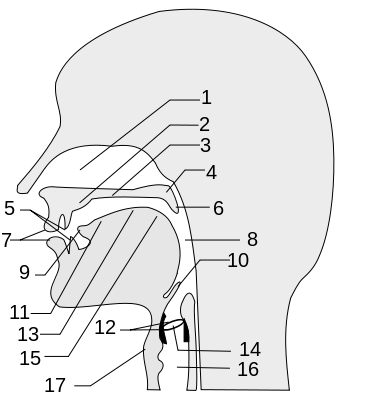
\includegraphics[scale=0.6]{grafiken/sprechen/kopf}
\caption{©  Tavin /Wikimedia Commons / CC-BY-3.0}
\label{fig3}
\end{center}
\end{figure}

4.	Welche Sprechorgane neben den Stimmlippen haben aerodynamische Funktionen?
\begin{figure}[htbp]
\begin{center}
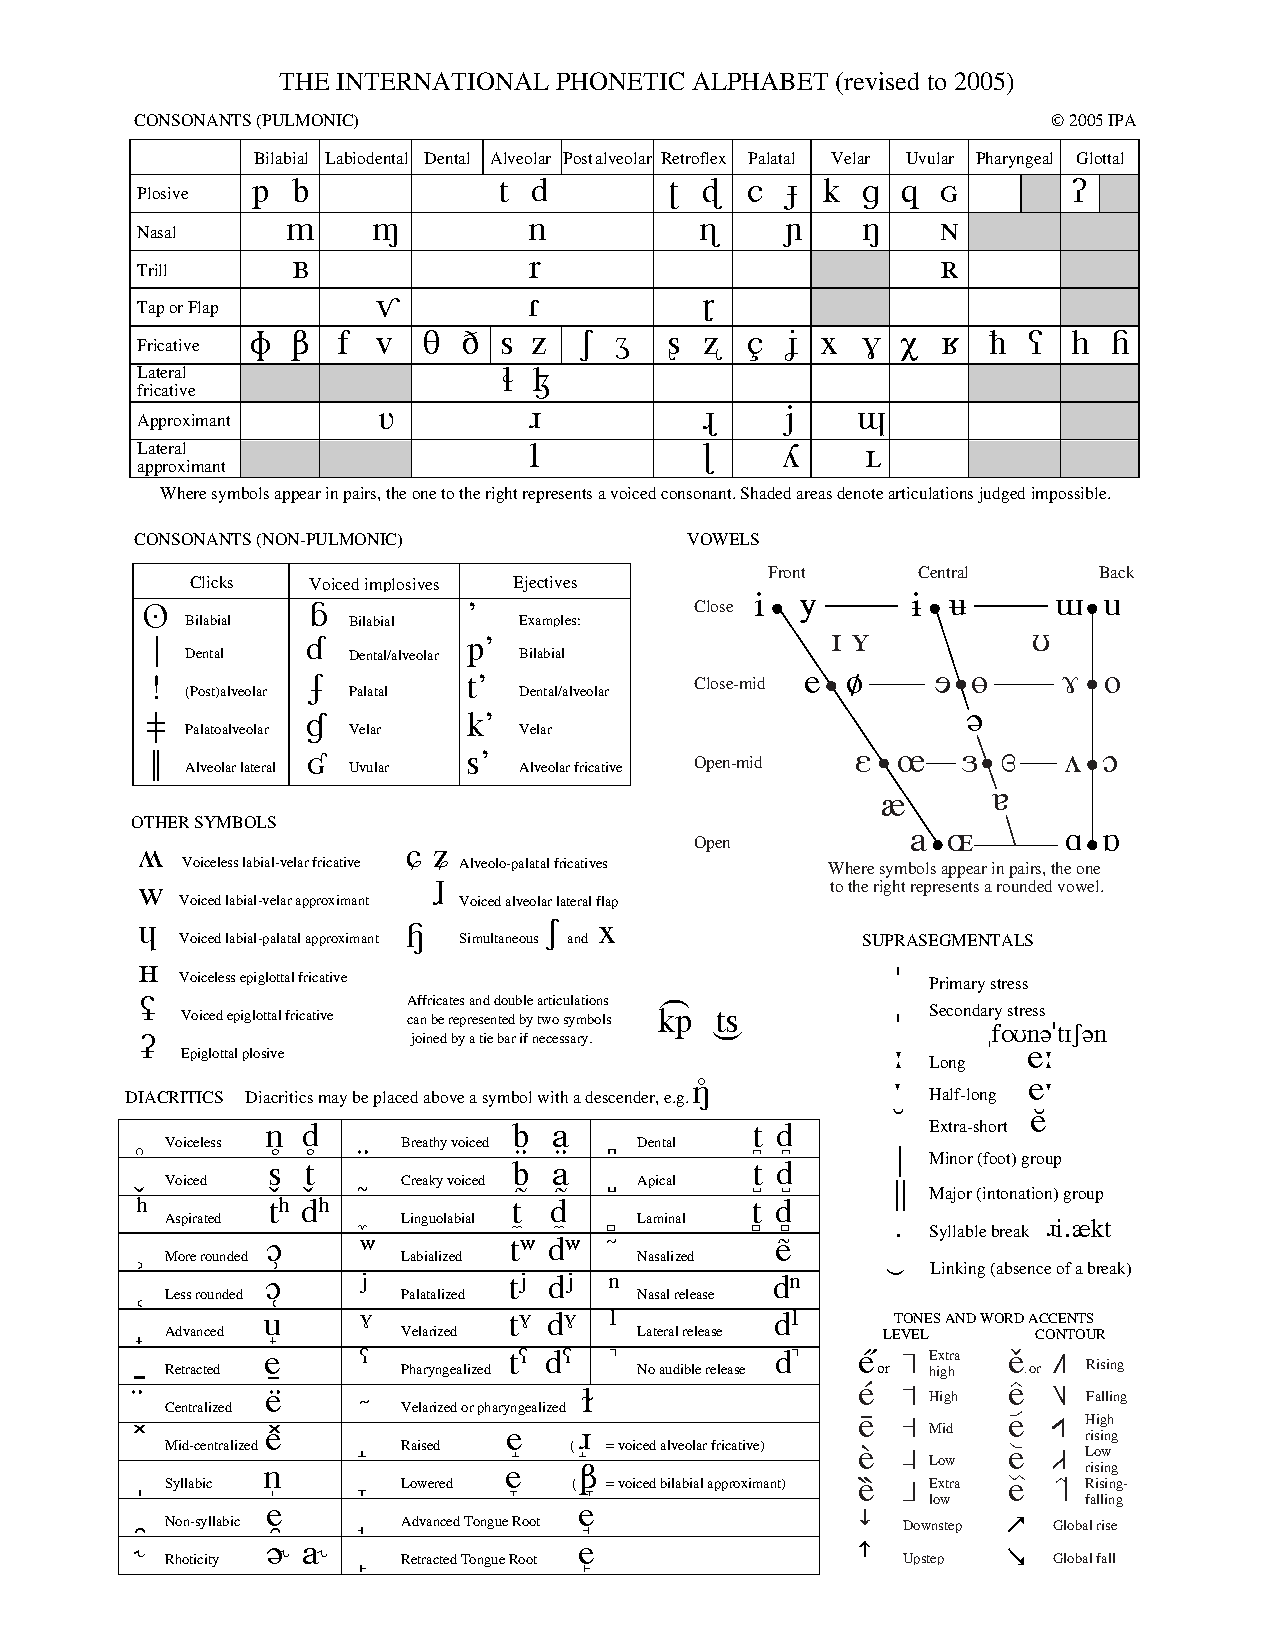
\includegraphics[width=\textwidth]{grafiken/sprechen/ipa}
\caption{IPA-Tabelle}
\label{fig4}
\end{center}
\end{figure}

\newpage
\begin{figure}[htbp]
\begin{center}
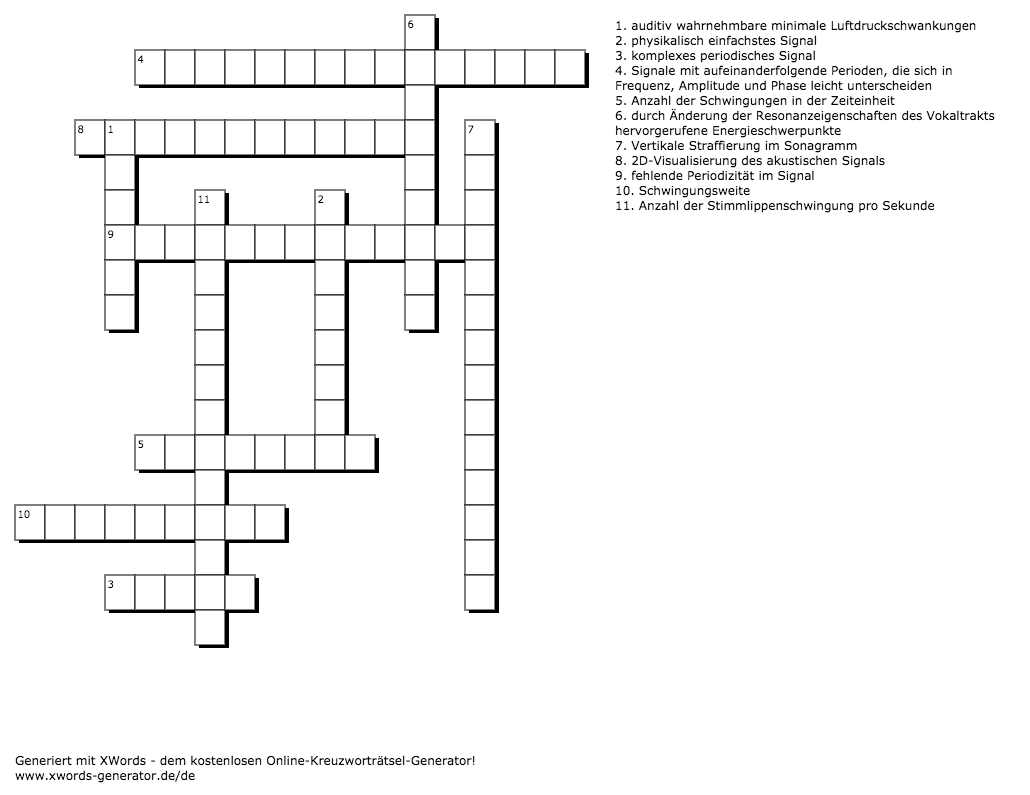
\includegraphics[width=1.2\textwidth]{grafiken/sprechen/kreuzwortraetsel}
\caption{Kreuzworträtsel}
\label{fig5}
\end{center}
\end{figure}

\vspace*{\fill} 






\chapter{Fragestellungen und Recherche}


\section{Aufgabenstellungen}

1.	Die Gründe für eine Studienfachwahl und die Erwartungen an das letztendlich gewählte Fach sind vielfältig.  Welche Fragen stellen sich Ihnen, wenn Sie an Phonetik denken? Worauf hätten Sie gerne eine Antwort, die man ihrer Meinung nach nur mit phonetischem Fachwissen geben kann? Diskutieren Sie in der Gruppe Ihre Fragen an die Phonetik und wählen Sie gemeinsam eine aus, die Sie besonders interessant finden.\\
\newpage
a.	Formulieren Sie die Fragestellung auf eine präzise Weise.

\vspace*{5cm}


b.	Suchen Sie mithilfe Ihrer elektronischen Geräte im Online Katalog der Universitätsbibliothek nach Büchern, die Ihnen bei der Klärung der Frage helfen können. Notieren Sie Stichworte und Suchergebnisse.
\vspace*{5cm}



\chapter{Sprachaufnahme: Sprechen erfassen und sichtbar machen} 

Gesprochene Sprache ist flüchtig. Um die Transmission von Sprachschall zwischen Schallquelle (z.\thinspace B. Sprecher*in) und Schallsenke (z.\thinspace B. Hörer*in) genau untersuchen zu können (also nicht mittels synchroner Transkription), muss der Sprachschall durch eine Sprachaufnahme festgehalten werden (vgl. auch Kapitel Sprachdatenbanken). 

\section{Stichworte zur Vorlesung \em{Sprachakustik}}

Schall, Schwingung, akustische Signaltypen, (Grund-)Frequenz, Formanten, Oszillogramm, Spektrum, Spektrogramm, Quelle-Filter... $\rightarrow$ {\tt L3\underline{\ }Akustik.pdf}
\begin{figure}[htbp]
\begin{center}
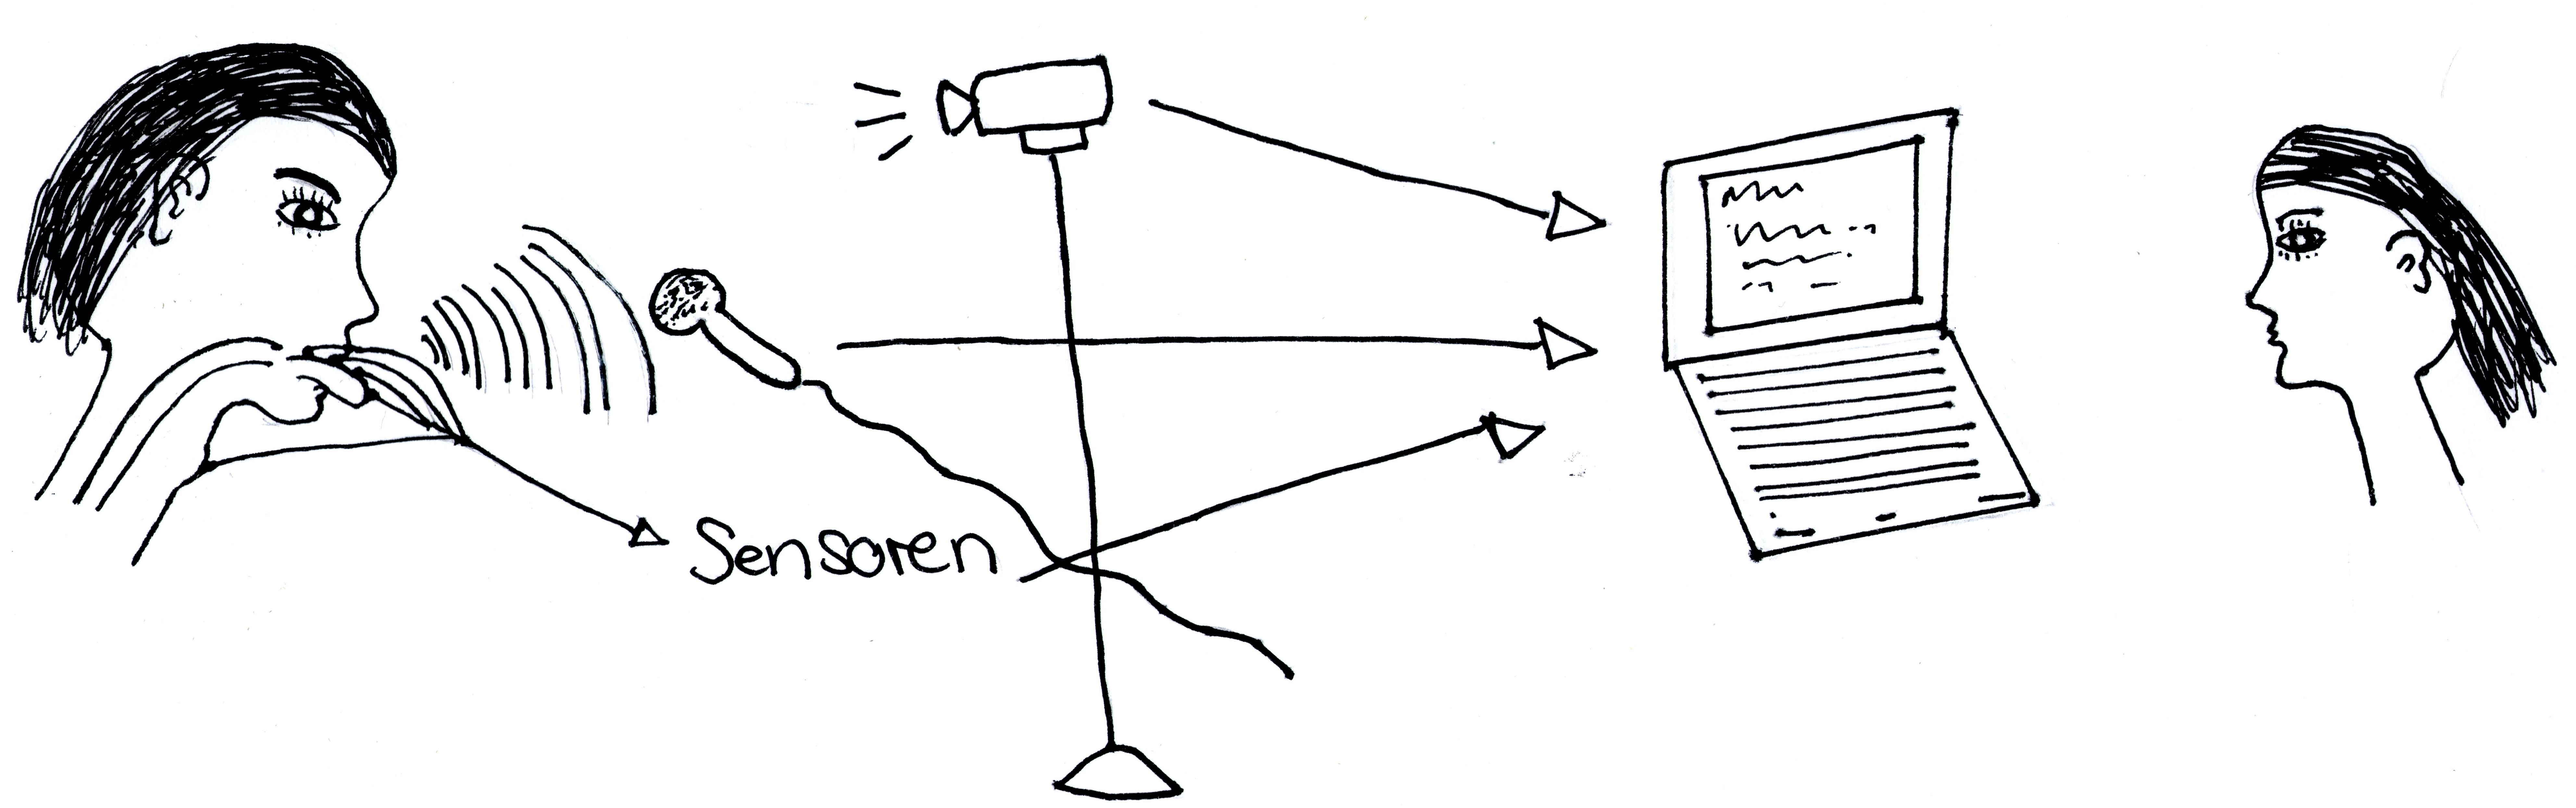
\includegraphics[width=\textwidth]{grafiken/sprachaufnahme/sprechen-erfassen}
\label{t2}
\end{center}
\end{figure}

\section{Aufnahmeübung}


Die Sprachaufnahme erfolgt in Kleingruppen an den mitgebrachten Laptops. Jede Gruppe erhält einen schriftlichen Arbeitsauftrag und ggf. ein Mikrofon oder Aufnahmegerät. Führen Sie die Aufnahme wie angegeben durch und sichern Sie die Audiodateien. In der nächsten Stunde werden wir auf die Dateien zurückgreifen.
\vspace*{7cm} 

Tipp: \newline \\ 
\begin {minipage} {0.1\textwidth}
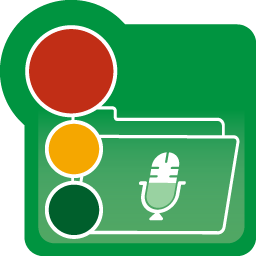
\includegraphics[width=\textwidth]{grafiken/sprachaufnahme/speechrecorder.png}
\end{minipage}
\hspace{1cm}
\begin{minipage} {0.6\textwidth}
Den SpeechRecorder können Sie kostenlos unter {\tt www.bas.uni-muenchen.de/Bas/software/speechrecorder/} (Stand: \today) herunterladen.
\end {minipage}

\begin {minipage} {0.1\textwidth}

\includegraphics[width=\textwidth]{grafiken/sprachaufnahme/praat.png}
\end{minipage}
\hspace {1cm}
\begin{minipage} {0.7\textwidth}
Praat können Sie kostenlos unter {\tt www.fon.hum.uva.nl/praat/} (Stand: \today) herunterladen. 
\end {minipage}



\chapter{Annotationstypen}

Sprachaufnahmen können sowohl symbol- als auch signalphonetisch analysiert werden. In der Regel, insbesondere im Vorfeld einer Datenbankerstellung, werden die Sprachaufnahmen anschließend segmentiert, also in kleinere sprachliche Einheiten (z.\thinspace B. Wörter, Silben, Laute etc.) zerlegt und etikettiert, d.\thinspace h. mit Symbolen versehen. Für die Etikettierung stehen verschiedene Annotationstypen zur Verfügung. Die Segmentierung und Etikettierung basiert häufig auf unserer auditiven Perzeption.

\section{Stichworte zur Vorlesung \em{Sprachperzeption}}

Gehörknöchelchen, Hebelwirkung, Cochlea, Haarzellen, Wanderwelle, Psychoakustik, Kategoriale Wahrnehmung\dots $\rightarrow$ {\tt L4\underline{\ }Perzeption.pdf}

\begin{figure}[htbp]
\begin{center}
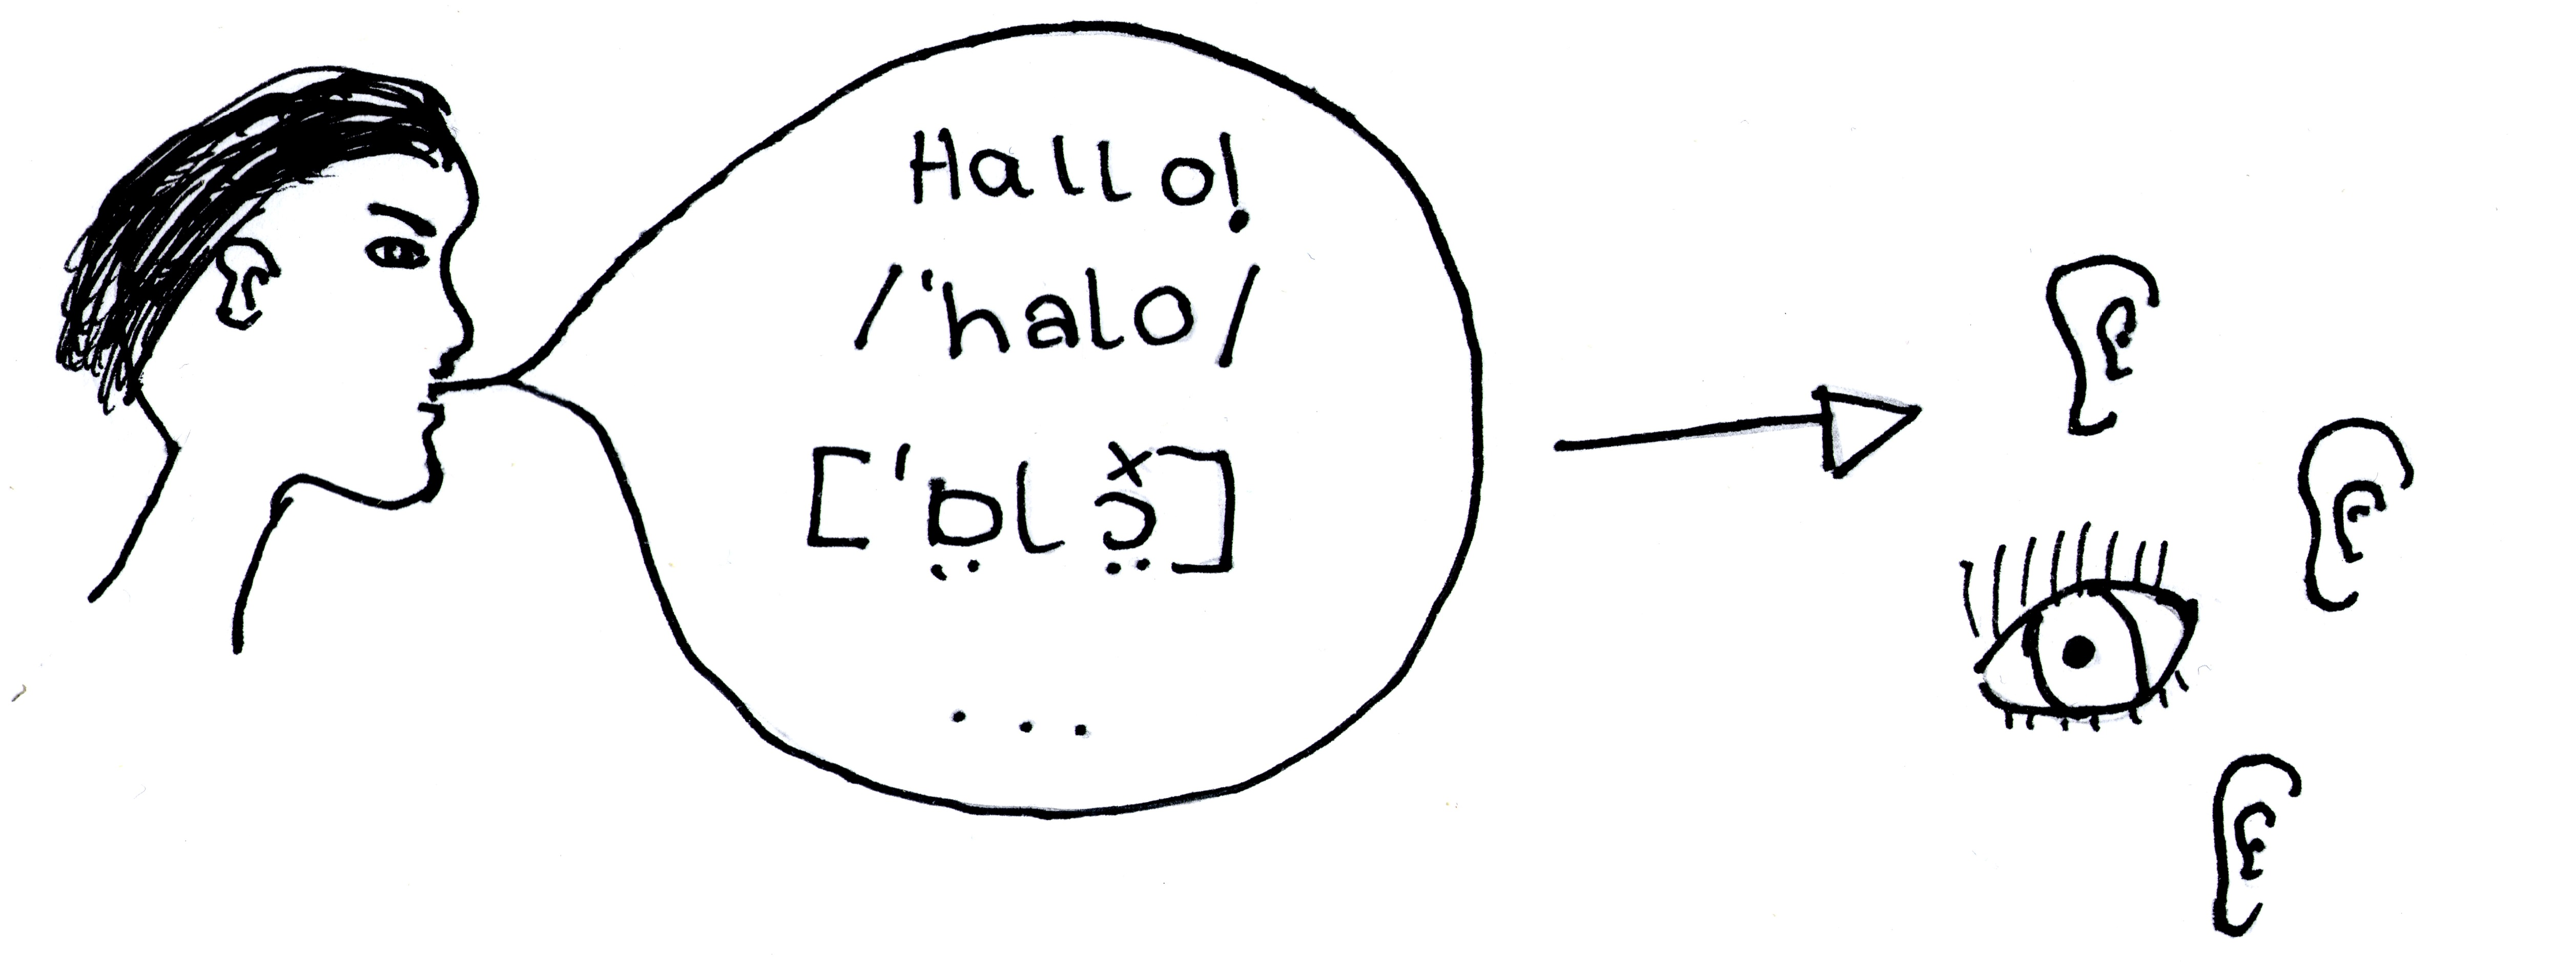
\includegraphics[width=\textwidth]{grafiken/annotationstypen/annotationstypen}
\label{t3}
\end{center}
\end{figure}
\section{Aufgabenstellung}
 
1.	Öffnen Sie den ersten Satz aus ihrem Dialog in Praat ($\rightarrow$ {\tt praat.pdf}) und erzeugen Sie ein TextGrid-File mit zwei \emph{interval tiers} (1 = Wort, 2 = Segment). Öffnen Sie beide Dateien und segmentieren Sie auf der oberen Ebene (\emph{Wort-tier}) die Wörter und auf der unteren Ebene (\emph{Segment-tier}) die Sprachlaute. Für die Etikettierung der Wörter und Laute verwenden Sie bitte die Buchstaben des Deutschen. Notieren Sie ihre Beobachtung zu folgenden Fragen.\\
\newline

a.	Wie genau lassen sich Grenzen zwischen zwei Wörtern bzw. zwischen zwei Sprachlauten setzen? Notieren Sie einfache und schwierige Beispiele. \vspace{5cm}\\
b.	Wie stark hilft Ihnen ihre Sprachperzeption beim Segmentieren? \vspace{5cm}\\
\newpage
c.	Ist die Etikettierung der Sprachlaute immer eindeutig? \vspace{5cm}\\
d.	Wie gut eignen sich die Buchstaben für die Etikettierung? \vspace{5cm}\\
e.	Welche anderen akustischen Eigenschaften in der Sprachaufnahme könnte man etikettieren? \vspace*{5cm}\\
\newpage
\section{Notizen zu anderen Annotationstypen} 






\chapter{Beschreibung von Sprachlauten in der Literatur}

Mithilfe von segmentierten und etikettierten Sprachaufnahmen ist es möglich die akustische Ausprägung von Konsonanten und Vokalen genau zu beschreiben und akustische Reize (\emph{acoustic cues}) herauszufiltern, die für die Sprachperzeption relevant sind. Die Beschreibung von Sprachlauten basiert aber in erster Linie auf artikulatorischen und perzeptiven Aspekten. Zum Glück gibt es bereits sehr gute Beschreibungen der Sprachlaute, die in den Sprachen der Welt vorkommen, sodass Sie für diese Übung nicht auf eigene Sprachaufnahmen zurück greifen müssen, sondern sich mithilfe von Fachliteratur ein Bild machen können.

\section{Stichworte zur Vorlesung \em{Konsonanten und Vokale}}
Artikulationsart und -ort, Stimmhaftigkeit, Zungenhöhe und –position, Lippenrundung, Kardinalvokale\dots $\rightarrow$ {\tt L5\underline{\ }Konsonanten{\&}Vokale.pdf}

\section{Aufgabenstellung}
Lesen Sie den Ihrer Gruppe ausgeteilten Text durch und diskutieren Sie im Anschluss in der Gruppe die wichtigsten Informationen. Gehen Sie dabei auch auf die Beschreibungsebenen ein (artikulatorisch, akustisch oder perzeptiv). Im Anschluss werden die Textzusammenfassungen den anderen Gruppen in einer Kurzpräsentation vorgestellt.
\newline
\section{Notizen}
\vspace*{10cm}






\chapter{Stimmhaftigkeit}

\section{Stichworte zur Vorlesung \em{Aerodynamische Prozesse und Phonation}}

ingressiv, egressiv, Ejektiv, Implosiv, Klicklaut, Bernoulli-Prinzip, Voice onset time (VOT), supra- und subglottaler Luftdruck\dots $\rightarrow$ {\tt L6\underline{\ }Phonation.pdf}

\begin{figure}[htbp]
\begin{center}
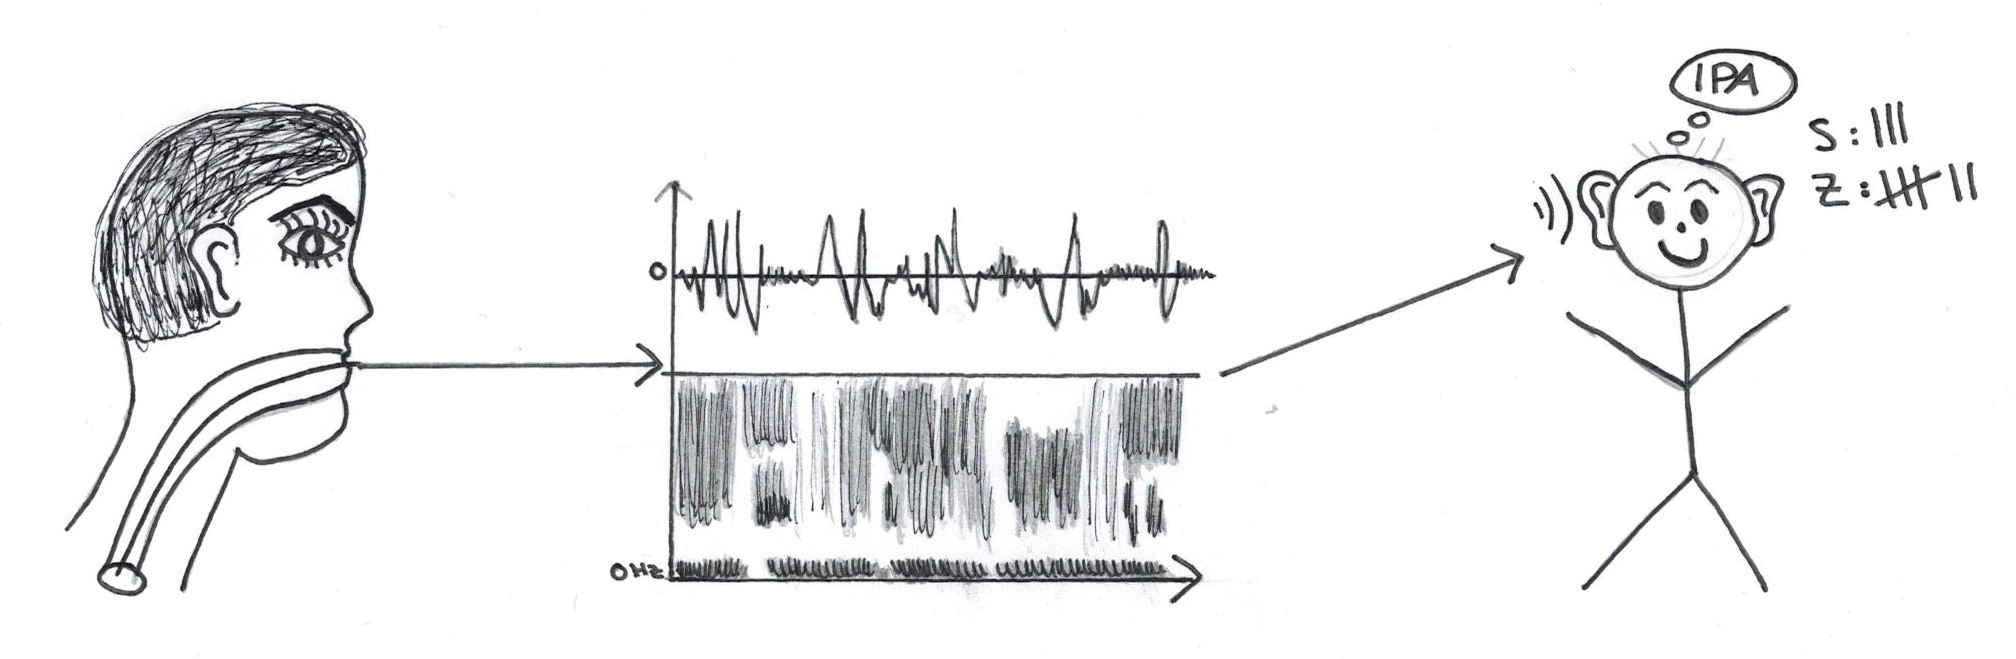
\includegraphics[width=\textwidth]{grafiken/stimmhaftigkeit/stimmhaftigkeit}
\label{t4}
\end{center}
\end{figure}


\newpage
\section{Aufgabenstellungen}

1.	Suchen Sie in Ihren Aufnahmen nach Segmenten, die sie mit einem Symbol etikettiert haben, das Stimmhaftigkeit signalisiert (z.\,B. b, a, n). In welchen Fällen handelt es sich um phonetisch stimmhafte Laute, in welchen nicht?
\vspace{4cm}

2.	Gibt es eine Systematik zwischen stimmhaften Etiketten und fehlender phonetischer Stimmhaftigkeit?
\vspace{4cm}










\chapter{Dialog}
Gesprochene Sprache tritt besonders häufig in Form von \textit{Spontansprache} (z.\,B. im Gegensatz zu Lesesprache) auf, die zudem meistens Teil eines Dialogs ist. Sprachlaute, die in \textit{fließender Rede} in Kombination mit anderen Lauten geäußert werden, weichen in ihrer Form in der Regel von isoliert produzierten Sprachlauten ab (vgl. auch das Kapitel Spontansprachliche Vorgänge), die wiederum der phonetischen Beschreibung zugrunde liegen. Dialoge sind in vielerlei Hinsicht dafür geeignet, spontansprachliche und \textit{suprasegmentale} Eigenschaften in der sprachlichen Kommunikation zu untersuchen, z.\,B. prosodische Mittel zum Halten oder Beenden von \textit{Turns}. Auch in der Sprachtechnologie ($\rightarrow$ Spracherkennung und –synthese) werden zunehmend dialogbasierte Daten berücksichtigt. Viele Kommunikationsmodelle basieren ebenfalls auf dialogisierter Sprache ($\rightarrow$ Psycholinguistik).

\section{Stichworte zur Vorlesung \em{Prosodie und Intonation}}
Grundfrequenz, Tonhöhe, Wortbetonung, Satzakzentuierung, Phrasierung, Deklination, akzent- vs. silbenzählende Sprachen, Paralinguistik... $\rightarrow$ {\tt L7\underline{\ }Prosodie{\&}Intonation.pdf}

\begin{figure}[htbp]
\begin{center}
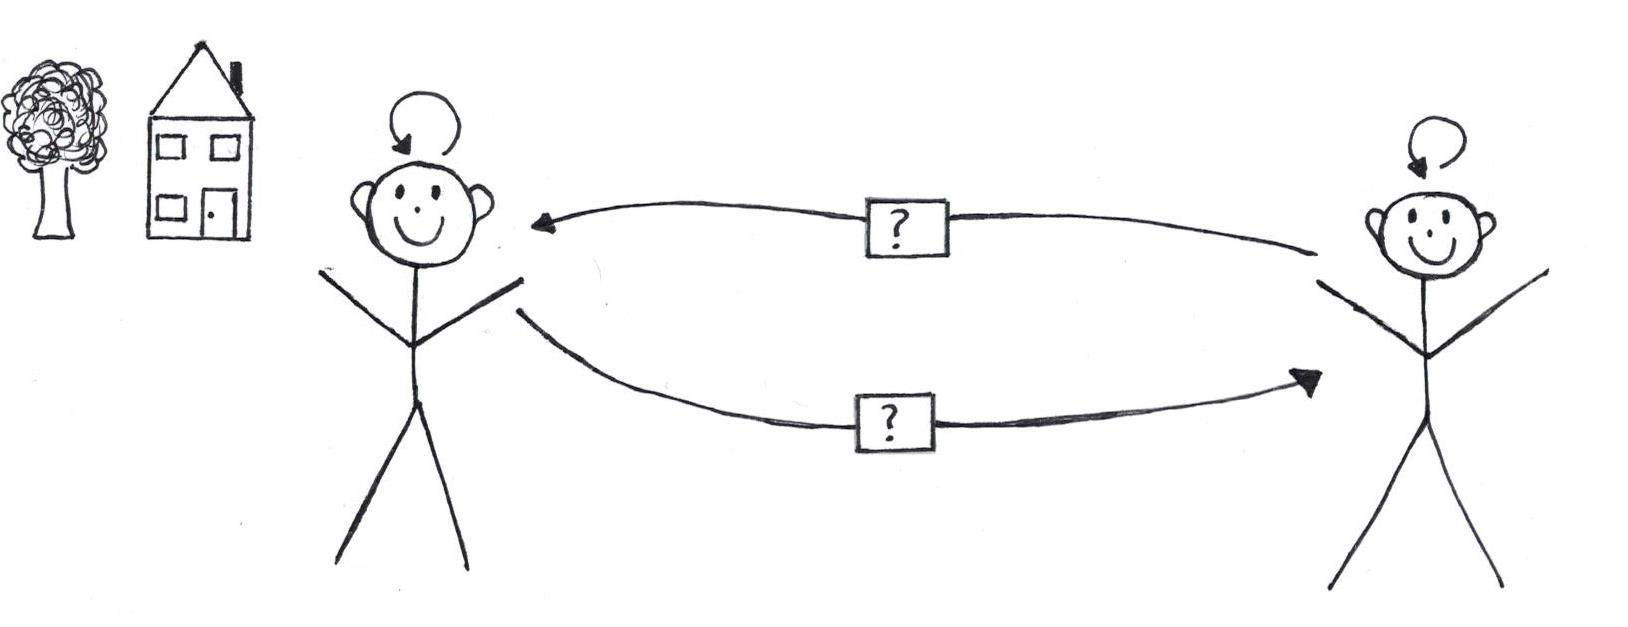
\includegraphics[width=0.6\textwidth]{grafiken/dialog/dialog}
\label{t5}
\end{center}
\end{figure}


\newpage
\section{Aufgabenstellungen}
1.	Was ist ein Turn? Recherchieren und notieren Sie eine Definition.
\vspace*{3cm}\\

2.	Suchen Sie in Ihren Aufnahmen nach Beispielen für Phrasierungen, die mit der Grammatik (syntaktische Phrase, Komma etc.) (a)  übereinstimmen und (b) von ihr abweichen.
\vspace*{3cm}\\
3.	Prüfen Sie in ihren Aufnahmen, ob Fragen mit einer steigenden oder anderen Grundfrequenz produziert werden.  Notieren Sie Beispiele und beschreiben sie den f0-Verlauf.
\vspace*{3cm}\\

4.	Bei welchen anderen Bereichen der Linguistik sehen Sie Schnittstellen mit der Prosodie und Intonation? Begründen Sie die Vorschläge.\vspace*{1cm}\\








\chapter{Abstrahieren} 

Bei der Analyse und Beobachtung artikulatorischer, akustischer und perzeptiver Aspekte gesprochener Sprache fällt die große Variabilität auf. Sprecher unterscheiden sich in ihrer Produktion (und folglich Akustik) von Sprachlauten und auch innerhalb eines Sprechers gibt es jede Menge Unterschiede: Kein Laut  wird jemals identisch produziert. Um die Funktion von Sprachlauten innerhalb einer Sprache und deren Lautinventar zu ermitteln, ist es nötig, die Variation auszuklammern und zu abstrahieren.

\section{Stichworte zur Vorlesung \em{Einführung in die Phonologie}}

Kontrast, Phon, Phonem, Allophon, freie Variante, komplementäre Distribution\dots $\rightarrow$ {\tt L8\underline{\ }Phonologie.pdf}

\begin{figure}[htbp]
\begin{center}
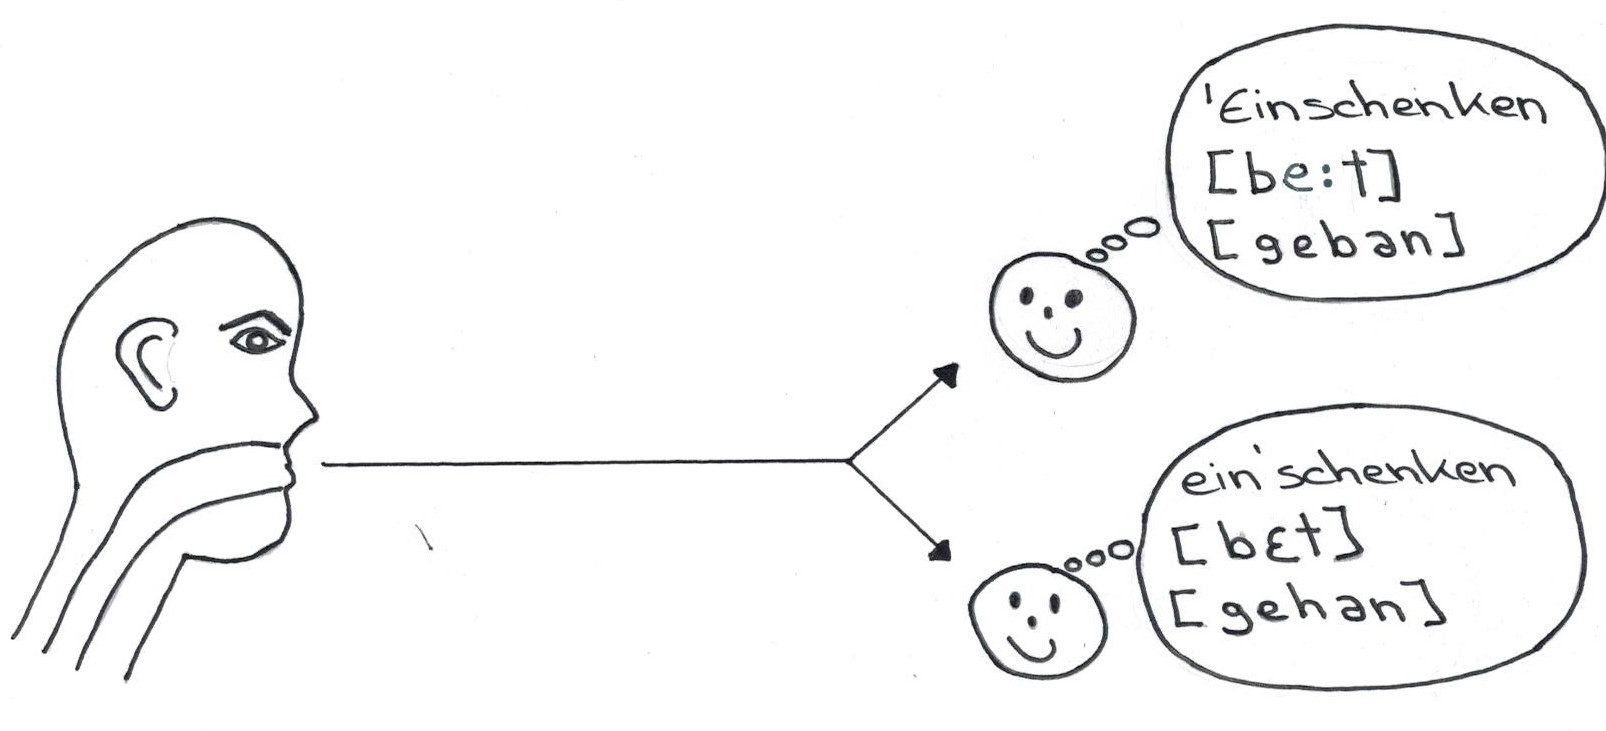
\includegraphics[width=0.6\textwidth]{grafiken/abstrahieren/distinktive-merkmale}
\label{t6}
\end{center}
\end{figure}




\newpage
\section{Aufgabenstellung}

1.	Lesen Sie den ausgeteilten Text von Trubetzkoy und stellen sie die ihrer Meinung nach wichtigsten Informationen schematisch dar.\vspace{\fill}


2.	Tragen Sie die Sprachlaute des Deutschen in folgende Tabelle ein und unterstreichen Sie alle Laute, die ihrer Meinung nach Phoneme des Deutschen sind.

\begin{sidewaystable}\centering
\small
\begin{tabular}{|l|l|l|lcr|l|l|l|l|l|l|}  \hline
 & Bilabial & Labiodental & Dental & Alveolar & Postalveolar & Retroflex & Palatal & Velar & Uvular & Pharyngeal & Glottal\\ \hline
Plosive	&	&	&	&	&	&	&	&	&	&	& \\ \hline
Nasal	&	&	&	&	&	&	&	&	&	&	& \\ \hline
Tap or Flap	&	&	&	&	&	&	&	&	&	&	& \\ \hline
Fricative	&	&	&	&	&	&	&	&	& 	&	& \\ \hline
Lateral fricative	&	&	&	&	&	&	&	&	&	&	& \\ \hline
Approximant	&	&	&	&	&	&	&	&	&	&	& \\ \hline
Lateral approximant	&	&	&	&	&	&	&	&	&	&	& \\ \hline


\end{tabular}
\end{sidewaystable}

\newpage
3.	Lesen Sie den ausgeteilten Text von Kohler. Ist der Glottalverschluss Ihrer Meinung nach ein Phonem des Deutschen? Notieren Sie Pro- und Contra-Argumente. \vspace{5cm}\\







\chapter{Spontansprachliche Vorgänge}

Auch wenn Spontansprache durch viel Variabilität charakterisiert ist, so sind viele spontansprachliche Vorgänge dennoch regelhaft. Diese lassen sich als phonologische Prozesse und Regeln beschreiben.

\section{Stichworte zur Vorlesung \em{Phonologische Prozesse und Regeln}}
Neutralisierung, Assimilation, Fortisierung/Lenisierung, Epenthese, Tilgung, Längung, Kürzung, Metathese, Reduplikation $\rightarrow$ {\tt L9\underline{\ }Spontansprache.pdf}

\begin{figure}[htbp]
\begin{center}
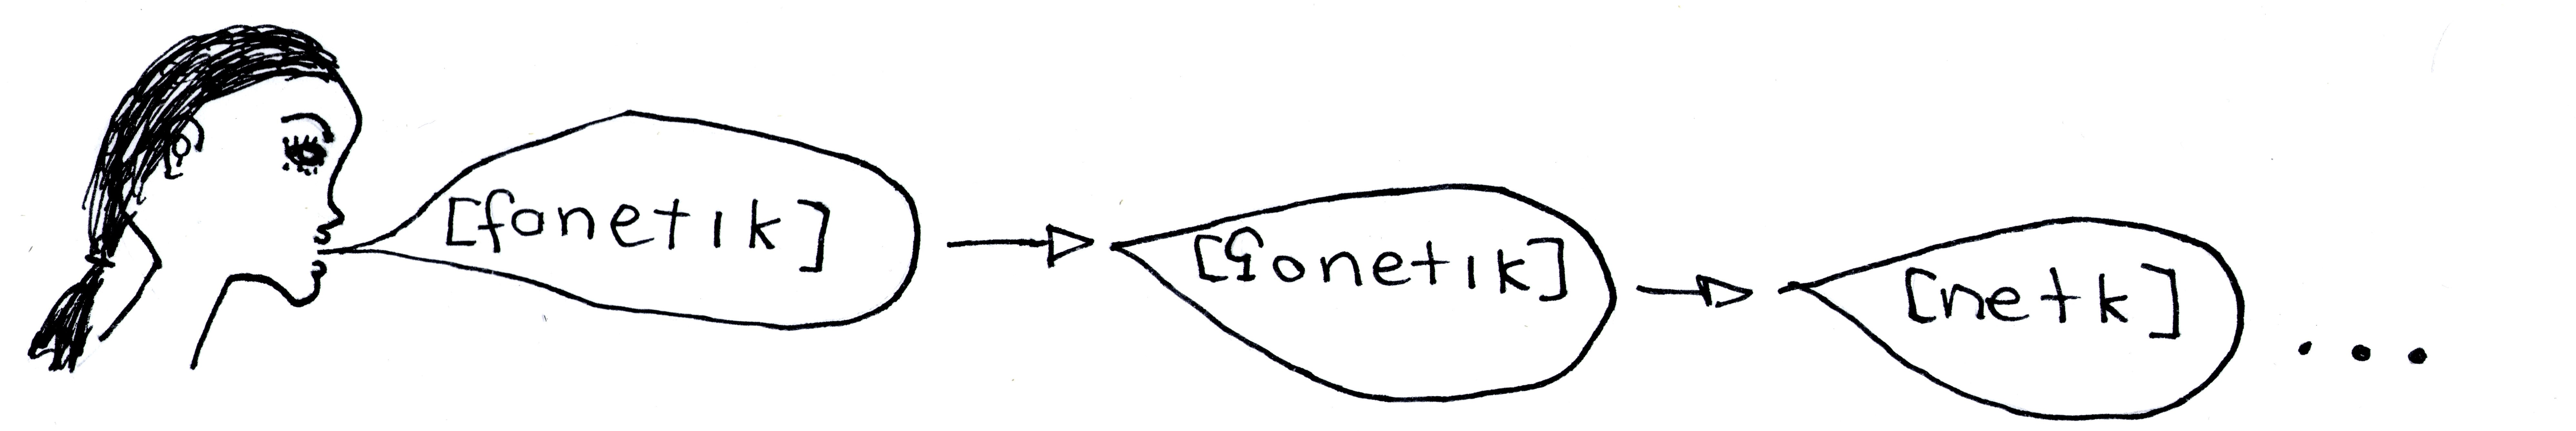
\includegraphics[width=\textwidth]{grafiken/spontansprachliche-vorgaenge/phonologische-prozesse}
\label{t7}
\end{center}
\end{figure}

\newpage
\section{Aufgabenstellungen}
1.	Identifizieren und erklären Sie die phonologischen Prozesse in den Daten:

\begin{center}
\begin{tabular} {|p{3cm}|p{3cm} |l|l|} \hline
peel [pi:l]&pool [p\super{w}u:l]\\ \hline
tea [ti:]&two [t\super{w}u:]\\ \hline
she [\textesh i:]&shoe [\textesh \super{w}u:]\\ \hline
leek [li:k]&Luke [l\super{w}u:k]\\ \hline
get [get]&got [g\super{w}ot]\\ \hline
\end{tabular}\vspace{1cm}\\
\end{center}

\begin{center}
\begin{tabular} {|p{3cm}|p{3cm} |l|l|} \hline
in-legal&illegal\\ \hline
in-licit&illicit\\ \hline
in-rational&irrational\\ \hline
in-revocable&irrevocable\\ \hline
in-possible&impossible\\ \hline
in-polite&impolite\\ \hline
in-patient&impatient\\ \hline
\end{tabular}
\end{center}




\chapter{Sprachdatenbanken}

\section{Einführung und Problemstellung}
%Definitionen, Ziele, Abgrenzung, verwandte Begriffe
%Topographie

Gesprochene Sprache ist höchst {\em variabel} und außerordentlich {\em reich an Information}. Abb. \ref{fig_sdb_strasse} zeigt zwei Äußerungen des Wortes 'Straße', gesprochen von zwei verschiedenen Personen.

\begin{figure}[htbp]
\begin{center}
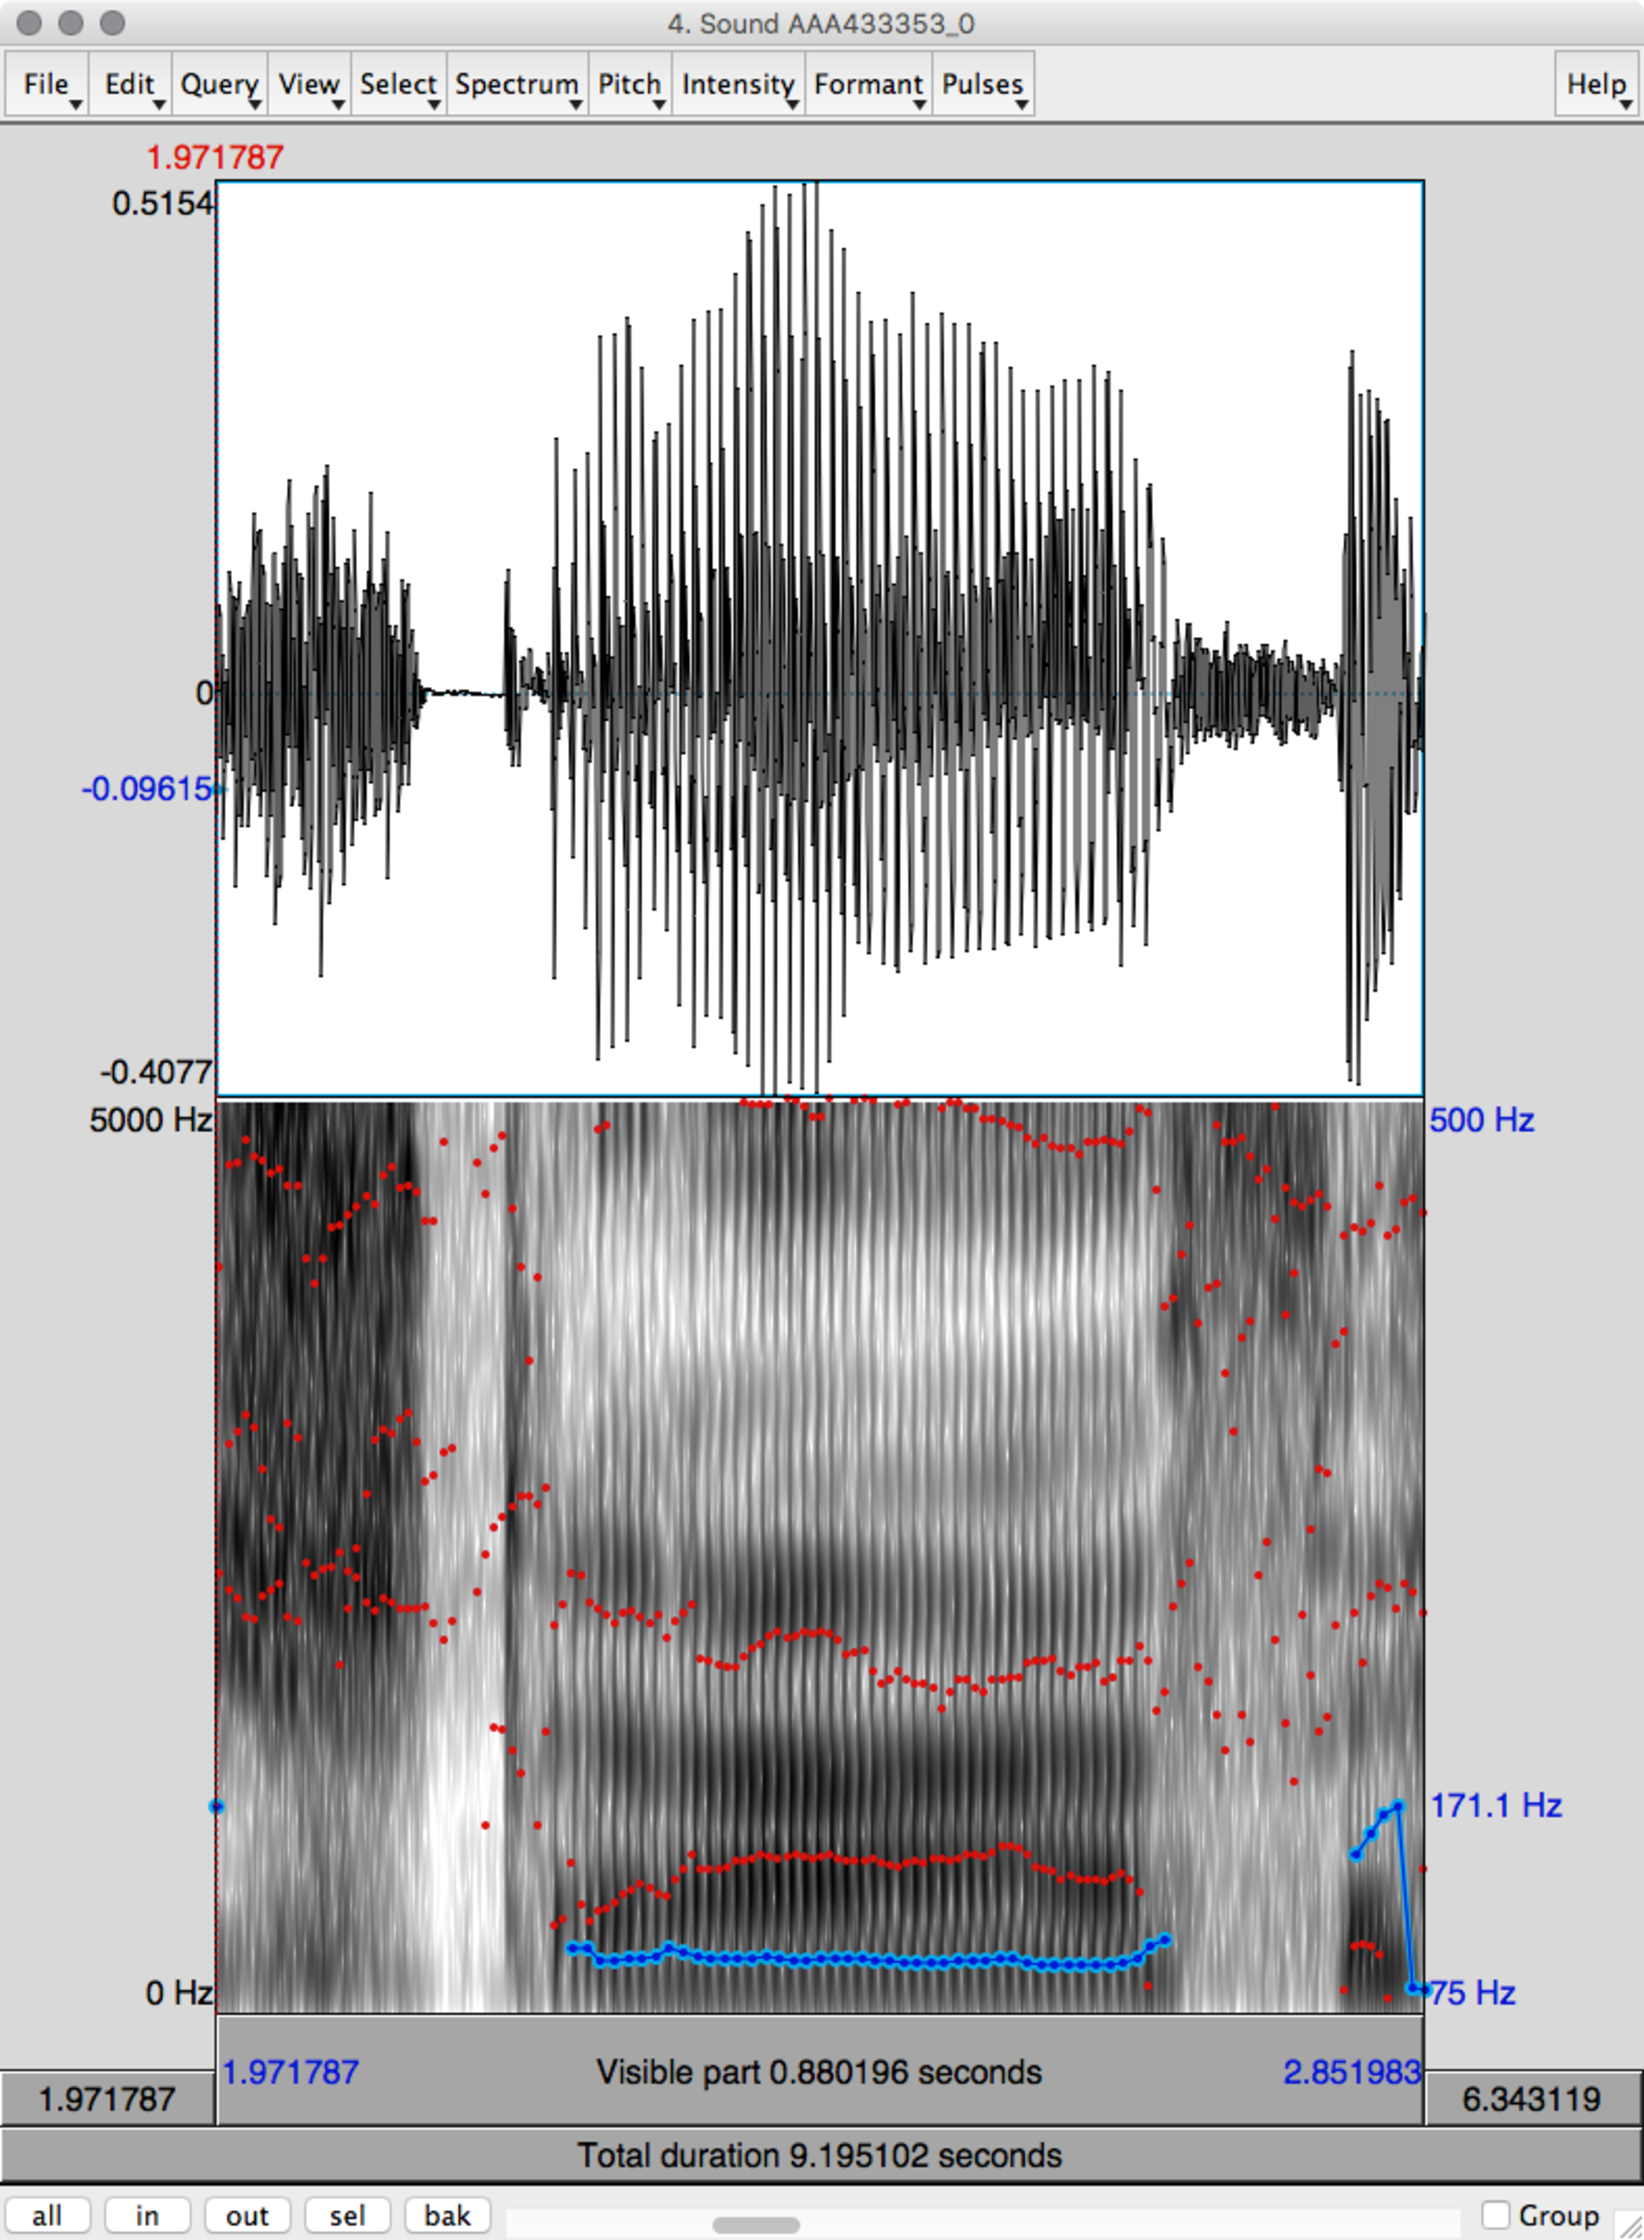
\includegraphics[width=.49\textwidth]{grafiken/sprachdatenbanken/STRASSE433353}
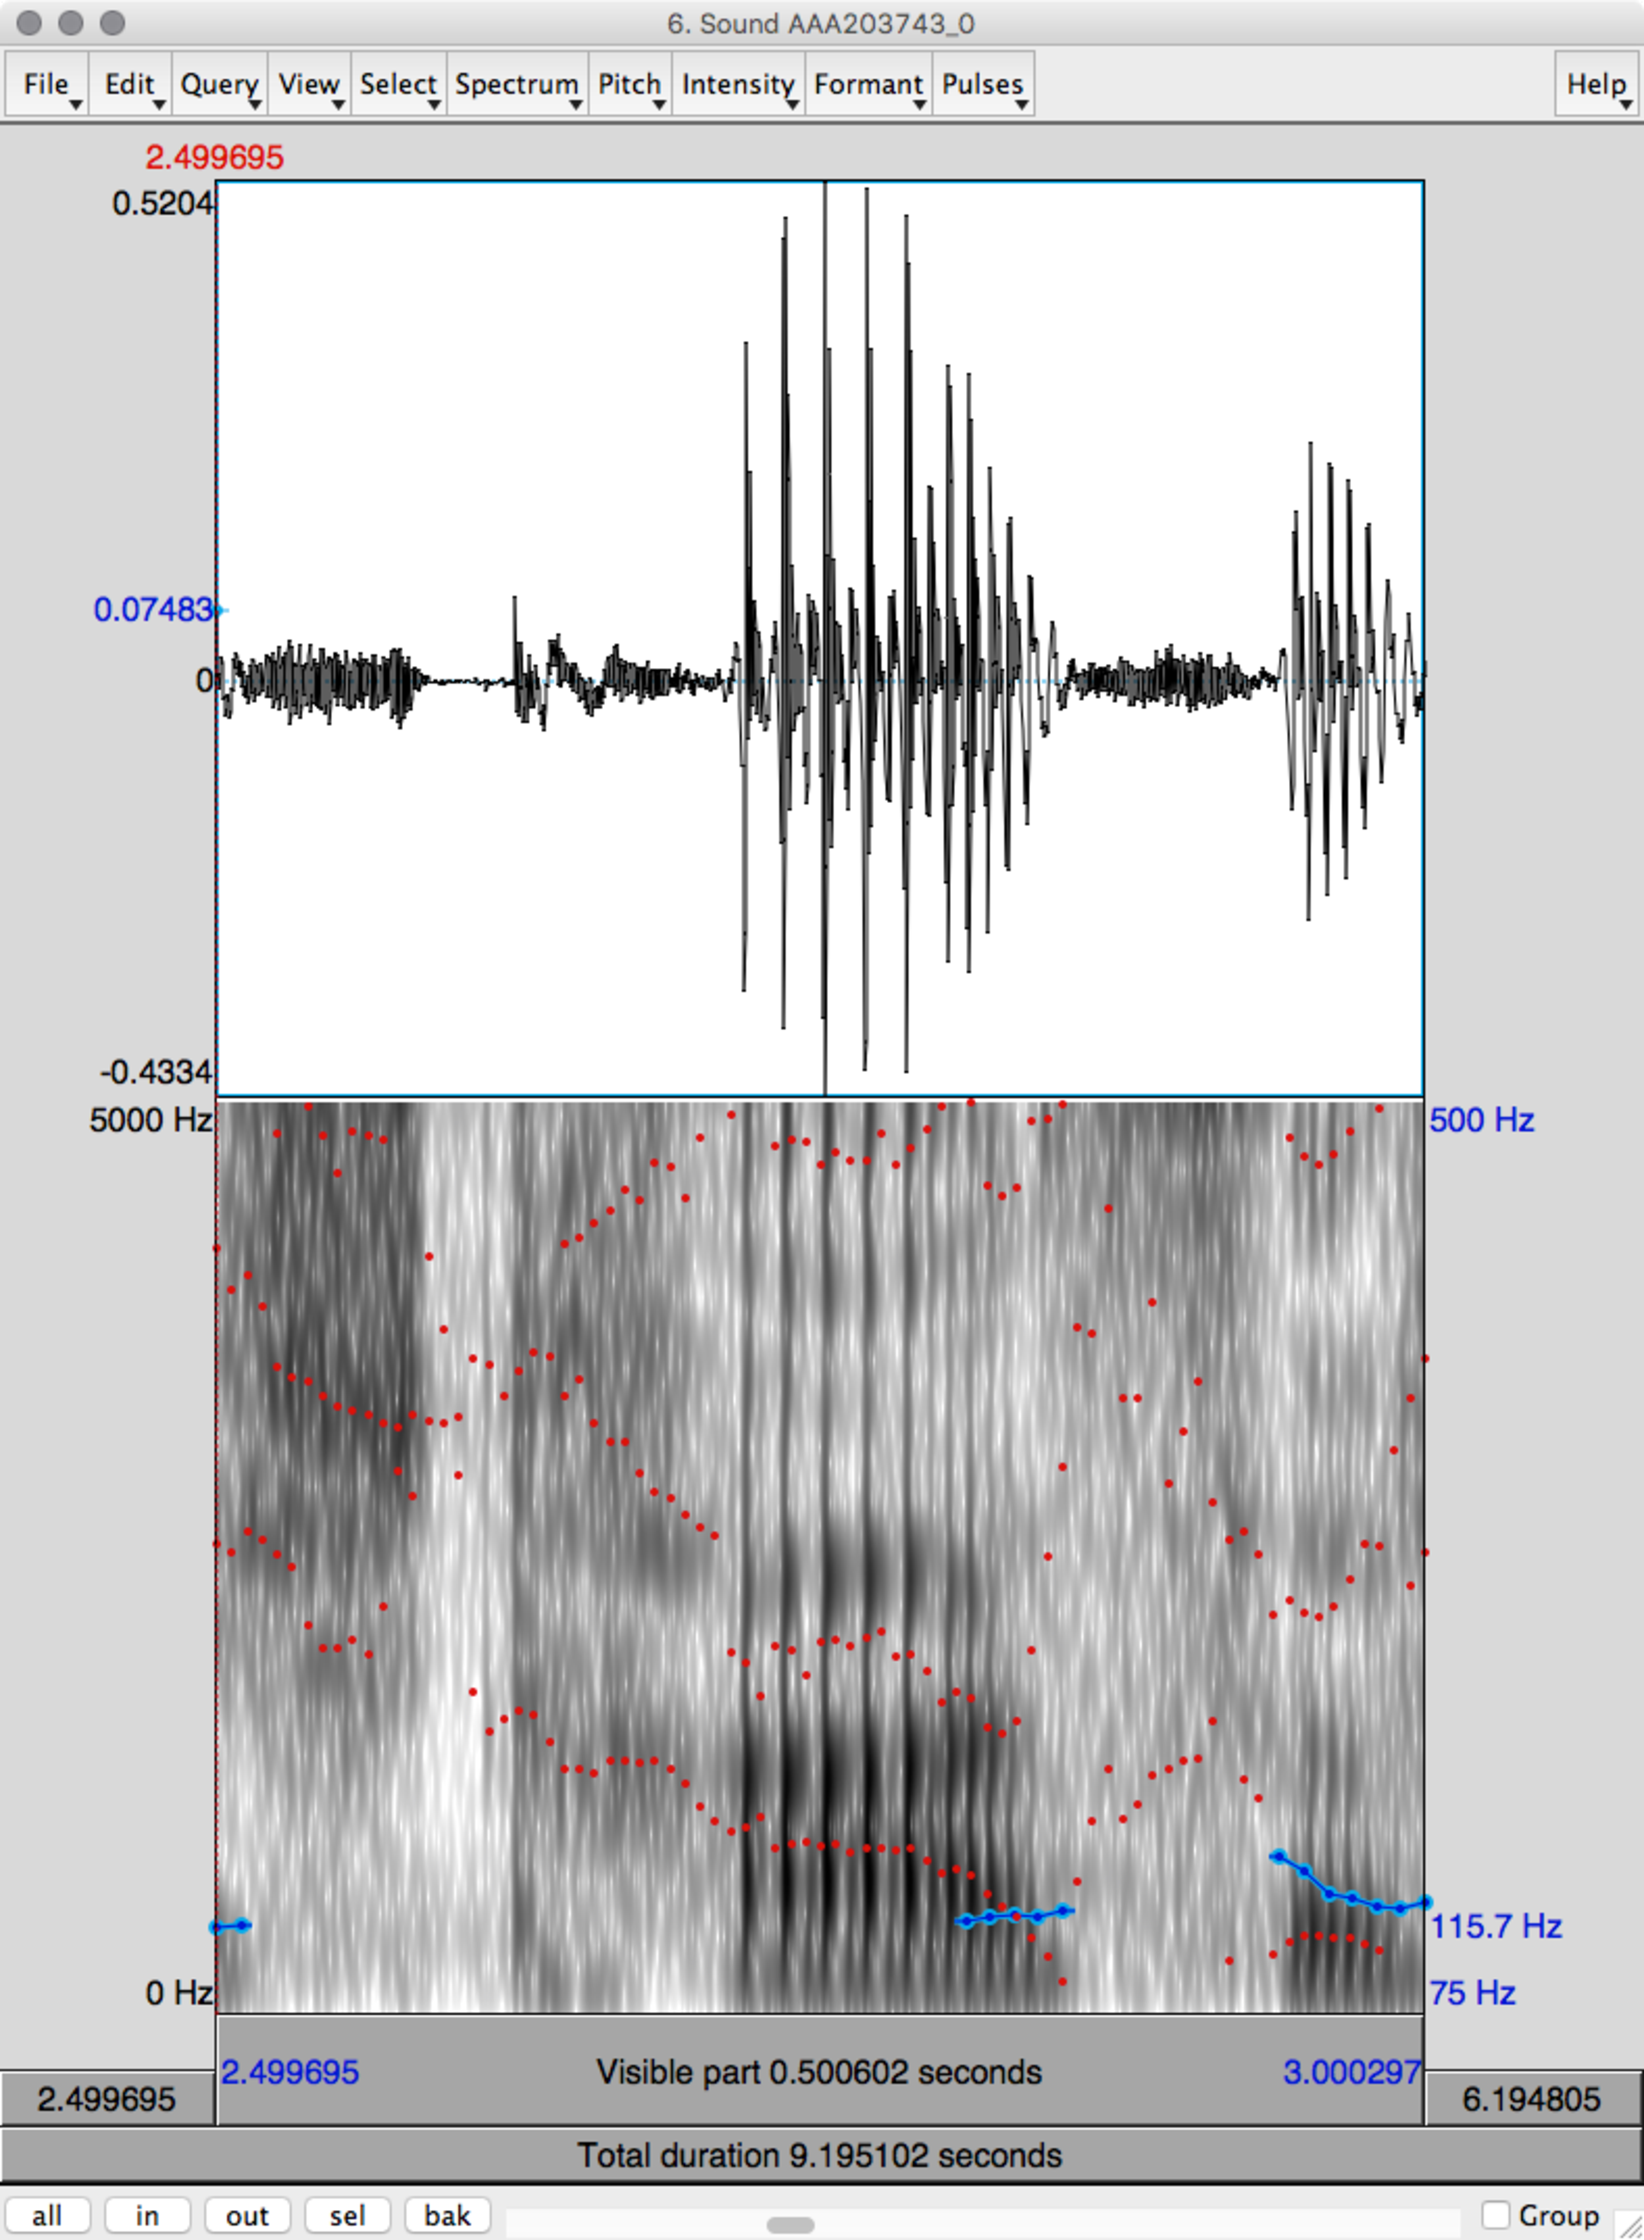
\includegraphics[width=.49\textwidth]{grafiken/sprachdatenbanken/STRASSE203743}
\caption{Das Wort 'Straße', gesprochen von einem Mann, 16 Jahre alt, 175 cm groß, aus Bayern (links) bzw. einem Mann, 17 Jahre alt, 183 cm groß, aus Sachsen (rechts)}
\label{fig_sdb_strasse}
\end{center}
\end{figure}

Bereits aus zwei so kurzen Äußerungen eines alltäglich vorkommenden Wortes können wir, allein durch Anhören, nicht nur das Wort selbst erkennen, sondern auch Aussagen zu Geschlecht, Alter und die regionale Herkunft der Sprecher, ja sogar zu ihrem Gesundheitszustand oder ihren Emotionen machen. 

Gesprochene Sprache ist {\em flüchtig} -- im Moment der Produktion ist sie bereits verflogen. Zur systematischen Untersuchung muss sie {\em persistent} gemacht werden. Sprachdatenbanken leisten genau dies: sie speichern gesprochene Sprache originalgetreu und dauerhaft, und sie stellen die gespeicherten Sprachsignale und Annotationen zur weiteren Verarbeitung zur Verfügung. Digitale Sprachaufnahmen können immer wieder abgespielt, übertragen, sichtbar gemacht und technisch analysiert werden. 

Im signalphonetischen Band gehören Sprachdatenbanken somit in den Bereich {\em Akustik}, sie stehen also zwischen Sprecher und Hörer. Sie sind ein {\em Zwischenspeicher}, der das akustische Signal und seine Annotation {\em archiviert}.

Die wissenschaftliche Fragestellungen im Kontext von Sprachdatenbanken lautet: Welche Daten muss man in welcher Qualität speichern? Welche fachlichen Aufgabengebiete können Sprachdatenbanken abdecken? Welche Abfragemöglichkeiten benötigt die Fachwissenschaft, um ihre inhaltlichen Fragestellungen bearbeiten zu können? Wie kann man sicherstellen, dass Sprachdaten langfristig verfügbar sind?

\section{Inhalte}
%Schwerpunkte, Methoden, ausgewählte Modelle
%Notizen, usw.

\subsection*{Definition} 
Eine {\em Sprachdatenbank} ist eine auf Dauer angelegte, explizit strukturierte und maschinenlesbare Sammlung von Daten gesprochener Sprache. 

Sie enthält die folgenden Arten von Daten:
\begin{description}
\item[Primärdaten]{Audio-, Video- oder Sensorsignaldaten von Sprechern oder Sprechvorgängen}
\item[Sekundärdaten]{Annotationen, d.h. Beschreibungen der Primärdaten}
\item[Metadaten]{Daten {\em über} die Primär- und Sekundärdaten, Dokumentation, Nutzungsvereinbarungen}
\end{description}

{\em Primärdaten} sind prinzipiell unveränderlich: einmal aufgenommen und geschnitten, werden sie nur noch aus technischen Gründen konvertiert oder auf neue Speichermedien migriert. Primärdaten werden erst wertvoll durch passende Sekundärdaten.

{\em Sekundärdaten} sind Beschreibungen des Inhalts der Primärdaten. Sie sind veränderlich, denn es kann beliebig viele Annotationen einer Sprachaufnahme geben, und diese Annotationen können korrigiert und erweitert werden. Die Sekundärdaten dienen dazu, gezielt auf Ausschnitte der Signaldaten zuzugreifen, um diese einer weiteren Bearbeitung zugänglich zu machen. 

{\em Metadaten} beschreiben Struktur und Inhalt einer Sprachdatenbank: Sprache, technische Angaben, Anzahl der Sprecher und Aufnahmedateien, Ort der Aufnahmen, usw. Sie dienen der schnellen Orientierung, ob eine Sprachdatenbank für eine bestimme Fragestellung überhaupt geeignet ist. In der Regel sind die Metadaten frei verfügbar, und sie bilden die Basis von Internetkatalogen zu Sprachressourcen. 

Beispiele von Sprachdatenbanken am Institut sind z.B. {\em CI\_1} mit Sprachaufnahmen von Cochlea-Implantat Patienten, oder {\em Ph@ttSessionz} mit Aufnahmen jugendlicher Sprecher und Sprecherinnen. Sie sind im CLARIN Repository zu finden (siehe \ref{link_clarin_repository}).

\subsection*{Verwandte Begriffe}
\begin{description}
\item[Korpus]{wird häufig synonym zu {\em Sprachdatenbank} verwendet, kann aber auch Sammlungen gesprochener Sprache bezeichnen, die
(noch) nicht in digitaler Form vorliegen. So definiert (Bussmann 1990) ein Korpus als: {\em endliche Menge von konkreten sprachlichen Äußerungen, die als empirische Grundlage für sprachwissenschaftliche Untersuchungen dienen.}}
\item[Repository]{ist eine im Web verfügbare, strukturierte Sammlung von Daten. Ein Repository bietet sowohl den Zugriff über eine grafische Nutzeroberfläche als auch eine Programmierschnittstelle an. In der Regel haben Nutzer nur lesenden Zugriff}
\end{description}

\subsection*{Theoretische Grundlagen}
Grundlage von Sprachdatenbanken ist, dass das Sprachsignal {\em physikalisch gemessen} werden kann, dass Sprachlaute {\em segmentale Einheiten} sind, und dass sich der sprachliche Inhalt aus der {\em sequenziellen Kombination} der Sprachlaute ergibt. Dazu ist ein {\em Kategorisierungsprozess} notwendig, der einzelnen Signalabschnitten Laute zuordnet, die mit Symbolen eines bestimmten Inventars, z.B. IPA Alphabet, bezeichnet werden (siehe Abb. \ref{fig_segmentation}).

\begin{figure}[htbp]
\begin{center}
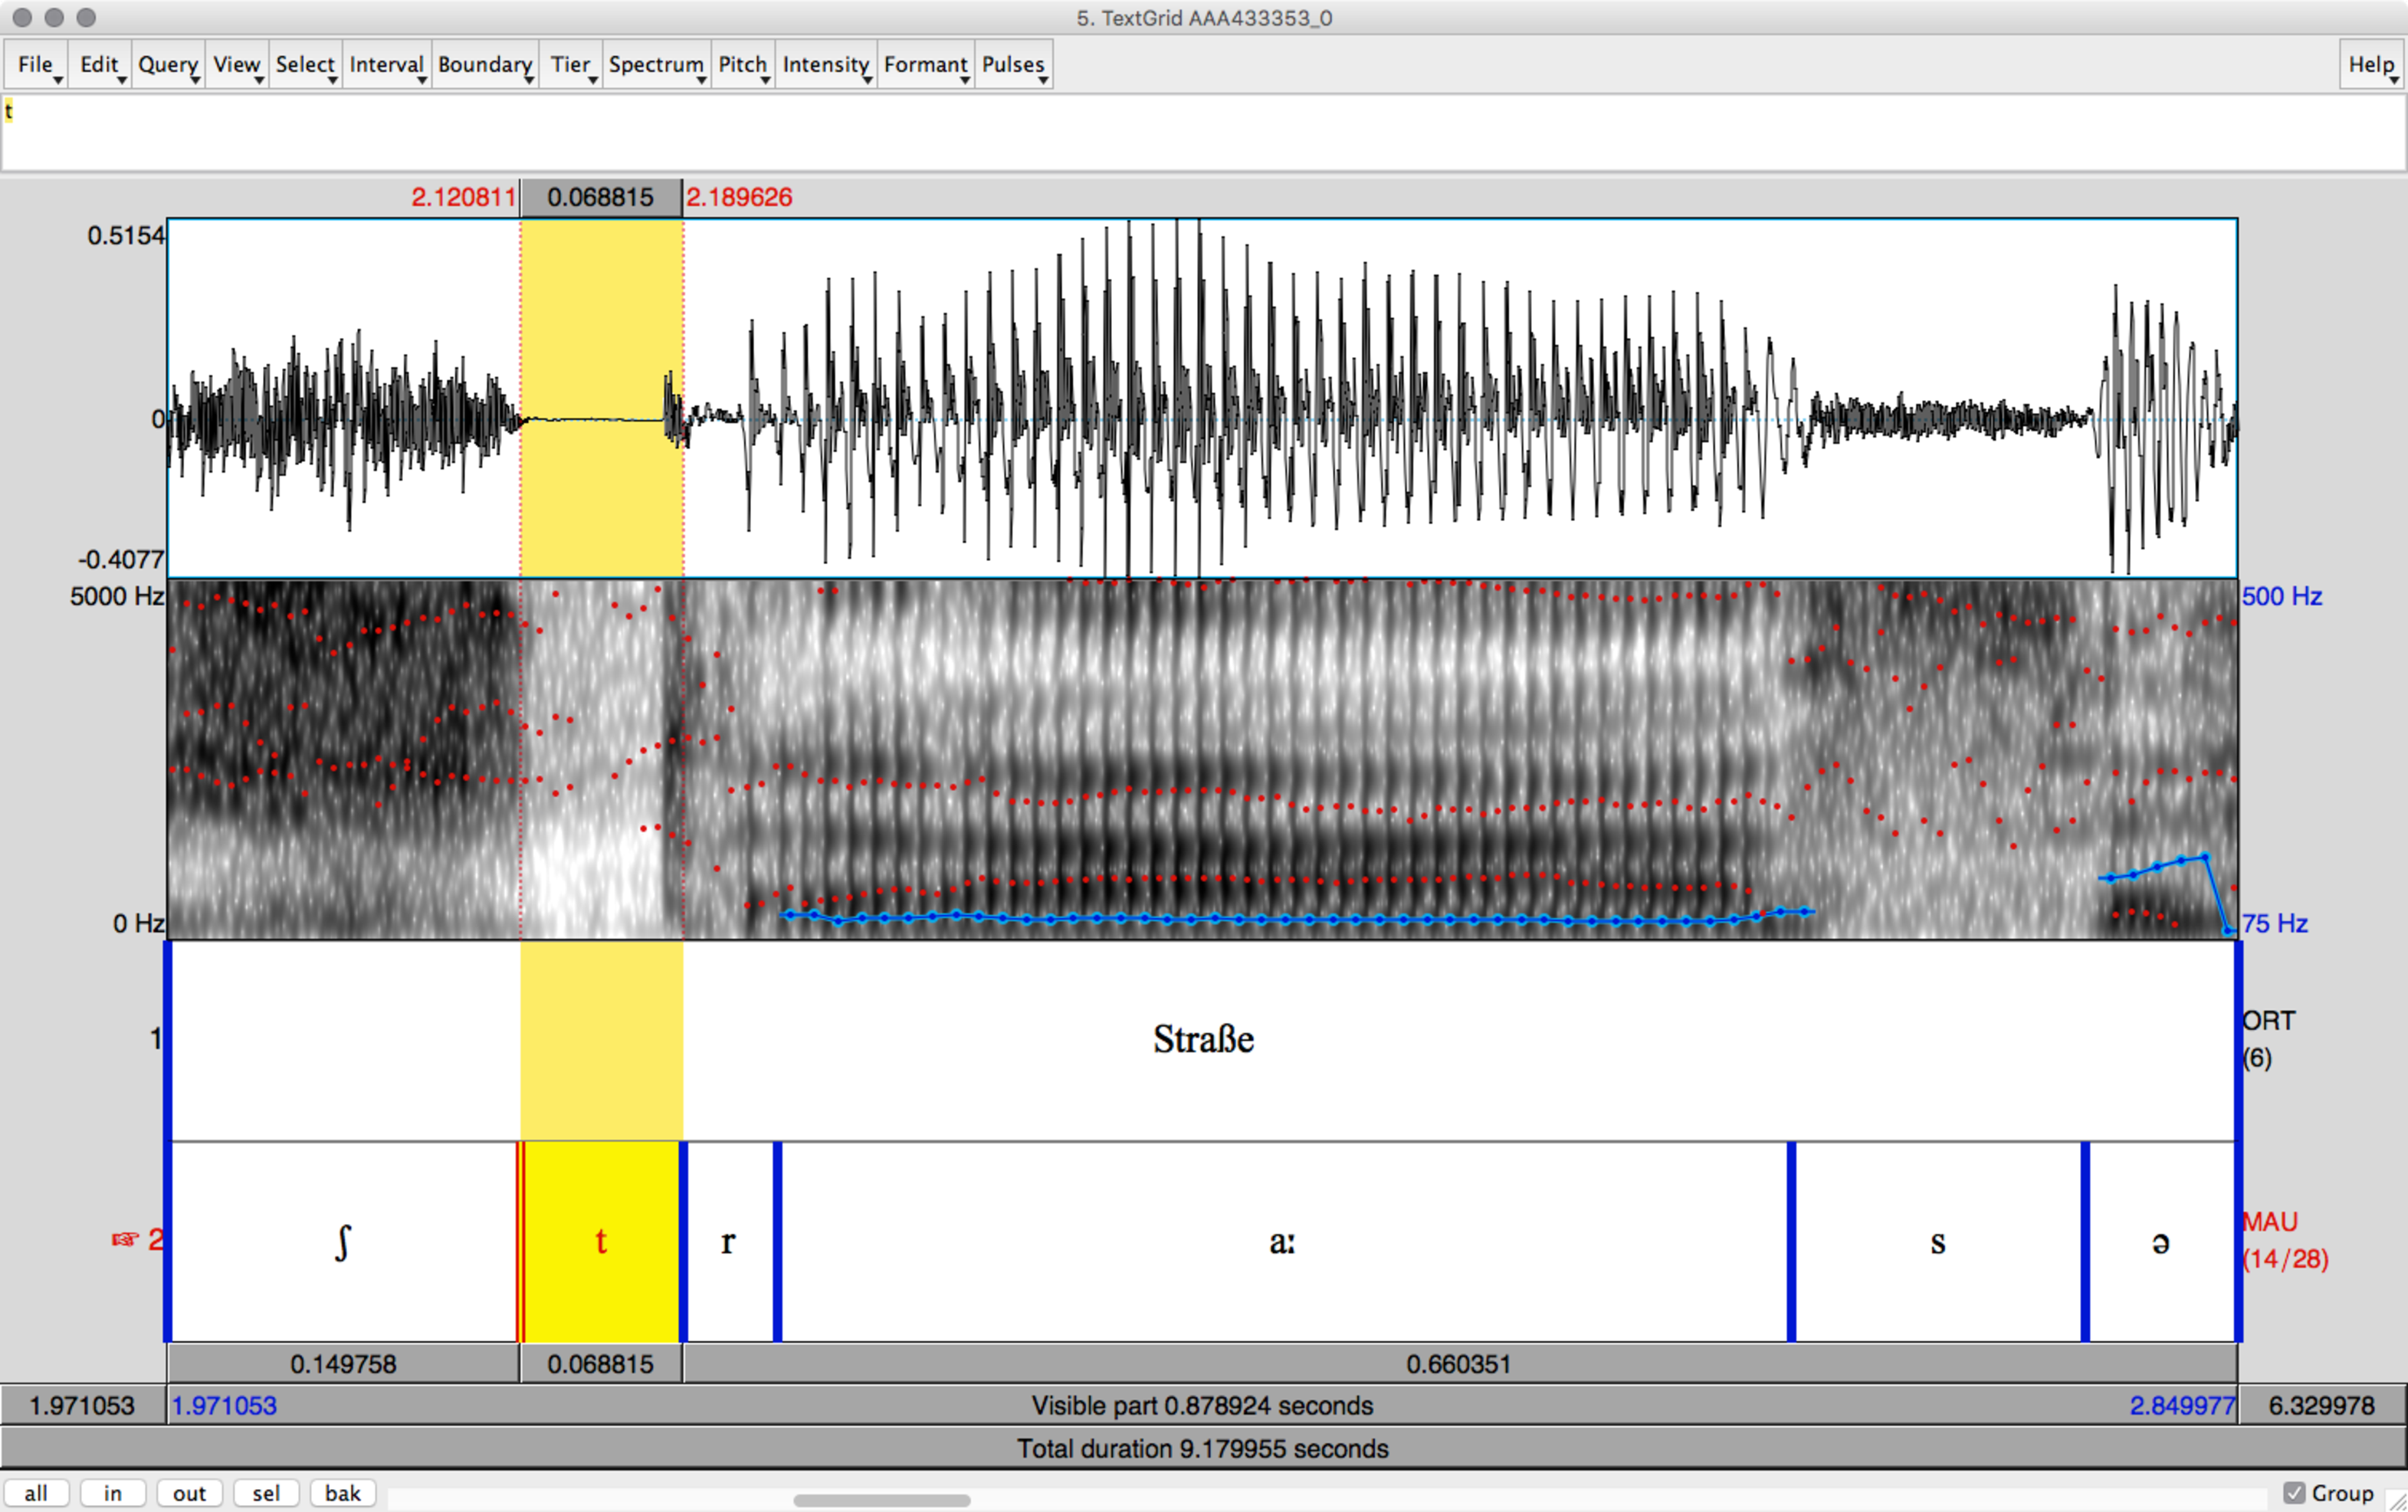
\includegraphics[width=1.0\textwidth]{grafiken/sprachdatenbanken/Segmentation}
\caption{Segmentiertes Sprachsignal mit den Annotationsebenen ORT (für Orhographie) und MAU (für automatisch segmentiert) des Wortes 'Straße'. Das Segment des Sprachlauts {\tt [t]} ist selektiert.}
\label{fig_segmentation}
\end{center}
\end{figure}

\subsection*{Digitale Daten}
Erst mit der digitalen Speicherung von Sprachdaten sind Sprachdatenbanken möglich geworden: sowohl Signal- als auch Annotationsdaten können maschinell verarbeitet, die Daten verlustfrei vervielfältigt werden. Die Daten können unbeschränkt verlustfrei kopiert und verteilt werden, es gibt eine große Vielfalt an Signal- und Annotationseditoren, Aufnahmeprogramme sowie Auswertungs- und Statistiksoftware.

\subsection*{Datenzentren}
Auf Sprachdaten spezialisierte Datenzentren wie die ELRA ({\em European Language Resources Association}), das LDC ({\em Linguistic Data Consortium}) und das BAS ({\em Bayerisches Archiv für Sprachsignale}) am IPS (Abb. \ref{fig_sdb_datenzentren}) stellen Sprachdatenbanken in Repositories zur Verfügung. Forschungsinfrastrukturen wie CLARIN bieten ein ermöglichen die parallele Suche verteilten Datenzentren, einen Austausch kompatibler Daten sowie ein einheitliches Login.

\begin{figure}[htbp]
\begin{center}
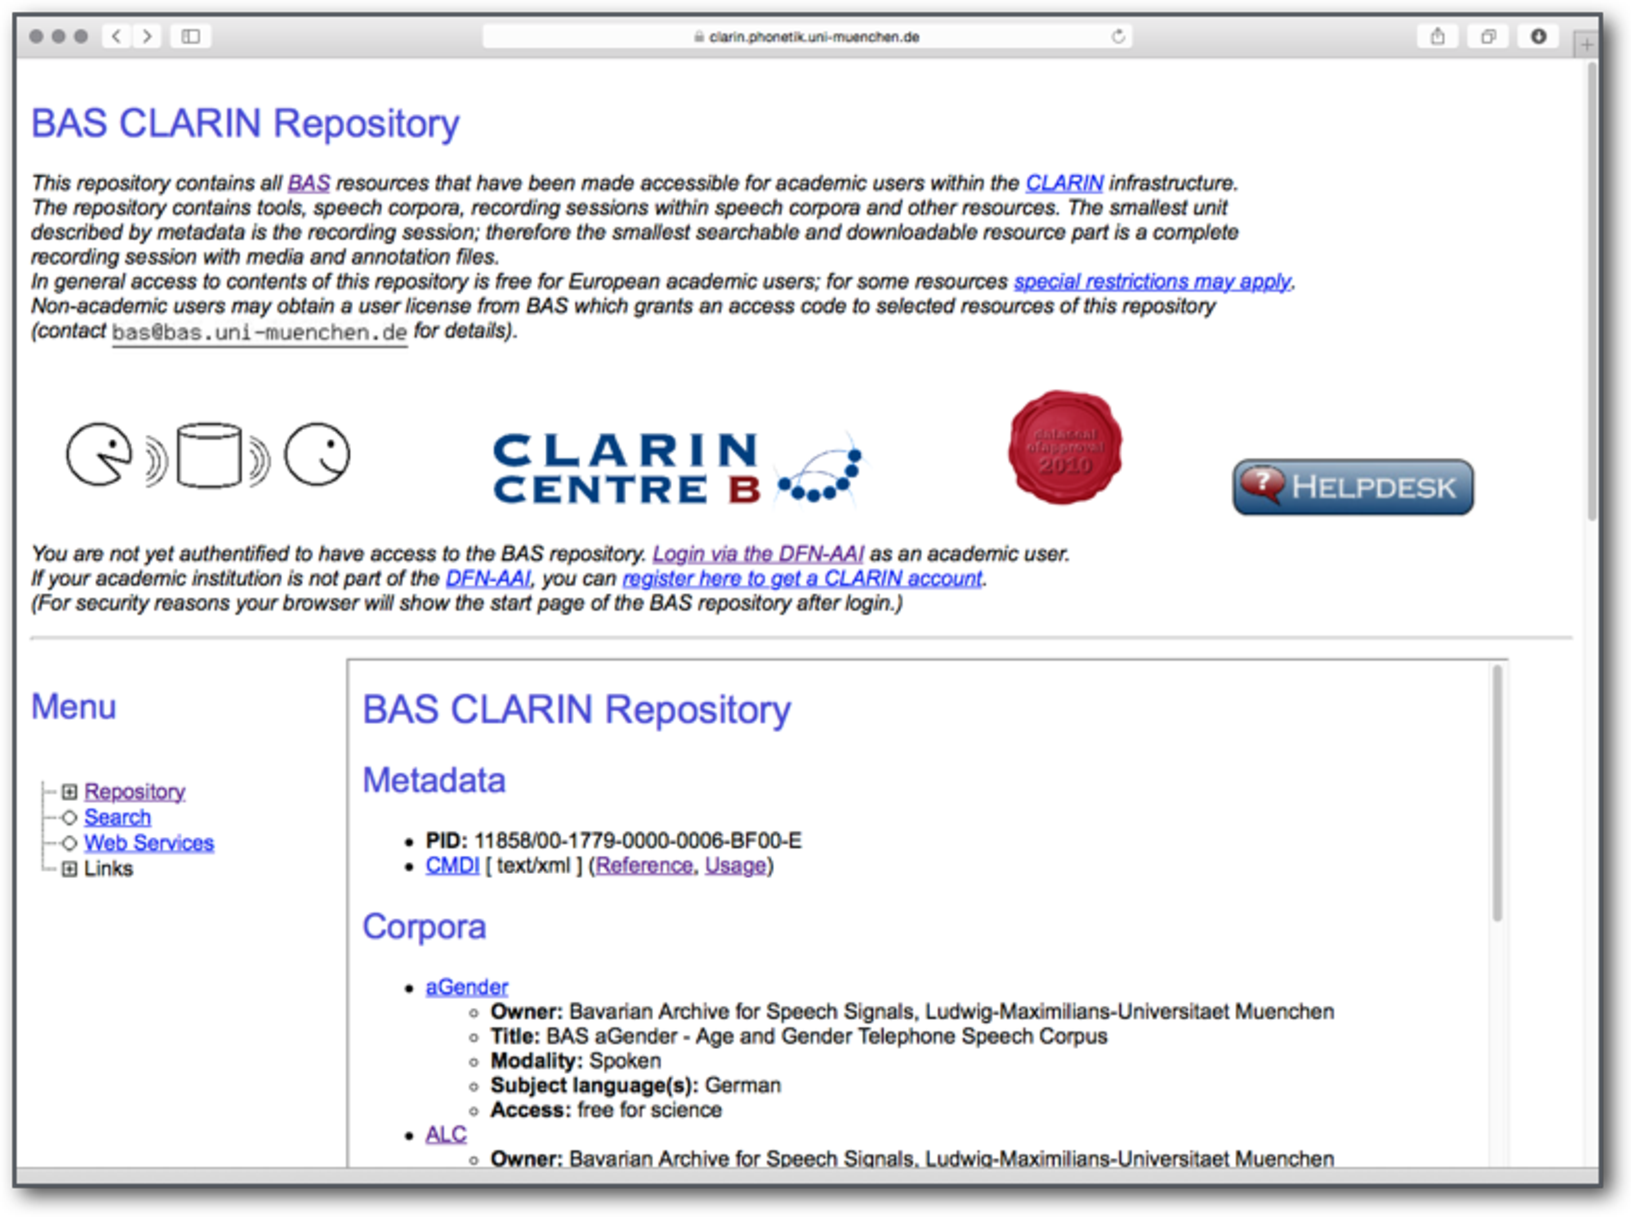
\includegraphics[width=1\textwidth]{grafiken/sprachdatenbanken/bas-repository}
\caption{CLARIN-D Repository des Bayerischen Archivs für Sprachsignale am IPS.}
\label{fig_sdb_datenzentren}
\end{center}
\end{figure}

\subsection*{Erstellung von Sprachdatenbanken}
Abb. \ref{fig_sdb_phasenmodell} stellt die Phasen und Arbeitsverteilung der Sprachdatenbankerstellung dar. Die in dieser Abbildung getrennten Rollen Auftraggeber ({\em extern}) und Ausführender ({\em intern}) können auch zusammenfallen.

\begin{figure}[htbp]
\begin{center}
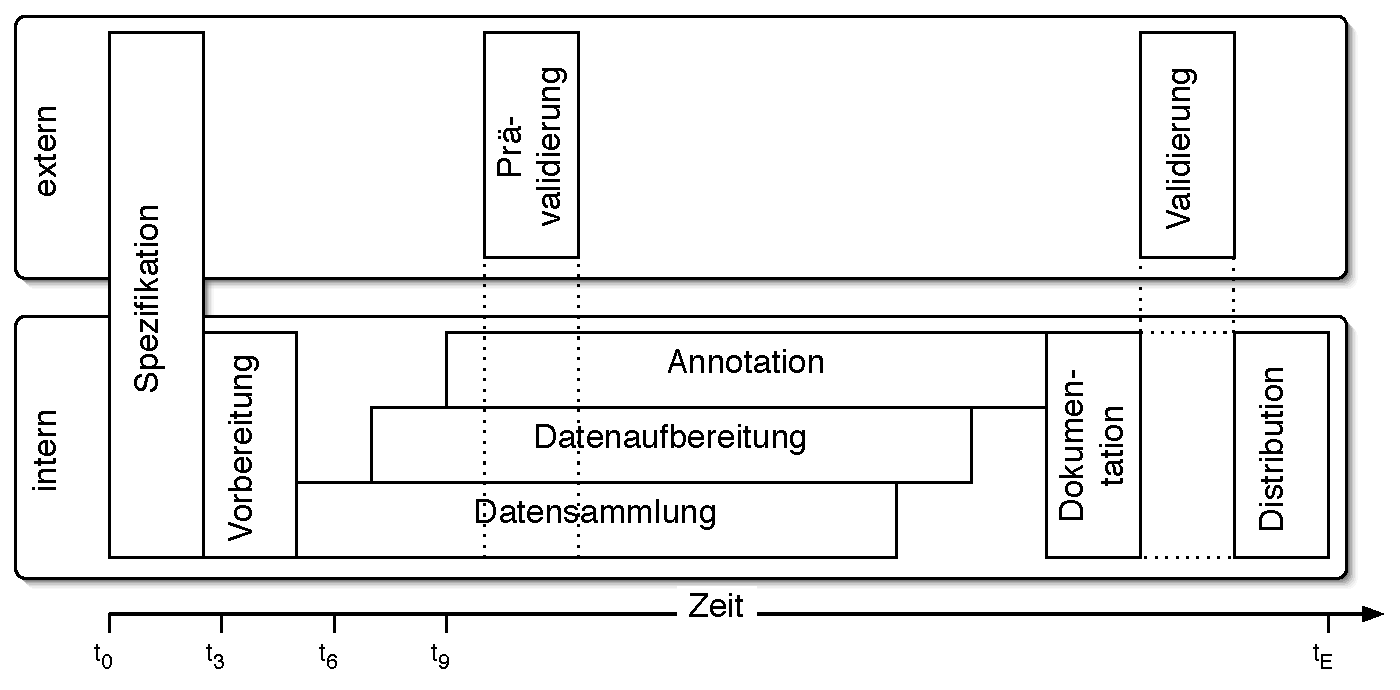
\includegraphics[width=1\textwidth]{grafiken/sprachdatenbanken/corpus-phasemodel-de}
\caption{Phasenmodell für die Erstellung von Sprachdatenbanken}
\label{fig_sdb_phasenmodell}
\end{center}
\end{figure}


\subsection*{Arbeitsablauf und Tools}
Zur Erstellung von Sprachdatenbanken verwendet man eine Reihe von Softwarewerkzeugen ({\em Tools}), die jeweils unterschiedliche Daten verarbeiten bzw. erstellen.

\begin{figure}[htbp]
\begin{center}
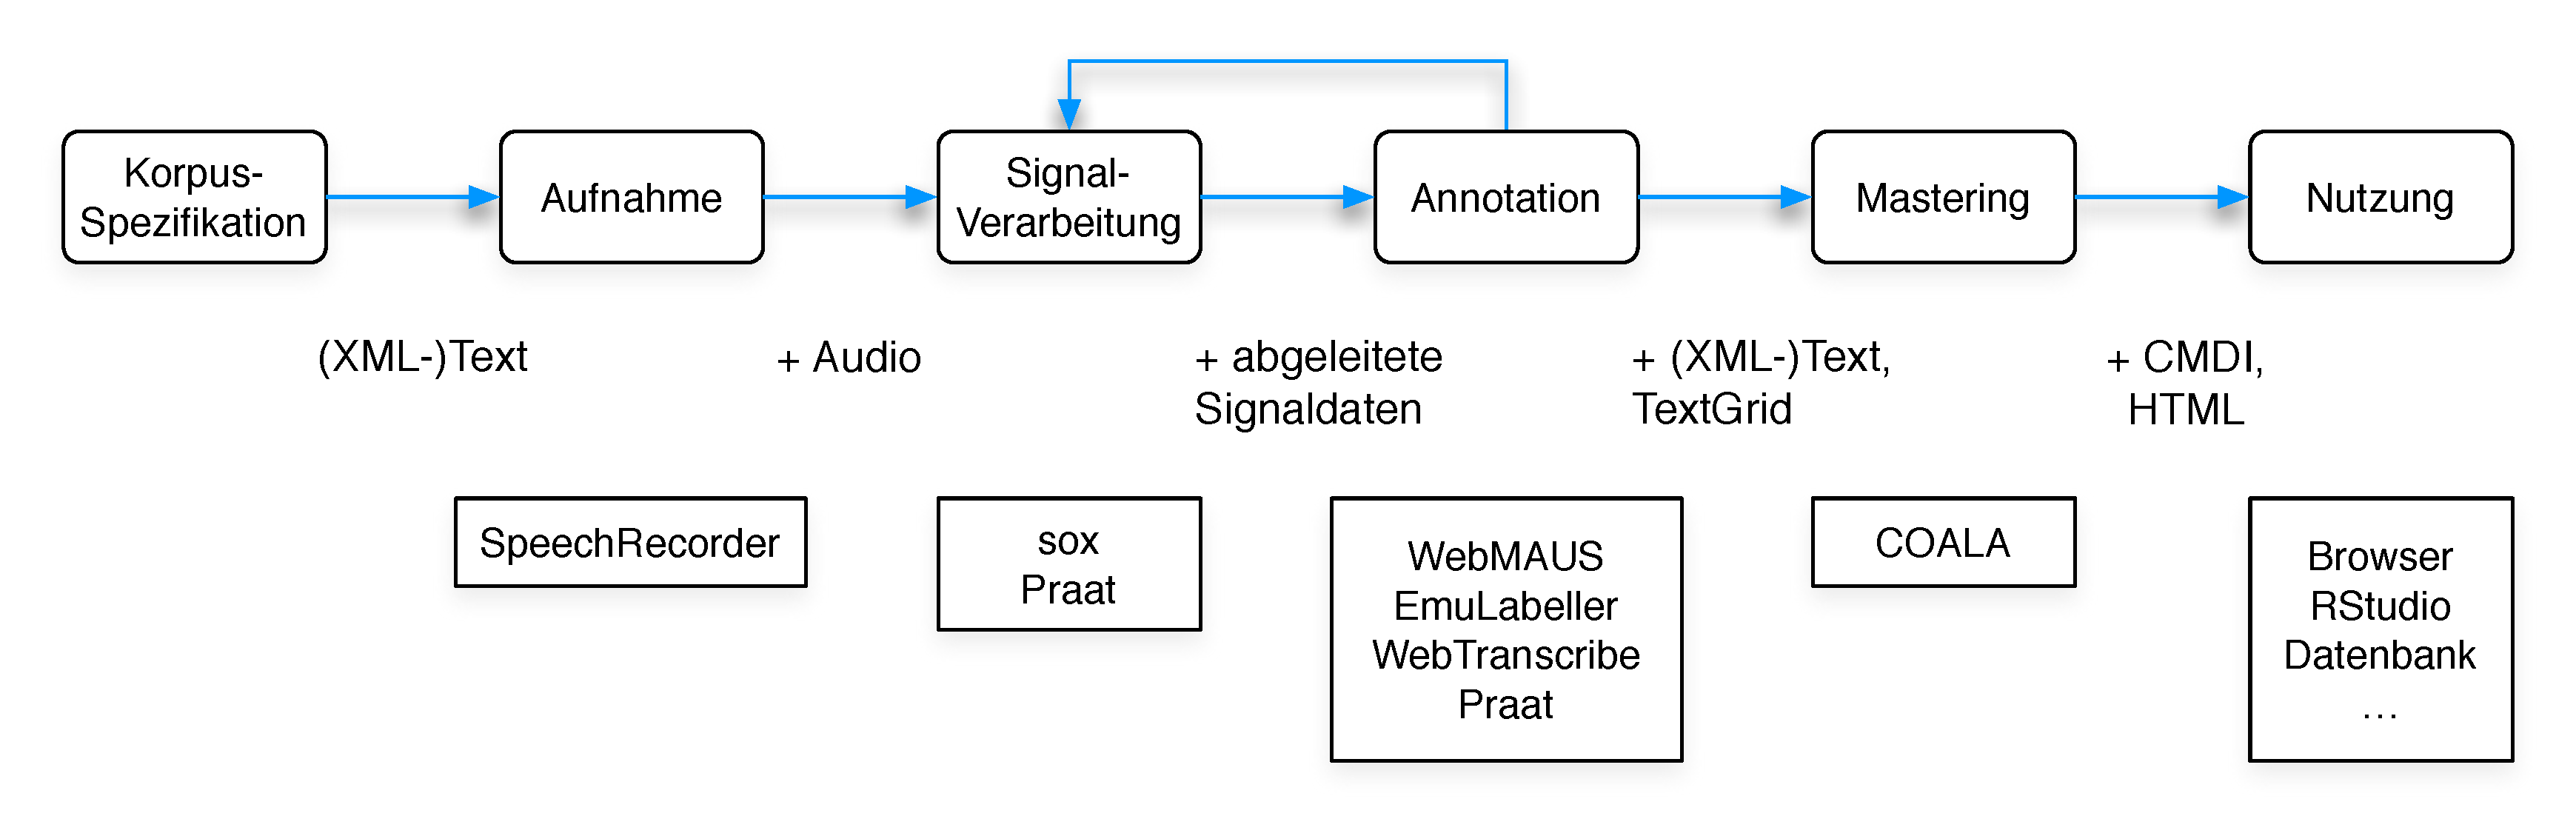
\includegraphics[width=1\textwidth]{grafiken/sprachdatenbanken/workflow-de-2}
\caption{Arbeitsablauf und Daten bei der Erstellung und Nutzung von Sprachdatenbanken. In den Kästchen stehen die Namen von Tools, die in diesem Arbeitsschritt häufig verwendet werden.}
\label{fig_sdb_arbeitsablauf}
\end{center}
\end{figure}

\subsection*{Sprachdatenbank Ph@ttS
essionz}
Die Sprachdatenbank Ph@ttSessionz wurde ursprünglich zur Verbesserung von Spracherkennungssystemen für die Stimmen Jugendlicher erstellt. Da sie aber Aufnahmen aus allen Regionen Deutschlands sowie Informationen über den Ort der Einschulung der Sprecher enthält, kann sie auch für die Untersuchung regionaler Varietäten des Alltagsdeutschen verwendet werden.

\begin{itemize}
\item{Sprachdatenbank ursprünglich zur Technologieentwicklung}
\item{jugendliche Sprecher (Alter 12-20)}
\item{46 Aufnahmeorte in Deutschland}
\item{1019 Sprecher, 130.060 Äußerungen}
\item{orthographische Transkription}
\item{automatisch phonetisch segmentiert}
\end{itemize}

\subsection*{Ph@ttSessionz: ein Anwendungsbeispiel}
Aus den Daten über die Sprecher sowie den Signaldateien der Sprachdatenbank Ph@ttSessionz kann man die Veränderung der Stimmhöhe, oder, phonetisch ausgedrückt, der {\em Grundfrequenz} oder {\em f0} bei Jugendlichen dokumentieren (siehe Abb. \ref{fig_sdb_grundfrequenz}). 
\begin{figure}[htbp]
\begin{center}
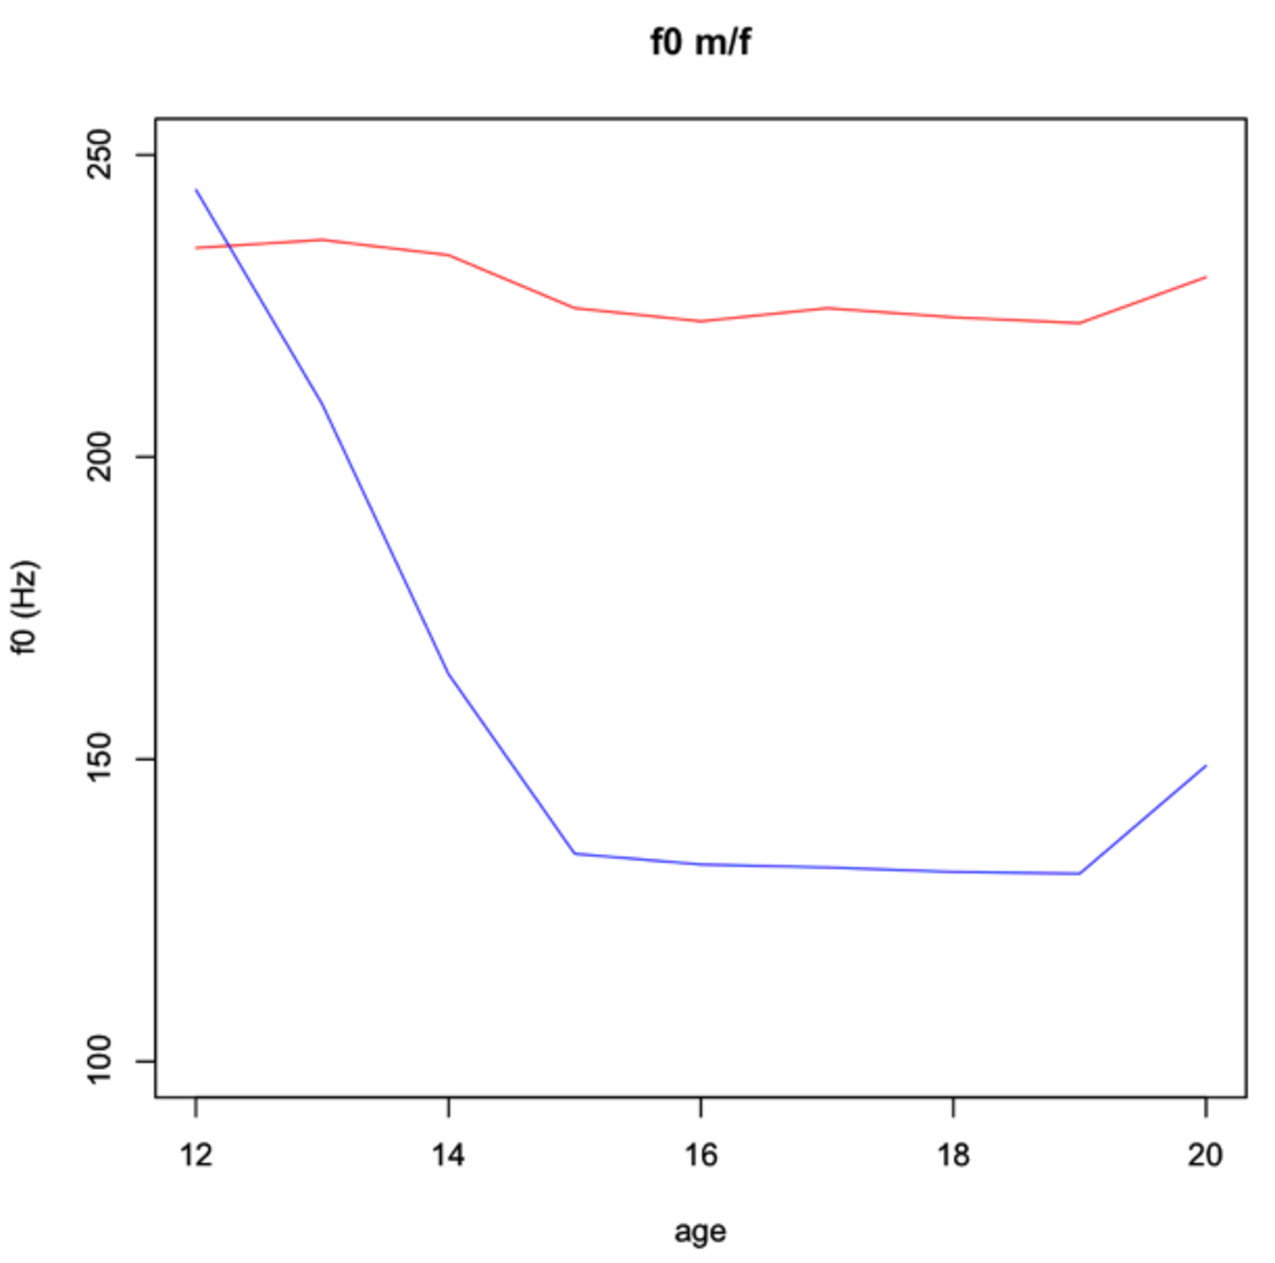
\includegraphics[width=0.8\textwidth]{grafiken/sprachdatenbanken/f0-entwicklung-phatt}
\caption{Diagramm der Veränderung der Grundfrequenz bei Jugendlichen, berechnet aus den Aufnahmen der Ph@ttSessionz-Sprachdatenbank}
\label{fig_sdb_grundfrequenz}
\end{center}
\end{figure}

%\newpage
%\section{Notizen}
%\newpage
\section{Übungen, Aufgaben}

\begin{enumerate}
\item{Nennen Sie drei der vier definierten Zeitalter phonetischer Datenerhebung}
\vspace{2cm}
\item{Welche Vorteile bieten web-basierte Sprachaufnahme und -annotation gegenüber traditionellen Verfahren?}
\vspace{2cm}
\item{Warum ist im Diagramm des Arbeitsablaufs (Abb. \ref{fig_sdb_arbeitsablauf}) ein Rückwärtspfeil von Annotation zu Signalverarbeitung?}
\vspace{2cm}
\item{Sind Sekundärdaten erweiterbar oder veränderbar? Wenn ja, wieso?}
\vspace{2cm}
\end{enumerate}


\section{Verknüpfungen im Fach} 
\begin{itemize}
\item{Sprachdatenbanken werden zum Trainieren von Sprach-, Sprachen- und Sprechererkennungssystemen benötigt, und sie bilden die Basis der konkatenativen Sprachsynthese.}
\item{Der Zugriff auf Sprachdatenbanken erfordert Abfragesprachen, die zu den Programmiersprachen zählen. Anwendungsprogramme und grafische Nutzeroberflächen nutzen Programmierschnittstellen, um die Inhalte der Datenbank zu verwenden. Um Daten in einer Sprachdatenbank ablegen zu können sind häufig Datenkonversionen notwendig, die mit Skripten programmiert werden.}
\item{Statistische Untersuchungen benötigen für die Beantwortung der Fragestellung geeignete Sprachdaten -- sowohl Signal- als auch Annotationsdaten -- in ausreichend großem Umfang.}
\item{Die Experimentalphonetik erhebt Sprachdaten. Diese werden als strukturierte Datenbestände in Sprachdatenbanken abgelegt, um dauerhaft und für unterschiedliche Untersuchungen zugänglich zu sein.}
\item{Die kognitive Sprachverarbeitung benötigt für empirische Untersuchungen, vor allem im Bereich perzeptiver Analysen, Signal- und Annotationsdaten aus Sprachdatenbanken.} 
\end{itemize}

\section{Literatur}

Bird, S.; Liberman, M. (2001). A Formal Framework for Linguistic Annotation. Speech Communication Band 33 Nr. 1,2. S.\,23-60. \newline\\
Bussmann, H. (1990). Lexikon der Sprachwissenschaft. Stuttgart: Körner Verlag.\newline\\
Draxler, C. (2008). Korpusbasierte Sprachverarbeitung. Tübingen: Narr Verlag. \newline\\
Schiel, F.; Draxler, C.; Baumann, A.; Ellbogen, T.; Steffen, A. (2003). The Production of Speech Corpora. Institut für Phonetik. LMU München.\newline\\
Schiel, F. (2003). The Validation of Speech Corpora. Institut für Phonetik. LMU München.


%\section{Links}
\label{link_clarin_repository}
{\tt clarin.phonetik.uni-muenchen.de/BASRepository/} (Stand: \today) Repository des Bayerischen Archivs für Sprachsignale am Institut für Phonetik der LMU.\newline\\
{\tt www.clarin.eu/content/virtual-language-observatory} (Stand: \today) Facettensuche nach Sprachdatenbanken.\newline\\
{\tt ldc.upenn.edu} (Stand: \today) Linguistic Data Consortium an der Universität von Pennsylvania.\newline\\
{\tt catalog.elra.info} (Stand: \today) Online Katalog der European Language Resources Asscociation.\newline\\
{\tt wals.info} (Stand: \today) World Atlas of Linguistic Structures online zur Dokumentation von Sprachstrukturen.








\chapter{Automatische Spracherkennung}

\section{Übersicht}

{\bf Versuch einer Definition}
%Kursiv geändert
Automatische Spracherkennung (automatic speech recognition, ASR) 
ist die technische (d.\,h. ohne menschliche 
Hilfe) Abbildung des physikalischen 
(messbaren) Sprachsignals auf Symbole, deren semantischer Gehalt nach 
dem Konsens der jeweiligen Sprachgemeinschaft f\"ur dieses Signal 
stimmig ist. Diese Symbole
k\"onnen linguistischer Natur sein (Laute, Silben, W\"orter...), 
aber auch logische, welche eine gew\"unschte 
Aktion ausl\"osen (z.\,B. An/Aus).

{\bf Verwandte Begriffe}
\begi
\item Sprachenerkennung (language recognition)
\item Sprechererkennung (speaker recognition)
\ndit

{\bf Blockschaltbild}

%\begin{figure}
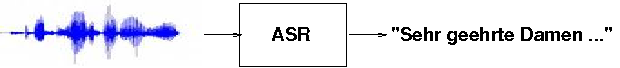
\includegraphics[width=\textwidth]{grafiken/automatische-spracherkennung/block.png}
%\caption{} \label{}
%\end{figure}

{\bf Problem: Warum l\"a{\ss}t sich diese Abbildung nicht programmieren?}
\begi
\item Sprachsignale sind extrem variabel: keine gesprochene \"Au{\ss}erung kann
exakt gleich wiederholt werden.
\item Stimmen verschiedener Sprecher unterscheiden sich
\item Zeitliche Dynamik: Beginn und Ende linguistischer Einheiten nicht erkennbar
\item Akustik: Abstand zum Mikrophon und Reflektionen
\item St\"orger\"ausche
\ndit

\section{Störparameter} 

Mensch:  Stimmung, Geschwindigkeit, gesundh. Zustand,
                 Erschöpfung, kooperativ/n. kooperativ,
                 Lombard-Effekt.\\
Akustik: Wechselnde Umgebung (Echo/Hall), Hintergrund-
                 geräusche, Abstand zum Mikrofon.\\
Mikrofon: Versch. Charakteristik, Empfindlichkeit,
                  Übertragungskanal, Rauschen, Störgeräusche.\\
Algorithmen: Modellannahmen, Rechenungenauigkeit.\\

{\bf L\"osung: \textit{induktive Inferenz}, maschinelles Lernen, statistische Mustererkennung}

Dazu notwendig: Große etikettierte Sprachdatensammlungen (Sprachkorpora).

\section{Beispiele für automatische Spracherkennung}
\begi
\item Command \& Control: Eingabe Kommando, Ausgabe Aktion \\
{\em 'Licht an', 'Email abschicken', 'Vollwaschgang'}
\item Eingabe von Formularen: Eingabe Buchstaben/Ziffern, Ausgabe: Aktion\\
'Nennen Sie Ihre Kundenummer!'  {\em 'eins sieben acht zwei vier ...'}\\
'Sagten Sie: eins sieben acht zwei vier ...?' {\em 'ja'}
\item Diktieren von Text: Eingabe beliebige Sprache, Ausgabe Text\\
{\em 'Sehr geehrte Damen und Herren Komma Absatz mit Ihrem Schreiben vom ...'}
\item Abfragen von Informationen: Eingabe Frage, Ausgabe gew\"unschte Information\\
{\em 'Wie wird das Wetter morgen in London?'\\
'Gibt es Staus auf der A7 Richtung Stuttgart?'\\
'Wie hoch ist der Fujiyama?'}
\item Phonetischer Transkribierer: Eingabe beliebige Sprache, Ausgabe IPA
\ndit

\section{Struktur}
{\em Ein ASR-Algorithmus gliedert sich in zwei funktional 
unterschiedliche Teile:}
\vsph

\begi
\item {\bf Frontend} : Digitalisierung, Filterung, Extraktion von Merkmalen
\item {\bf Backend} : Mustererkennung, Suche nach der besten zeitlichen 
Kombination von Mustern
\ndit

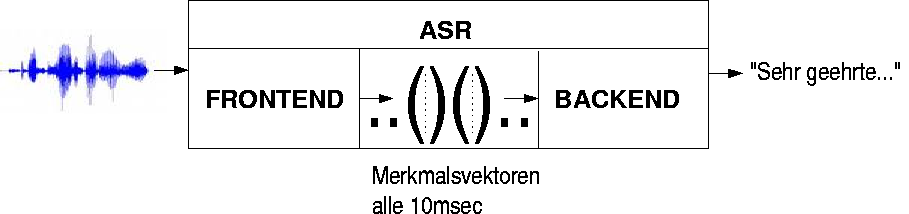
\includegraphics[width=\textwidth]{grafiken/automatische-spracherkennung/struktur.png}

{\bf Frontend}
{\em Der Frontend verarbeitet das Sprachsignal bis hin zu einer 
Reihe von Merkmalsvektoren, welche in regelmäßigem zeitlichem 
Abstand angeordnet sind (z.\,B. alle 10msec). Ein Merkmalsvektor
enthält als Elemente quantifizierbare phonetische Merkmale des 
Teilstücks im Sprachsignal um die Position des Merkmalsvektors
(Fenster).}

{\bf Backend}
{\em Der Backend hat 2 Aufgaben zu lösen:}
\vsph
\begi
\item Hypothetische Muster in der Zeitreihe der Merkmalsvektoren 
identifizieren und bewerten (Muster können sich überlappen)
\item Die zeitlich bündige Kombination von Mustern finden, welche die
beste Gesamtbewertung erzielt (z.\,B. einen Satz aus mehreren Wörtern)
\ndit
\vsph
Zur Bewertung von hypothetischen Mustern gibt es viele verschiedene 
Verfahren. Die wichtigsten sind: 
\begi
\item {\em Dynamic Time Warping (DTW, auch manchmal
Dynamic Programming, DP genannt) 
\item Hidden Markov Modelle (HMM) oder 
\item Künstliche Neuronale Netze (ANN)}
\ndit


\section{ASR Strategien}
Zwei grundlegende Strategien: Bottom-up und Top-down

{\bf Bottom-up}

{\em Die Bottom-up Strategie erkennt zunächst eine Kette von möglichst
kleinen linguistischen Einheiten (z.\,B. Laute) und versucht darauf aufbauend,
immer größere Einheiten bis hin zur kompletten Äußerung zu erschließen.}

Beispiel: {\em Halbsilben $\Rightarrow$ Silben $\Rightarrow$ Morphe $\Rightarrow$ Wörter $\Rightarrow$ Satz}

Vorteile / Nachteile:
\begi
\item {+ weniger Kombinatorik (= weniger Suchaufwand = schneller)}
\item {+ bessere Kontrolle über verschiedene linguistische Ebenen}
\item {- Segmentierungsfehler auf unterster Ebene nicht reparierbar}
\item {- Bewertungsfehler auf unterster Ebene schwer reparierbar}
\item {- Phonotaktik und Syntaktik schwer zu integrieren}
\ndit

\centerline{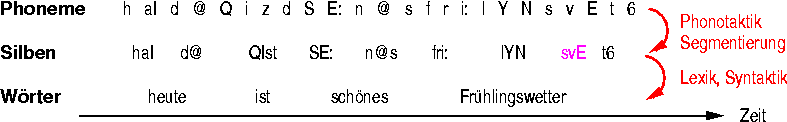
\includegraphics[width=13cm]{grafiken/automatische-spracherkennung/bott.png}}

{\bf Top-Down}

{\em Die Top-Down Strategie konstruiert zunächst eine sehr große Menge
von Kombinationen, schränkt diese durch Ausnutzung der Phonotaktik, Lexik 
und Syntaktik ein und sucht dann innerhalb dieser Kombinationen diejenige,
deren akustische Ähnlichkeit am größten ist.}

Vorteile / Nachteile:
\begi
\item {+ keine Fehlerfortpflanzung möglich (da alle Ebenen gleichzeitig bearbeitet werden)}
\item {+ Phonotaktik, Lexik und Syntaktik einfach integrierbar}
\item {+ Sehr gut vereinbar mit statistischen Verfahren}
\item {+ Fast immer bessere Performanz als Bottom-up Strategie}
\item {- astronomische Anzahl von Kombinationen; sehr intelligente Such-Algorithmen notwendig (Mehrdim. DTW, Viterbi-Decoding)}
\ndit

\centerline{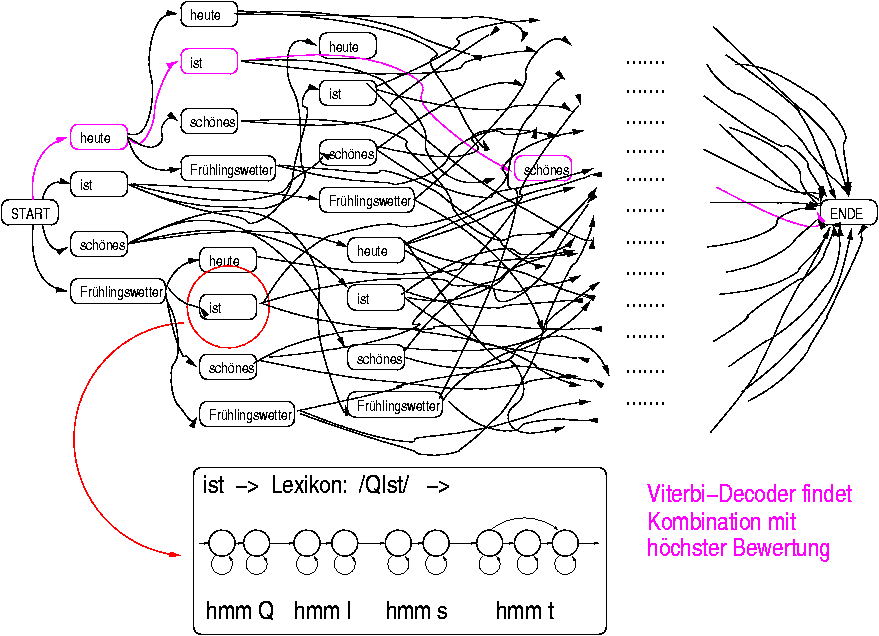
\includegraphics[width=10cm]{grafiken/automatische-spracherkennung/top.png}}

\section{Performanz (Stand 2018)}
Messung in {\em Wort Accuracy} $W_A$ (Wortakuratheit := wieviele gesprochene Wörter erkannt werden) 
auf manuell annotierten Korpora.
\begi
\item Diktieren, Nahbesprechungsmikrophon, sprecheradaptiv, Lexikon 30000-80000, 
eingeschränkte {\em domain}, fließende Sprache: {\em ca. 95 - 98\% $W_A$}
\item Steuerung von Geräten, Nahbesprechungsmikrophon, sprecherunabhängig, Lexikon 10 - 50, 
sehr eingeschränkte {\em domain}, Einzelwörter: {\em ca. 95 - 99\% $W_A$}
\item Dialogsystem, Telephonkanal, sprecherunabhängig, Lexikon 10 - 20, 
sehr eingeschränkte {\em domain}, Einzelwörter: {\em ca. 90 - 99\% $W_A$}
\item Dialogsystem, Nahbesprechungsmikrophon, sprecherunabhängig, Lexikon 1000 - 5000, 
eingeschränkte {\em domain}, Einzelsätze: {\em ca. 95 - 98\% $W_A$}
\ndit

\section{Wichtigste Probleme}
\begi
\item Empfindlichkeit gegen Störgeräusche, {\em cross talk}, Kanalcharakteristik, Reflexionen
\item Fehlerrate steigt mit Lexikongröße
\item Fehlerrate steigt mit sinkender Testsatzperplexität der Syntaktik
\item Gute Performanz fast nur mit Nahbesprechungsmikrophonen ({\em headset})
\item Großer Wortschatz erfordert Sprecheradaption (einige Stunden Training) und 
Einschränkung der {\em domain} (z.\,B. Geschäftsbriefe, Röntgendiagnostik)
\item ASR hat kein 'Weltwissen', ambiger Input ist schwer auflösbar
\item Evaluierungsergebnisse sind stochastischer Natur und schwer vergleichbar,
daher {\em benchmarks} (Wettbewerbe) unter gleichen Bedingungen
\item Realistische Sprachdatenkorpora sind schwer zu produzieren, zuviele Faktoren:
Alter, Geschlecht, Dialekt, soziale Herkunft, Gesundheits-/Gemütszustand
\ndit

\section{Zusammenfassung}
\begi
\item ASR ist nicht programmierbar wegen hoher Variabilität der Sprache
\item Lösung: Maschinelles Lernen auf großen Sprach-Korpora
\item Struktur: Frontend (Sprachsignal -$>$ Merkmale), Backend (Mustererkennung, Suche)
\item Merkmale: meistens spektral basiert, Cepstren, gehörgerechte Skalen
\item 2 Suchstrategien: {\em Bottom-up und Top-down}
\ndit

\section{Literatur}

        {\em Gute Einführung:}\\
%        Euler S (2006): Grundkurs Spracherkennung. Vieweg Wiesbaden.\\
        Pfister, B. \& Kaufmann, T. (2008). Sprachverarbeitung - Grundlagen und 
	Methoden der Sprachsynthese und Spracherkennung. 
	Springer-Verlag Berlin Heidelberg.

%        {\em Die Verwendung von ANN in der ASR:}\\
%	Bourlard H, Morgan N (1994): Connectionist Speech Recognition - 
%	A Hybrid 
%	Approach Kluwer Academic Publishers, Engineering and Computer 
%	Science.
%       {\em Beispiel für eine spezielle Merkmalsextraktion:}\\
%	Hermansky H, Morgan N, Bayya A, Kohn P (1991): Compensation for 
%	the Effect of the Communication Channel in Auditory-Like Analysis 
%	of Speech (RASTA-PLP), EUROSPEECH 1991, Genua, p. 1367 - 1370.

 %       {\em Grundlegender Artikel über das Viterbi-Training von HMM:}\\
%	Juang B H, Rabiner L R (1990): The segmental k-means algorithm for 
%	estimating parameters of Hidden Markov Models.
%	IEEE Transactions on Acoustics, Speech and Signal Processing, Vol. 38, 
%	No. 9, Sep 1990, S. 1639 - 1641.	

        {\em Einführung in ANN:}\\
	Lippmann, R. S. (1987). An Introduction to Computing with Neural Nets.
	IEEE. ASSP Magazine. April 1987. S.\,4 - 22.

%        {\em Einführung über Dynamic Time Warping als Mustererkennung:}\\
%	Ney H, Ortmanns S (1999): Dynamic Programming Search for 
%	Continuous Speech Recognition. in: IEEE Signal Processing Magazine, 
%	Sept 1999, pp. 64-83.

 %       {\em Gute Einführung in HMM in der ASR:}\\
%	Picone J (1990): Continuous Speech Recognition Using Hidden Markov Models.
%	IEEE ASSP Magazine, Jul 1990, S. 26 - 41.

 %       {\em Grundlegender Artikel über HMM:}\\
%	Rabiner L R, Juang B H (1996): An Introduktion to Hidden Markow Modells
%	IEEE ASSP Magazine, Jan 1986, p. 4.

%	{\em Einführendes Buch über Akustische Phonetik; Kapitel 2.4 - 2.8 sind 
%	sehr gute Erklärungen zum digitalen Signal und Spektrum:}\\
%	Reetz H (2003): Artikulatorische und akustische Phonetik, 
%	Wissenschaftlicher Verlag Trier.

        {\em Gutes Lehrbuch über alle Arten von Sprachverarbeitung:}\\
        Jurafsky D. \& Martin J. H. (2000). Speech and Language Processing. 
	Prentice Hall. Kap I.7.

%        {\em Mathematische Theorie der Spracherkennung; ziemlich schwierig; 
%	interessant (auch ohne viel Mathe-Kenntnisse): Kapitel 7:}\\
%        Levinson S (2005): Mathematical Models for Speech Technology, John Wiley \& Sons, UK.

%        {\em Wissenschaftliches Arbeiten:}\\
%        Bördlein S (2002): Das Sockenfressende Monster in der Waschmaschine. Alibri Verlag Gunnar Schedel.







%\maketitle


%\begin{figure}[htbp]
%\begin{center}
%\includegraphics[width=\textwidth]{diagramme/topographie_sdb}
%\label{fig_topo_sdb}
%\end{center}
%\end{figure}

\chapter{Sprachsynthese}

%\maketitle

  %%%%%%%%%%%%%%%%%%%%%%%%%%%%%%%
  %%%%%%%%%%%%%%%%%%%%%%%%%%%%%%%
  \section{Übersicht}
  
  Kurze Definition: \emph{Unter Sprachsynthese versteht man die künstliche Erzeugung der menschlichen Sprechstimme.}

\begin{figure}[htbp]
\begin{center}
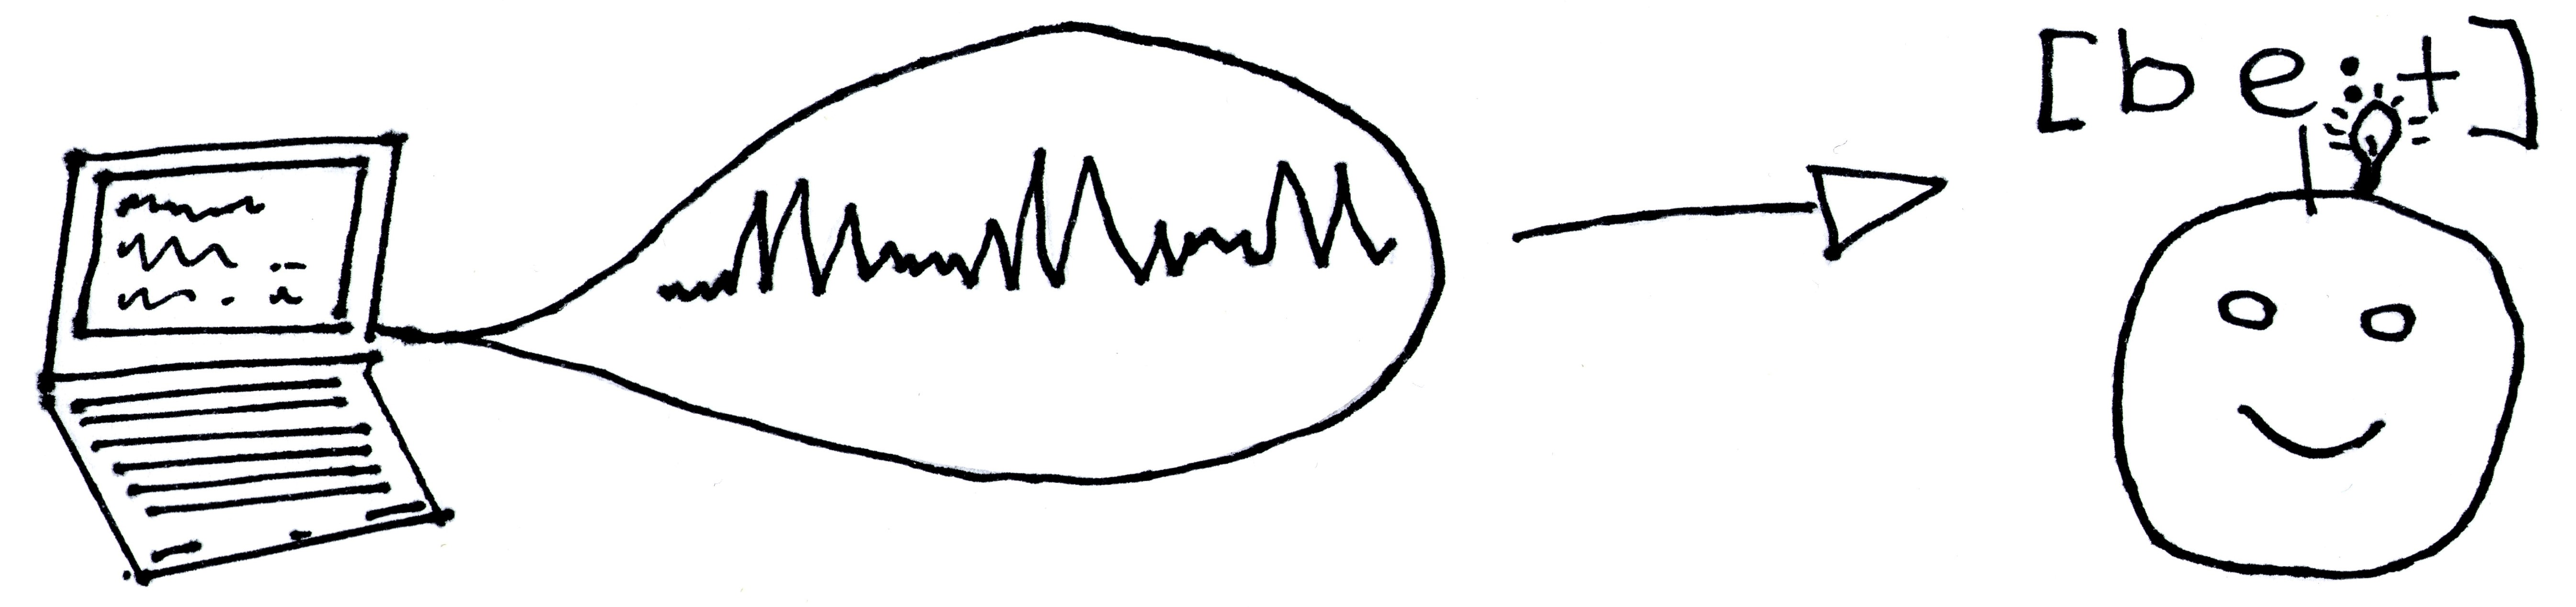
\includegraphics[width=\textwidth]{grafiken/sprachsynthese/synthese}
\label{ts}
\end{center}
\end{figure}
  %%%%%%%%%%%%%%%%%%%%%%%%%%%%%%%
  %%%%%%%%%%%%%%%%%%%%%%%%%%%%%%%
  \section{Typologie von Synthesesystemen}

  %%%%%%%%%%%%%%%%%%%%%%%%%%%%%%
  \textbf{Reichweite}

  \begin{itemize}
  \item Concept-to-Speech CTS:
  \emph{Semantisches Konzept $\longrightarrow$ Text $\longrightarrow$ akustisches Signal}
  \item  Text-to-Speech TTS: \emph{Text $\longrightarrow$ akustisches Signal}
  \end{itemize}\newpage

  %%%%%%%%%%%%%%%%%%%%%%%%%%%%%%
  \textbf{Art der Synthese}

  \begin{itemize}
  \item Formantsynthese: \emph{Generierung und Hörbarmachung künstlicher Sonagramme}
  \item Artikulatorische Synthese: \emph{Artikulationsmodell $\longrightarrow$ Akustik}
  \item Konkatenative Synthese:  \emph{Verkettung von phonetischen Segmenten aus einer Datenbank}
  \end{itemize}
  
  %%%%%%%%%%%%%%%%%%%%%%%%%%%%%%
  %%%%%%%%%%%%%%%%%%%%%%%%%%%%%%
  \section{Architektur}

  \begin{figure}[!htbp]
  \begin{small}
  \centerline{
  \xymatrix@! C=3cm {
  Text \ar[4,0] & Textnormalisierung \ar[1,0] & (Computer-)linguistik \ar[2,0]\\
  & Linguistische \textrm{ } Analysen  \ar[1,0] & \\
  & Graphem-Phonem-Konvertierung  \ar[1,0] & Phonetik \ar[2,0]\\
  & Prosodie-Generierung  \ar[1,0] & \\
  Signal & Akustische \textrm{ } Gen. & Phonetik, E-Technik
  }
  }
  \end{small}
  \end{figure}

  %%%%%%%%%%%%%%%%%%%%%%%%%%%%%%%
  %%%%%%%%%%%%%%%%%%%%%%%%%%%%%%%
  \section{Textnormalisierung}
  
  \begin{itemize}
  \item \emph{Satzsegmentierung} (Disambiguierung der Interpunktion)
  \item \emph{Expansion} von Titeln, Abkürzungen, Ziffernfolgen etc.
  \item Beispiel: 
  \begin{itemize}
  \item am 2. $\longrightarrow$ zweit\emph{en}
  \item der 2. $\longrightarrow$ zweit\emph{e}
  \item 1980 Studenten $\longrightarrow$ eintausendneunhundertachtzig
  \item im Jahr 1980 $\longrightarrow$ neunzehnhundertachtzig
  \item die Durchwahl lautet 1980 $\longrightarrow$ eins neun acht null
  \end{itemize}
  \item mittels lokaler Grammatiken: 1980 $\longrightarrow$ neunzehnhundertachtzig $|$ Jahr \_\_
  \end{itemize}

  %%%%%%%%%%%%%%%%%%%%%%%%%%%%%%
  %%%%%%%%%%%%%%%%%%%%%%%%%%%%%%
  \section{Linguistische Analysen}

  \begin{itemize}
  \item Zuweisung der \emph{Wortarten} (Part-of-Speech-Tagging)
  \item ggf. \emph{syntaktische} Analyse
  \item ggf. \emph{semantische} Analyse, Fokuslokalisierung
  \item Fokus:
  \begin{itemize}
  \item \emph{Informationszentrum} einer Äußerung
  \item neue Information oder Kontrast
  \end{itemize}
  \item relevant für die Prosodie der Äußerung
  \end{itemize}

  %%%%%%%%%%%%%%%%%%%%%%%%%%%%%%%
  %%%%%%%%%%%%%%%%%%%%%%%%%%%%%%%
  \section{Graphem-Phonem-Konvertierung}

  \begin{itemize}
  \item Überführung der Buchstabenfolge in eine Transkription
  \end{itemize}

  %%%%%%%%%%%%%%%%%%%%%%%%%%%%%%%%
  \subsection*{Table Lookup-Verfahren (van den Bosch et al., 1993)}

  \begin{itemize}
  \item sprachunabhängiger rein datenbasierter Ansatz
  \item \emph{Training: Erstellung einer Graphem-Phonem-Tabelle}

  \begin{tabular}{|l|l|}
  \hline
  linker Kontext+\emph{Zielgraphem}+rechter Kontext & \emph{Zielphonem}\\
  \hline
  b+\emph{u}+n & \emph{/U/} \\
  q+\emph{u}+a & \emph{/v/} \\
  \hline
  \end{tabular}

  \item Anwendung: Nachschlagen in der Tabelle
  \begin{itemize}
  \item ``Q\emph{u}alle'':  q+u+a $\longrightarrow$ \emph{/v/}
  \item ``B\emph{u}nd'': b+u+n $\longrightarrow$ \emph{/U/}
  \end{itemize}
  \end{itemize}

  %%%%%%%%%%%%%%%%%%%%%%%%%%%%%%%
  \section{Prosodische Modellierung}

  \begin{itemize}
  \item Ermittlung der \emph{prosodischen Struktur}
  \item Modellierung von \emph{Grundfrequenzverlauf} und \emph{Lautsegmentdauern}
  \end{itemize}

  %%%%%%%%%%%%%%%%%%%%%%%%%%%%%%%
  \subsection*{Prosodische Struktur}

  \begin{itemize}
  \item Phrasengrenzen: Gliederung einer Äußerung
  \item Akzente: Hervorhebung wichtiger Äußerungsteile
  \item Beispiel: 
  \begin{itemize}
  \item Der \emph{Bundestag} $|$ setzte seine \emph{Debatte} $|$ heute \emph{fort}. $|$ (Grenzen $|$, Akzentuierte Wörter \emph{kursiv})
  \end{itemize}
  \end{itemize}

  %%%%%%%%%%%%%%%%%%%%%%%%%%%%%%%
  \subsection*{Lokalisierung von Phrasengrenzen}
  
  \begin{itemize}
  \item \emph{Chink-Chunk-Algorithmus} (Liberman et al., 1992):
  \begin{itemize}
  	\item \emph{Chink-Wortarten} (Präpositionen, Artikel, \ldots) \emph{phraseninitial}
  	\item \emph{Chunk-Wortarten} (Substantive, Verbpatikel, \ldots) \emph{phrasenfinal}
  \end{itemize}
  \item Chunk-Wörter im obigen Beispiel: \emph{Bundestag, Debatte, fort}
  \end{itemize}

  \begin{itemize}
  \item Je \emph{unvorhersagbarer} ein Wort, desto eher ist es akzentuiert
  \item Beispiel: \emph{Kritik} zu üben \emph{vs.} Kritik zu \emph{ignorieren}
  \item Ermittlung der Vorhersagbarkeit eines Worts $w$:
  \begin{itemize}
  \item kontextunabhängige \emph{Auftretenswahrscheinlichkeit} $P(w)$ 
  \item kontextabhängige \emph{bedingte Wahrscheinlichkeit} $P(w|\textrm{Wortumgebung})$
  \end{itemize}
  \end{itemize}

  %%%%%%%%%%%%%%%%%%%%%%%%%%%%%%%%%%%%%%%%%%
  \subsection*{Modellierung des Grundfrequenzverlaufs}

  \begin{itemize}
  \item \emph{Fujisaki-Modell} (Fujisaki, 1987):
  \begin{itemize}
  \item \emph{superpositional:} Addition von globaler Phrasenkontur und lokalen Akzentkonturen
  \item Initiierung durch \emph{Phrasenkommandos} zu Beginn prosodischer Phrasen und \emph{Akzentkommandos} auf akzentuierten Silben.
  \end{itemize}
  \end{itemize}
  
  \begin{figure}[htbp]
\begin{center}
  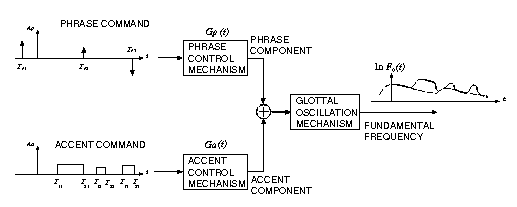
\includegraphics[width=\textwidth]{grafiken/sprachsynthese/fujisaki-pic.png}
  \caption{Fujisaki-Modell}
  \end{center}
  \end{figure}

  %\includegraphic{Missing fujisaki pic}


  %%%%%%%%%%%%%%%%%%%%%%%%%%%%%%%%%%%%%%%%%%%%%%
  \subsection*{Modellierung der Lautdauern}
  
  \begin{itemize}
  \item $\hat{d}(x) = f \cdot \bar{d}(x)$
  \item \emph{intrinsische Lautdauer} $\bar{d}(x)$ des Lauts $x$
  \begin{itemize}
  \item z.\,B. mittlere Dauer von $x$ in einem segmentierten Korpus
  \item für Vokale höher als für Konsonanten
  \item für tiefe Vokale höher als für hohe Vokale
  \end{itemize}
  \item \emph{Anpassungsfaktor} $f$
  \begin{itemize}
  \item zur Umwandlung der intrinsischen Dauer in die \emph{realisierte Dauer} $\hat{d}(x)$ des Lauts $x$
  \item abhängig von Einflussfaktoren, wie:
  \item \emph{Prosodie:} Silbe akzentuiert $\longrightarrow$ Erhöhung der Dauer, d.\,h. $f>1$
  \item \emph{Lautkontext:} stimmloser Obstruent folgt $\longrightarrow$ Verringerung der Dauer von Vokalen, d.\,h. $f<1$
  \end{itemize}
  \end{itemize}

\newpage


  %%%%%%%%%%%%%%%%%%%%%%%%%%%%%%
  \section{Akustische Generierung}
  
  %%%%%%%%%%%%%%%%%%%%%%%%%%%
  \subsection*{Input}

  \begin{itemize}
  \item Transkription (von Graphem-Phonem-Konvertierung)
  \item für jedes Phon:
  \begin{itemize}
  \item Grundfrequenz-Werte (von prosodischer Modellierung)
  \item Dauerangabe (von prosodischer Modellierung)
  \end{itemize}
  \end{itemize}

  %%%%%%%%%%%%%%%%%%%%%%%%
  \subsection*{Beispiel: Konkatenative Synthese (\emph{Unit selection})}

  \begin{itemize}
  \item Verkettung von phonetischen Einheiten, z.\,B. \emph{Diphonen}
  \item \emph{Diphon:} Segment von Mitte eines Phons bis zur Mitte des folgenden Phons
  \item dadurch Berücksichtigung der \emph{koartikulatorisch bedingten akustischen Variation} $\longrightarrow$ wichtig für Natürlichkeit und Verständlichkeit der Synthese
  \end{itemize}

 
 \begin{figure}
 \begin{center}
 \begin{minipage}[ct]{0.2\textwidth}
 
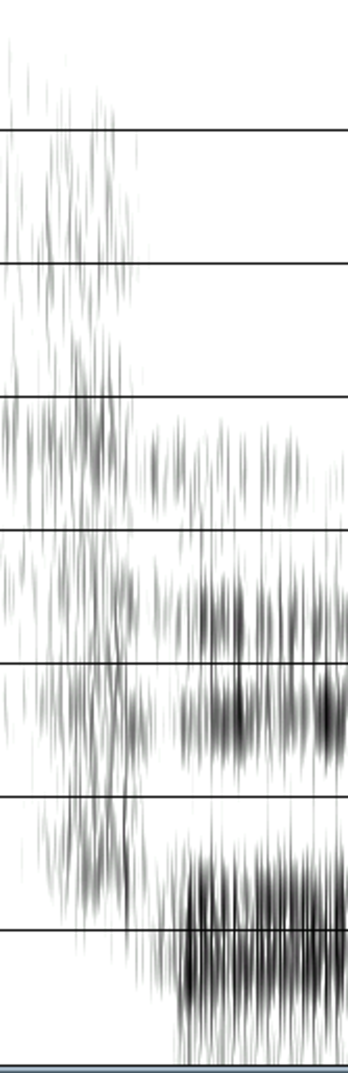
\includegraphics[width=1\textwidth]{grafiken/sprachsynthese/fa}
\end{minipage}
\hspace{2cm}
\begin{minipage}[ct]{0.2\textwidth}
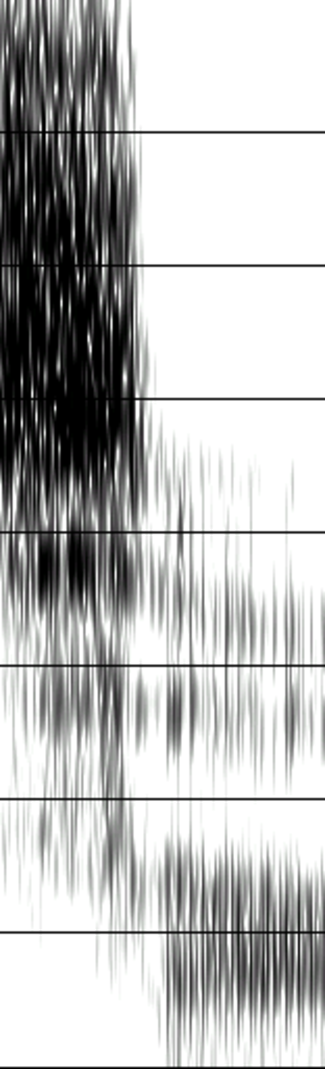
\includegraphics[width=1\textwidth]{grafiken/sprachsynthese/sa}
\end{minipage}
\end{center}
\caption {Diphone /fa/ und /sa/: unterschiedliche F2-Transitionen.}
\end{figure}
 
 


\begin{itemize}
\item {\bf Inventar:}
\begin{itemize}
\item $40^2=1600$ \emph{potentielle Phonemkombinationen}, eingeschränkt durch \emph{Phonotaktik}
\item jedes Diphon-Type in \emph{mehrfacher Realisierung} in der Datenbank gespeichert
\item \emph{Types:} unterschiedliche Diphone, /fa/ vs. /sa/;\\\emph{Realisierung:} /fa/$_1$, /fa/$_2$ etc.
\end{itemize}
\item \emph{Verkettung:}
\begin{itemize}
\item \emph{Transkription} $\longrightarrow$ Wahl der Diphon-Types
\item \emph{Lautliche Umgebung, Prosodie} $\longrightarrow$ Wahl der am besten passenden gespeicherten Diphon-Realisierung 
\end{itemize}
\end{itemize}

\begin{itemize}
\item \emph{Auswahl der bestgeeigneten Diphon-Realisierung}
\begin{itemize}
\item anhand einer \emph{Kostenfunktion}
\item \emph{Target-Kosten:} wie stark weicht Diphon von geforderter Grundfrequenz, Dauer etc. ab?
\item \emph{Join-Kosten:} wie gut passt Diphon zum vorangehenden Diphon?
\end{itemize}
\end{itemize}

%%%%%%%%%%%%%%%%%%%%%%%%%%%%%%
\subsection*{Synthesebeispiele}

\url{http://ttssamples.syntheticspeech.de/deutsch/}


%%%%%%%%%%%%%%%%%%%%%%%%%%%%%%
%%%%%%%%%%%%%%%%%%%%%%%%%%%%%%
\section{Literatur}


\emph{Eine gute Einführung findet sich in Kapitel 8:}\\
Jurafsky, Dan \& Martin, James H. (2000): Speech \& language processing. Pearson Education India

\emph{Kapitel 3 in:}\\
Pfister B., Kaufmann T. (2008): Sprachverarbeitung - Grundlagen und 
	Methoden der Sprachsynthese und Spracherkennung. 
	Springer-Verlag Berlin Heidelberg.


\renewcommand\refname{\vskip -1cm}
\bibliography{synthese}{}
\bibliographystyle{plain}

%%%%%%%%%%%%%%%%%%%%%%%%%%%%%%
%%%%%%%%%%%%%%%%%%%%%%%%%%%%%%








\chapter{Psycholinguistik}
\begin{figure}[htbp]
\begin{center}
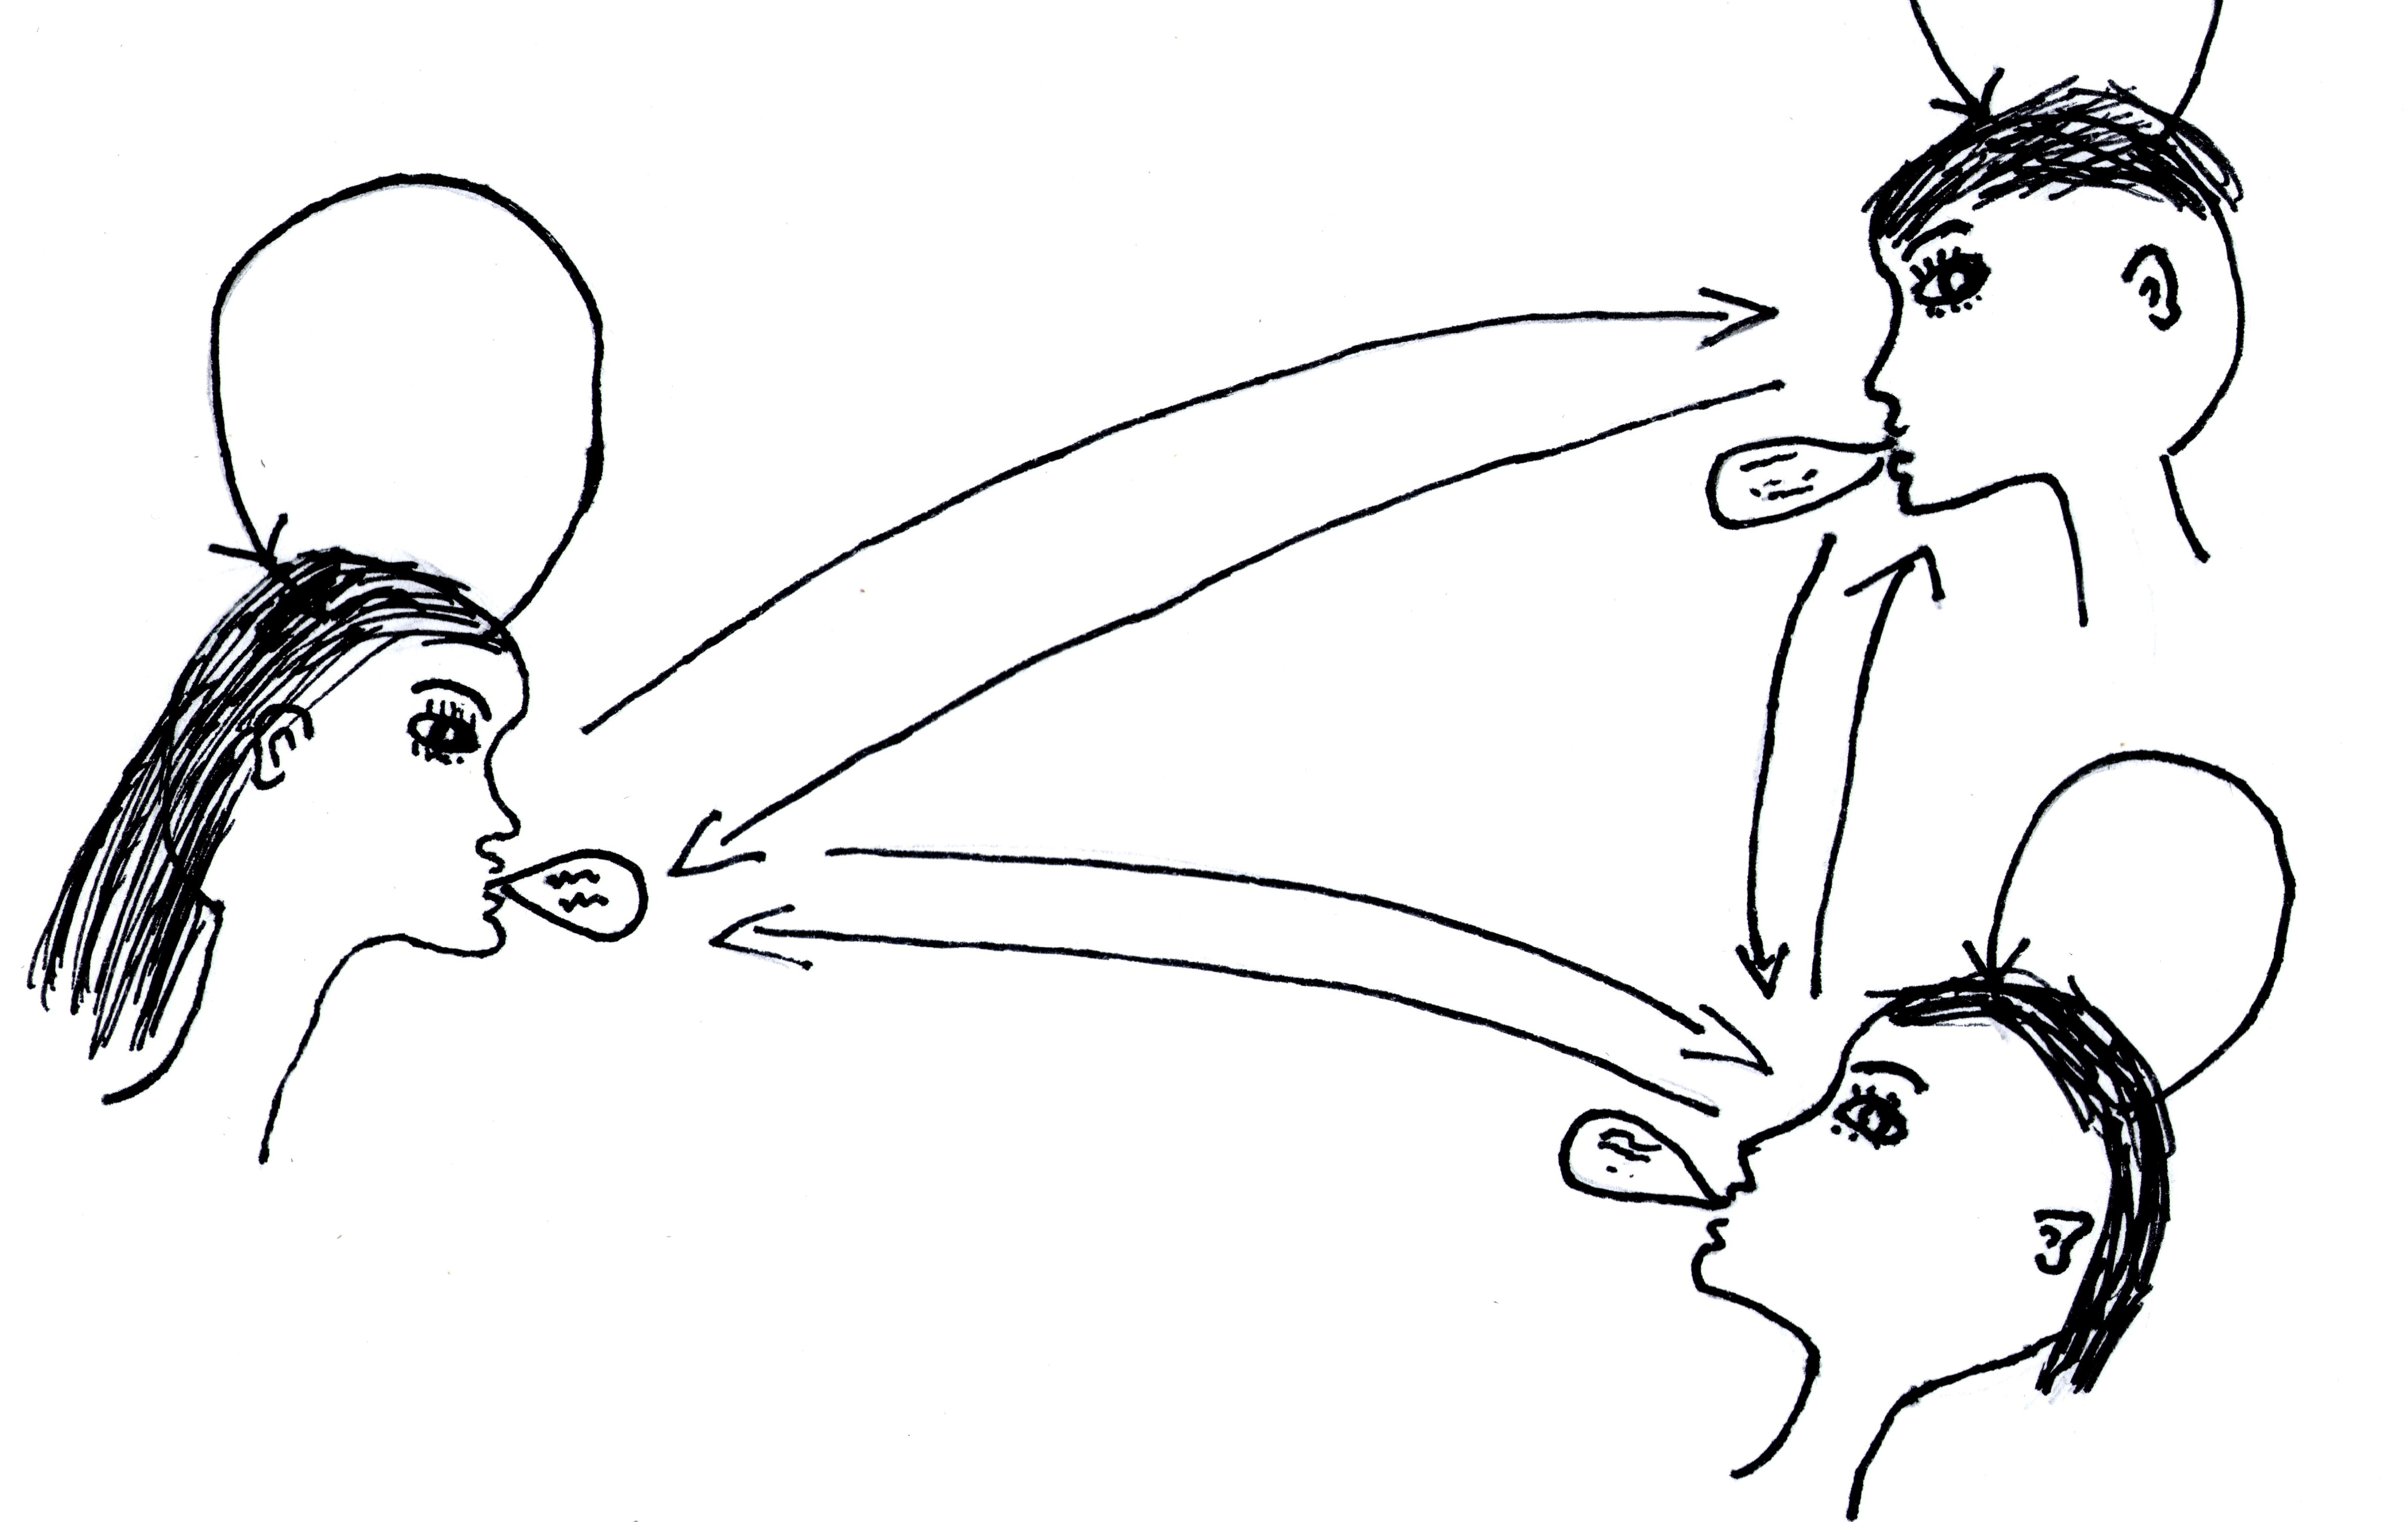
\includegraphics[width=0.6\textwidth]{grafiken/psycholinguistik/psycholinguistik}
\label{t9}
\end{center}
\end{figure}
\section{Übersicht}
Die Psycholinguistik interessiert sich für die sprachliche Tätigkeit des Menschen. Es handelt sich bei der Psycholinguistik um eine Forschungsdisziplin, die 1953/54 in den USA als interdisziplinäre Disziplin von Psychologen, Linguisten, Informations- und Kommunikationswissenschaftlern, Medizinern und Anthropologen gegründet wurde (Osgood \& Sebeok, 1954). Grundidee war, die Polarität von Linguistik und Psychologie zu überwinden. Zentrale Forschungsbereiche, die nach dieser Gründung entstanden sind, können folgendermaßen benannt werden (vgl. Cutler, Klein \& Levinson 2005; Dietrich 2007):

\textbf{Fachbereiche}

1)	Sprachwissen (Mentales Lexikon, Grammatisches Wissen)\\
2)	Spracherwerb (Erstspracherwerb, Bilingualismus, Zweitspracherwerb)\\
3)	Sprachverarbeitung (Sprachverstehen, Sprachproduktion)\\
4)	Sprache und Kognition (Genese von Sprache und Kognition, Zusammenhang von Sprache und Kognition)\\
5)	 Schriftlichkeit und Mündlichkeit (Konzipierung von Schriftlichkeit und Mündlichkeit, Funktionaler Analphabetismus)\\
6)	Rhetorik (Klassische Rhetorik, Angewandte Rhetorik)\\
7)	Sprachpathologie (Sprachentwicklungsstörungen, Erworbene Sprach- und Sprechstörungen)\\

Im signalphonetischen Band lässt sich eine Verbindung zwischen den neuronalen und psychischen Prozessen des Sprechers und des Hörers herstellen. Es handelt sich hier um die „Pole“ eine Kommunikation. In der Wechselwirkung der Schallphänomene entstehen dialogische Strukturen, d.\,h. Sprechen umfasst vor allem immer auch soziale Prozesse. Diese dazwischenliegenden Strukturen sind aufgrund der jeweiligen Spezifik (Intention, Adressierung, Positionierung, Kontext) nur schwer korrelierbar.


\section{Experimentelle Psycholinguistik}
Stichpunkte: Mentales Lexikon, Grammatisches Wissen, Sprachverarbeitung\\
\\
Die experimentelle Psycholinguistik beschäftigt sich mit den Prozessen, die bei der Verarbeitung gesprochener Sprache stattfinden. Ihr Ziel ist es, Hypothesen zu theoretischen Modellen der Sprachverarbeitung empirisch zu testen.\\
\begin{figure}[htbp]
\begin{center}
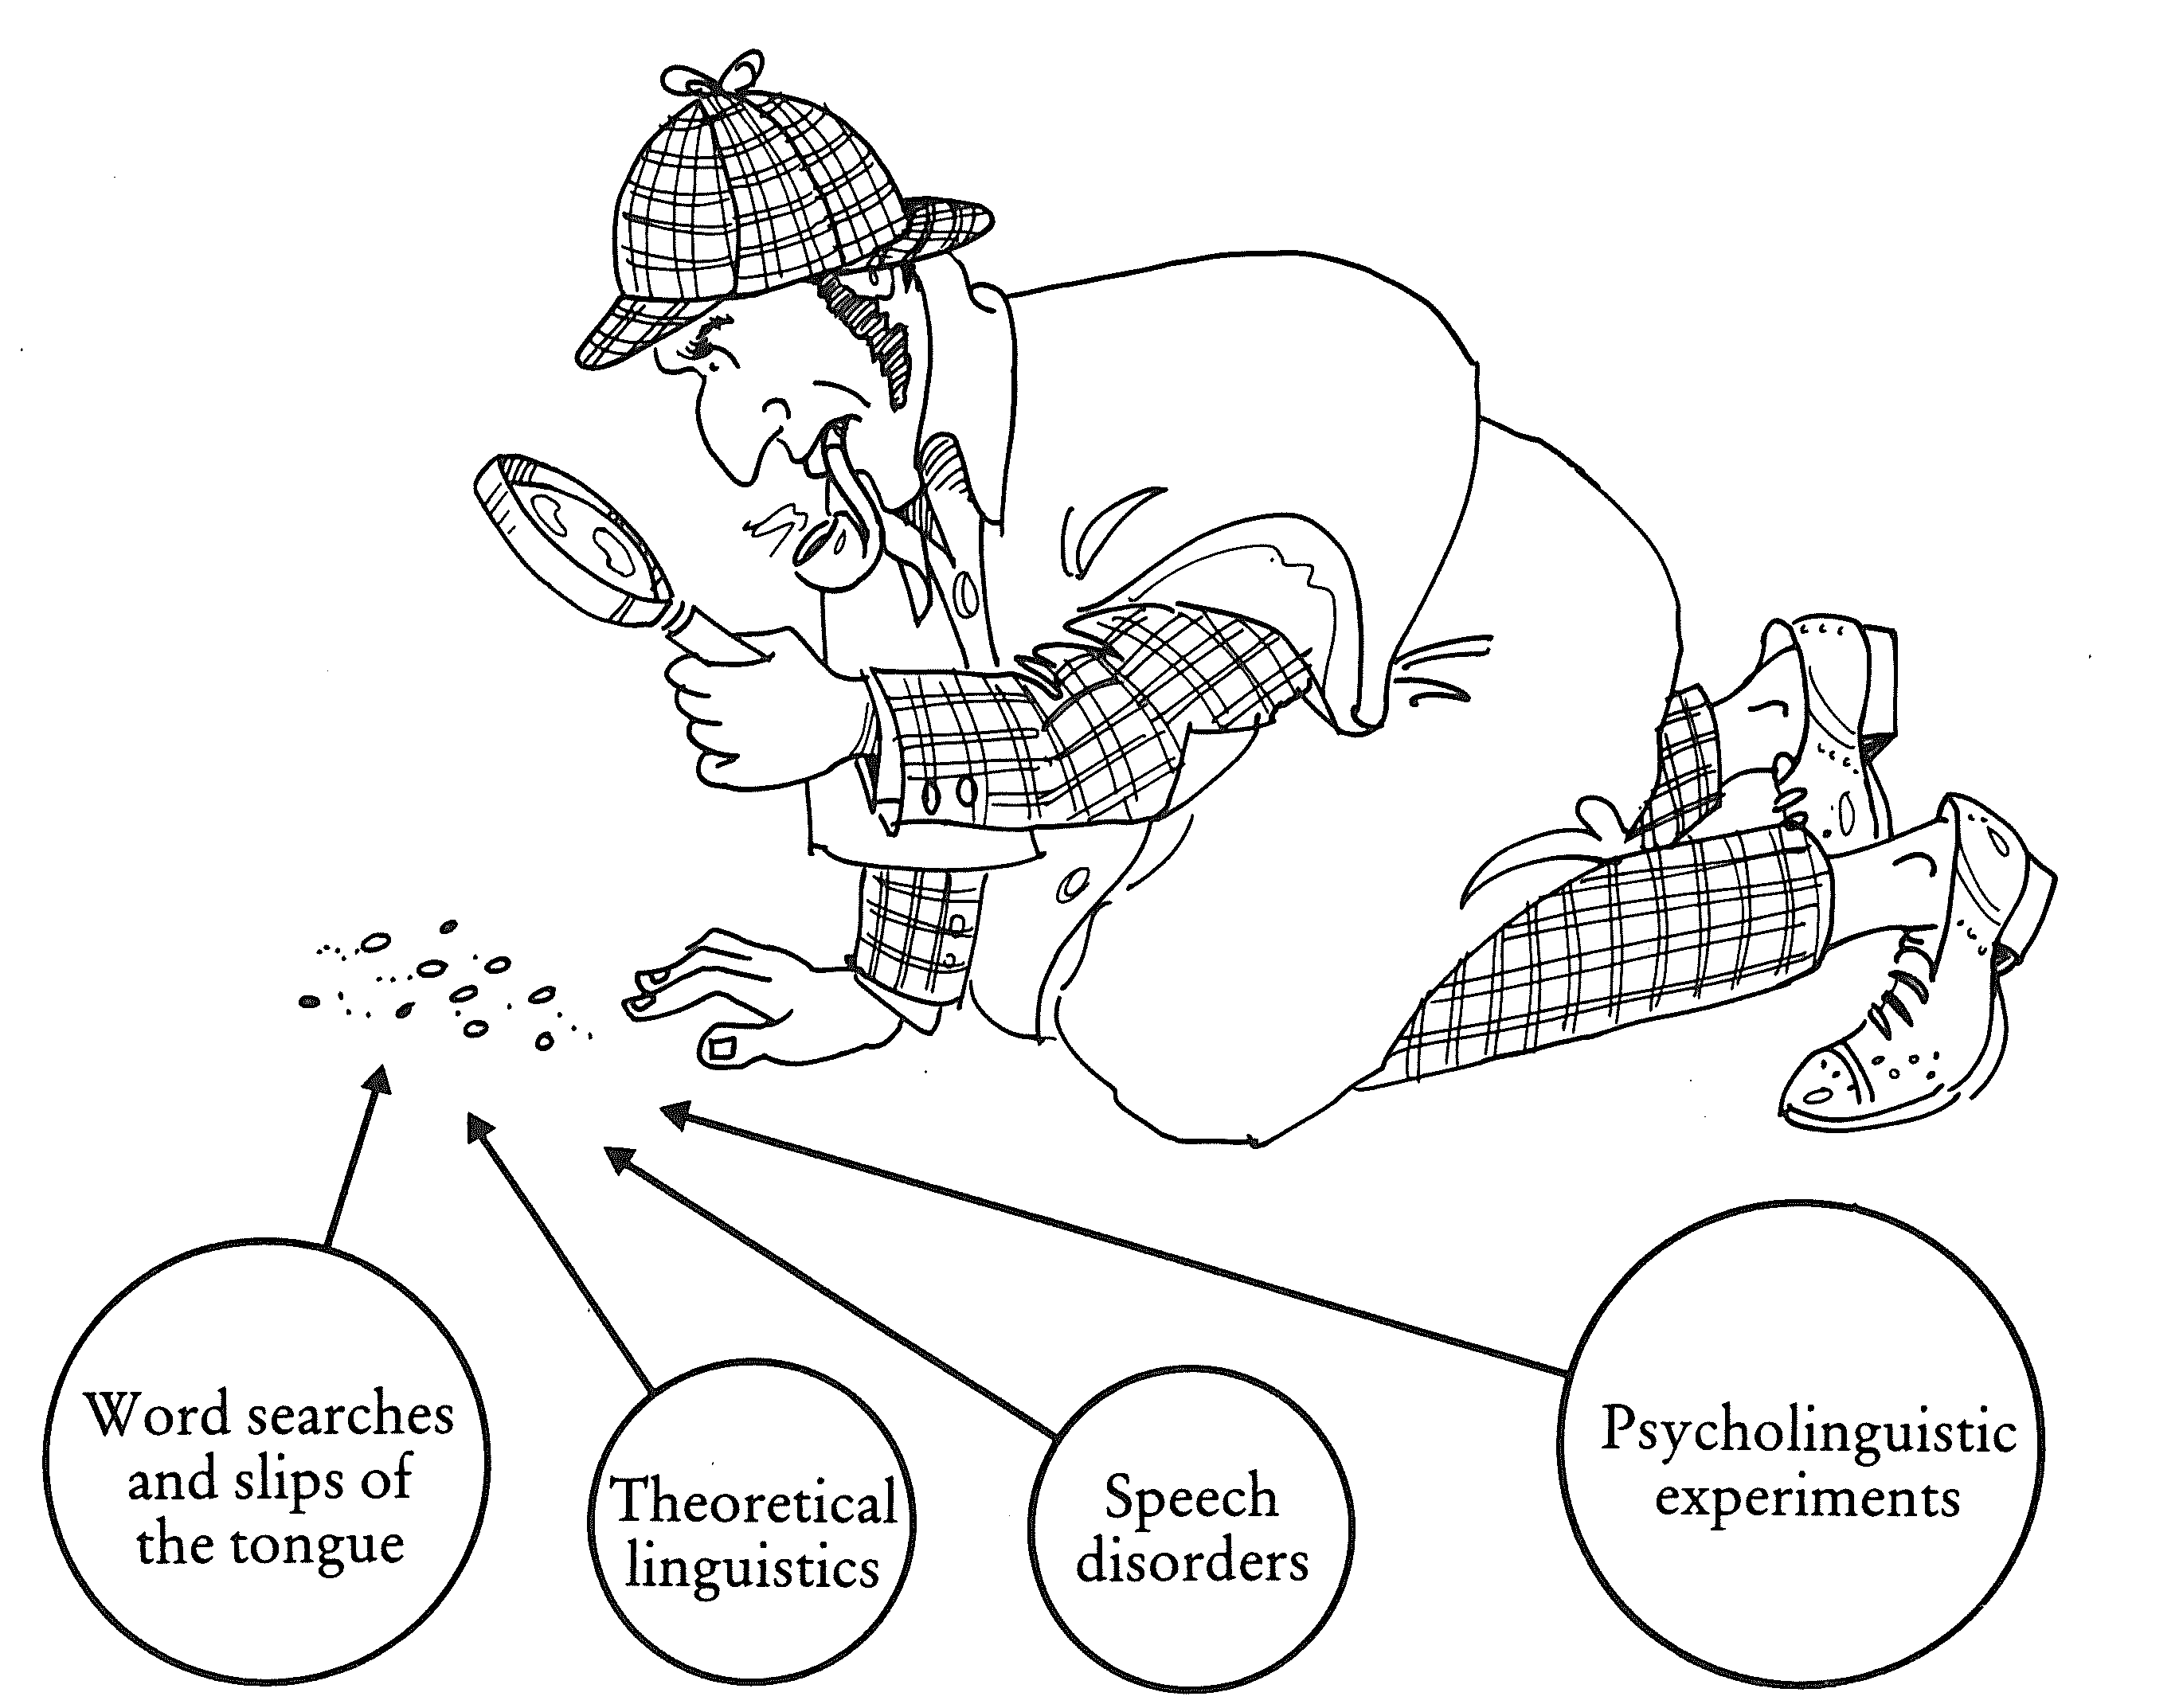
\includegraphics[width=0.5\textwidth]{grafiken/psycholinguistik/detektiv}
\caption{Aitchinson, J. (2012). Words in the Mind: An Introduction to the Mental Lexicon. West Sussex: John Wiley \& Sons. S. 19.}
\label{psy1}
\end{center}
\end{figure}
\newpage


\textbf{Fragestellungen}

Was könnten typische Fragestellungen in der Psycholinguistik sein? Welche Frage würden Sie gern untersuchen?

Diskutieren Sie, welche Ereignisse beobachtet und gemessen werden können. Was bedeutet das für psycholinguistische Experimente und deren Aussagen über mentale Prozesse?

\vspace{1cm}

\textbf{Eyetracking}

Lesen Sie den Textausschnitt zum Eyetracking. Diskutieren Sie, welche Vorteile diese Methode hat und worauf beim Erstellen eines Experiments besonders geachtet werden muss.


\vspace{1cm}

\textbf{Erstspracherwerb – Fremdspracherwerb}

Überlegen Sie in der Gruppe, was die Merkmale des Erst- und des Fremdspracherwerbs sind. Wie unterscheiden sich die beiden voneinander?

Überlegen Sie sich ein Beispiel und formulieren Sie eine wissenschaftliche Frage zum Fremdspracherwerb, die Sie gerne testen würden.





\section{Verknüpfungen im Fach (Lehrinhalte)}
Psycholinguistische Inhalte werden im BA Phonetik und Sprachverarbeitung in folgenden Modulen vertieft:
P2 – Kognitive Sprachverarbeitung 1 (Psycholinguistik 1 und 2, Sprache \& Kognition 1)
P8 – Kognitive Sprachverarbeitung 2 (Psycholinguistik 3, Sprache und Kognition 2)
P9 – Experimentalphonetik III (Neurophysiologie der Sprache)

\section{Literatur-Auswahl}
Aitchinson, J. (2012\super{4}). Words in the Mind: An Introduction to the Mental Lexicon. West Sussex: John Wiley \& Sons. \newline\\
Cutler, A.; Klein, W. \& Levinson, S. C. (2005). \textit{The cornerstones of twenty-first century psycholinguistics}. In: Twenty-first century psycholinguistics. Four cornerstones. Hg. von Anne Cutler.  Mahwah, New Jersey, London: Lawrence Erlbaum. 1–20.\newline\\
Dietrich, R. (2007). Psycholinguistik. Stuttgart, Weimar: J. B. Metzler.\newline\\
Göttert, K. H. (1991). Einführung in die Rhetorik. München: Wilhelm Fink Verlag.\newline\\
Huettig, F., Rommers, J., Meyer, A. S. (2001). Using the visual world paradigm to study language processing: A review and critical evaluation, Acta Psychologica, 137, Issue 2, 151-171\newline\\
Grimm, H. \& Weinert, S. (2002). \textit{Sprachentwicklung}. In: Oerter, R.; Montada, L. (Hrsg.): Entwicklungspsychologie (S. 517-550). Weinheim u.\,a.: Beltz.\newline\\
Herrmann, C.; Fiebach, C. (2004). Gehirn \& Sprache. Frankfurt am Main.\newline\\
Knobloch, Clemens (2003). \textit{Geschichte der Psycholinguistik}. In: Gerd R.; Herrmann, T. und Deutsch, W. (Hrsg.): Psycholinguistik. Psycholinguistics. Ein internationales Handbuch. An international handbook. Berlin, New York: Walter de Gruyter. 15–33.\newline\\
Koch, P. \& Oesterreicher, W. (1994). \textit{Schriftlichkeit und Sprache}. In: Günther, H.; Ludwig, O. (Hrsg.): Schrift und Schriftlichkeit. HSK. Berlin, New York: de Gruyter.\newline\\
Levelt, W. J. M.(1989). Speaking. From Intention to Articulation. Cambridge, MA; London: MIT Press.\newline\\
Osgood, C. E., und Thomas A. S. (Hrsg) (1954). \textit{Psycholinguistics. A survey of theory and research problems. Report of the 1953 summer seminar sponsored by the Committee on Linguistics and Psychology of the Social Science Research Council}. Baltimore: Waverly Press.\newline\\
Vygotskij, L. S. (1934/2002). Denken und Sprechen. Weinheim und Basel: Beltz.\newline\\






\end{document}
